\documentclass[conference, a4paper]{IEEEtran}
%
\usepackage[T1]{fontenc} % optional
\usepackage{times}
\usepackage[cmex10]{amsmath}
\usepackage{calc}
\usepackage{amsfonts} % to load math symbols
\usepackage{mdwmath}
\usepackage{commath}
\usepackage{mdwmath}
\hyphenation{op-tical net-works semi-conduc-tor}

\usepackage[noadjust]{cite}
\usepackage[keeplastbox]{flushend}
\usepackage{graphicx}
\usepackage{color}
\usepackage{placeins}
\usepackage{float}
\usepackage{booktabs}
\usepackage{standalone}
\usepackage{filecontents}
\usepackage{subfig}
\usepackage{tabularx,colortbl}
\usepackage{pgfplots}
\usepackage{standalone}
\usepackage{tikz}
\tikzset{
font={\fontsize{10pt}{10}\selectfont}}
\usepackage{tikzscale} % Scale the figure not the font
\pgfplotsset{compat=newest}
%% the following commands are sometimes needed
\usepackage{grffile}
\usepackage{mathtools,amssymb}
\usepackage{siunitx}
\sisetup{per=slash, load=abbr}
% \usepackage[a4paper, left=.63in,right=.63in,top=.75in,bottom=1in]{geometry}

%%%%%%%%%%
%%%%%%%%%% TIPS and TRICKS
%%%%%%%%%%
%
% ------------------------------- Useful Tricks Learnt
% Use ={}& to align subequations to the left
% Use = for single equations
% Use &= for split equations
% Use commath package to properly write differential operators and derivatives.
% Use \int\limits to nicely put integral limits
% For long equations, use align environment with \notag\\ as a linebreak.
% To hide section numbers, place an asterisk after the section, e.g., \section*{}
% Put comments % in between the lines in order to avoid forming a new paragraph.
% To enter special characters into Inkspace figures, use Ctrl+U and then enter       the unicode. e.g., for \times symbol, the unicode is U+0D7. So the key entry would be Ctrl+U U+0d7 and then press enter.
% Put \eqref instead or \ref to reference equations. This will automatically put parantheses around the eq. number. amsmath package required.
%
% ----------------- To compile with references use the following order in Shell"
% 1. pdflatex filename.tex
% 2. bibtex filename (no extension)
% 3. bibtex filename (no extension)
% 4. pdflatex filename.tex
% -----------------
% 
\begin{document}
%
\title{Spectral Analysis of Hand Tremors induced during a Fatigue Test}
%
\author{\IEEEauthorblockN{Lilia Aljihmani\IEEEauthorrefmark{1},
Yibo Zhu\IEEEauthorrefmark{3},\
Hasan T. Abbas\IEEEauthorrefmark{1}\IEEEauthorrefmark{4},
Ranjana Mehta\IEEEauthorrefmark{3}, \\
Farzan Sasangohar\IEEEauthorrefmark{2},
Madhav Erraguntla\IEEEauthorrefmark{2},
Qammer H. Abbasi\IEEEauthorrefmark{4}, and
Khalid Qaraqe\IEEEauthorrefmark{1}}
\IEEEauthorblockA{\IEEEauthorrefmark{1} Department of Electrical \&
Computer Engineering,
Texas A\&M University at Qatar,
Doha, Qatar 23874}
\IEEEauthorblockA{\IEEEauthorrefmark{2} Department of Industrial  \&
Systems Engineering,
Texas A\&M University,
College Station, TX 77843-3128\\}
\IEEEauthorblockA{\IEEEauthorrefmark{3} Department of Environmental \& Occupational Safety,
Texas A\&M University,
College Station, TX 77843-3128\\}
\IEEEauthorblockA{\IEEEauthorrefmark{4} Electronic \& Nanoscale Engineering
University of Glasgow,
Glasgow, Scotland G12 8QQ\\
Email: lilia.aljihmani@qatar.tamu.edu}}
%%%%%%%%%%%%%%%%
%%%%%%%%%%%%%%%%
%%%%%%%%%%%%%%%%
%%%%%%%%%%%%%%%%
% make the title area
\maketitle
%%%%%%%%%%%%%%%%
%%%%%%%%%%%%%%%%
%%%%%%%%%%%%%%%%
%%%%%%%%%%%%%%%%
\begin{abstract}
  %\boldmath
  % Hypoglycemia leverages a severe complication in diabetes patients as it increases the likelihood of death six-fold. Therefore, early detection and prediction of hypoglycemic events is of utmost importance.
  %
  In this paper, we analyze various kinds of hand tremors induced by performing hand actions in the time and frequency domains. Tremor data was collected using a simple, wearable accelerometer from 15 healthy individuals with varying levels of athleticism. The overall mean results presented here show that the physiologic tremors that lie in the frequency range of 8-14 Hz are most noticeable when fatigue is being induced.
\end{abstract}
%%%%%%%%%%%%%%%%
%%%%%%%%%%%%%%%%
\begin{IEEEkeywords}
  Hypoglycemia, hand tremor, wearable non-invasive sensor, fatigue.
\end{IEEEkeywords}
%%%%%%%%%%%%%%%%
%%%%%%%%%%%%%%%%
\IEEEpeerreviewmaketitle
%%%%%%%%%%%%%%%%
%%%%%%%%%%%%%%%%
%%%%%%%%%%%%%%%%
%%%%%%%%%%%%%%%%
\section{Introduction}
%
Tremor is a rapid back and forth movement of one or more parts of the body which can be quantified in healthy individuals and considered a pathological symptom \cite{RN8}. It affects the fingers, hands, arms, legs, voice, head, and face. Tremor either occurs naturally without any underlying cause or may indicate a symptom associated with disorders, medicines, alcohol use, mercury poisoning, anxiety or panic. The tremors can be grouped into two basic categories: resting and action tremor. In the case of completely anti-gravity position of the affected part of the body (e.g. hands hold on the lap) the tremor is resting and its frequency is 3 to 6 Hz. The tremor caused by voluntary contraction of muscle, action tremors, can be divided on: postural, kinetic, intention, task-specific and isometric \cite{RN7}. Postural tremor (\SIrange{4}{12}{\ Hz}) ensues when the affected part of the body keeps anti-gravity position (e.g. arms expanded away from the body). The muscle contraction against immobile objects (e.g. holding a heavy object in one hand) is typical for the isometric tremor. Simple kinetic tremor (3 Hz to 10 Hz) is related to the movement of limbs (e.g.,  wrist movements on flexion-extension direction), while for the intention tremor (<5 Hz),  the accomplished movement to target is visually directed (e.g., finger to nose/finger move), where approaching to the target, the amplitude fluctuation increases. Task-specific tremor (4 Hz to 10 Hz) occurs with a certain action (e.g. handwriting tremor) \cite{RN7}. Tremor is most commonly classified by its occurrence and the cause or origin.  Some of the most common forms of tremor include essential, dystonic, cerebellar, psychogenic, physiologic, Parkinsonian and orthostatic \cite{RN16,RN18}. An accelerometer and/or electromyography could be used for tremor study. Through the accelerometer, the entire force measured in finger postural condition  is proportional to the acceleration \cite{RN21}.
% 

Physiologic tremor (PT) is an approximately sinusoidal spontaneous movement of  part of the body \cite{RN21}. The body parts of all persons oscillate with high frequency and low amplitude. This postural tremor is unseen to the unarmed eye and can be increased by some action as hold a part of a paper on the extended hand or point to a screen with a laser. In the case of some medical conditions as thyrotoxicosis, hypoglycemia,  certain drugs usage, or alcohol withdrawal, the high-frequency enhanced physiological  tremor is reversible once the root cause has been addressed \cite{RN7}. According to Galinsky et al. \cite{RN4}, a PT consists of arrhythmic movements occurring at frequencies predominantly in the range of \SIrange{7}{12}{\Hz}. It occurs in particular body areas of a healthy person as a result of mechanical and nervous factors' interaction \cite{RN22}. The PT oscillations are in the result of mechanical reflex and central neurogenic components \cite{RN23,RN26}. The bigger one is the mechanical reflex component and its frequency depends on the body's inertial and elastic characteristics \cite{RN26}. In index finger study,  frequencies lower than 7 Hz are related to mechanical-reflex components \cite{RN1}. The reflex activity could influence the resonance properties of a segment. The precise source of the oscillations should be determined during a task in postural condition since the ballisto-cardiac impulse is insignificant although is proved that it makes a contribution to the oscillations below  5 Hz in case of quantifying the rest tremor. Fatigue, anxiety, and some drugs can enlarge the mechanical oscillation response of the stretch reflex \cite{RN1}. The generated within the central nervous system the oscillations at frequencies between 8 and 12 Hz are typical for a central-neurogenic component of the PT connected to motor-unit activity modulation. Tremors with frequencies between 16 Hz to 30 Hz are associated with finger's mechanical resonance \cite{RN1, RN2, RN23, RN26}.

% 
Fatigue is a factor influencing the characteristics of the PT. In healthy adults, simple tasks as stiffening of a limb on one's own volition, altering the postural position of the entire body and fatigue after exercises increase the neutral component's amplitude in the frequency range of 8 Hz to 12 Hz \cite{RN5}.  In this frequency range is detected the most remarkable peak amplitude increase \cite{RN6}. The exercise-induced fatigue leads to changes in the tremor in regard to time and frequency characteristics. According to Smaga, the onset of fatigue leads to enhanced PT (EPT), featured by regular or mono-rhythmic amplitude oscillations \cite{RN4,RN7}. The amplitude of the tremor temporary decrease right after a strong brief effort period and after that gradually increases to the values bigger than the pre-fatigue levels' values \cite{RN24,RN4}.

The purpose of this investigation is to examine the effect of fatigue on PT. In order to assess its impact on the tremor, resting, postural and loaded tremors were  recorded from wrist and finger in healthy young adults using a non-invasive, wearable, cost-effective, and continuous proactive system. The frequency and amplitude of the finger/wrist tremor were measured by a compact high-precision accelerometer.
% 
%%%%%%%%%%%%%%%%%%%%%%%%%%%%%%
%%%%%%%%%%%%%%%%%%%%%%%%%%%%%%
%%%%%%%%%%%%%%%%%%%%%%%%%%%%%%
\section{Methods}
%
\subsection{Fatigue Test}
% 
15 healthy subjects, comprising of 8 males and 7 females, aged between 18 and 33 years participated in this study approved by the Institutional Review Board of Texas A\&M University, College Station. They displayed varying levels of physical activity and athleticism. The level of physical activity was self-evaluated by the participant into 3 levels: non-active, active, and very active. The participants were non-diabetic with no history of diabetes in their family and also confirmed no cardiovascular disease or autonomic neuropathy history, as well as they were not taking drugs affecting the cardiovascular system. The data was collected from the middle finger and the wrist of the dominant hand of each subject. Other information such as age, gender, blood pressure and pulse were also recorded. The age distribution of the participants is as follows: under 20 years - 1 person; 21 to 25 - 9 persons; 26 to 30 - 4 persons, and over 30 - 1 person. The systolic pressure values were between 94 and 134 mmHg, while the diastolic - ranged between 63 and 89 mmHg. The subjects ranged from 61 to 112 beats per minutes.
% 
\subsection{Experimental Apparatus}
%
A non-invasive, wearable, and cost-effective system was used to detect the finger and wrist tremors. To capture the low-frequency PTs, compact high-precision accelerometers with two configurations supporting wrist and finger were used. A small, low-power, 3-axis accelerometer, ADXL 335 (Analog Devices, Inc., Massachusetts, United States) with a sensitivity of \SIrange{270}{30} {\milli \volt \per \g},  was put on 3D printed platform (21x21x6 mm) and calibrated using 3 reference SETRA (piezoelectric) accelerometers. Accelerometer output was transmitted to a computer where the signal analysis software mapped the hand tremor levels. A microcontroller, Arduino UNO R3 (Adafruit) was wire connected to a computer and an accelerometer. The illustration of the hand tremor sensors is shown in Fig. \ref{fig:sensor}. The tremor detection was based on movement quantification over a period of time.
% 
\begin{figure}[t!]
  \centering
  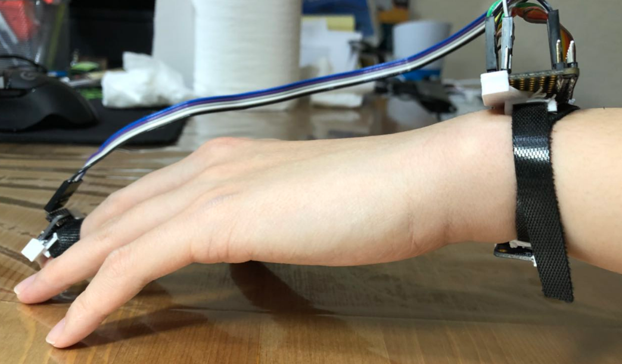
\includegraphics[width=.9\linewidth]{sensor.png}
  \caption{The hand tremor sensor developed for this study.}
  \label{fig:sensor}
\end{figure}
%
\subsection{Experimental Protocol}
%
The study was conducted in a quiet laboratory environment at Texas A\&M University, College Station. During the experiments, participants were seated comfortably on a chair. All experimental procedures were performed by adequately trained staff, in accordance with the operating procedures. The participants wore an accelerometer fixed on the wrist and middle finger's terminal phalanx. The subjects were asked to estimate the intensity of exercises using the rated perceived exertion (RPE) scale ranging from 1 to 10 and whether their left- or right-hand is dominant. The experiment stopped when the participant declared that they were fatigued and could not continue further. Tremor was assessed in three stages.
%

In the first stage, pre-fatigue test ($\sim 3$ min), the rest, posture and isometric tremors were tested in rest, unloaded posture and loaded posture positions, respectively. In the rest position, the participant's forearm was completely underlaid and the hand and fingers were fully relaxed to avoid voluntary muscle activity in both-forearm and hand. In the condition of posture, the participants raised the dominant arm horizontally in front of them, parallel to the floor by keeping \SI{90}{\degree} angle between the body and arm, the arm in the elbow and fingers are stretched out. In the loaded posture condition, the postural tremor when participants, holding 300 g weight (Jamar Hydraulic Hand Dynamometer) in the distal half of their horizontally extended hand, was measured. Each exercise was with duration 15 s followed by 30 s rest.

\begin{figure*}[h!]
	\centering
	\subfloat[Finger - PC]{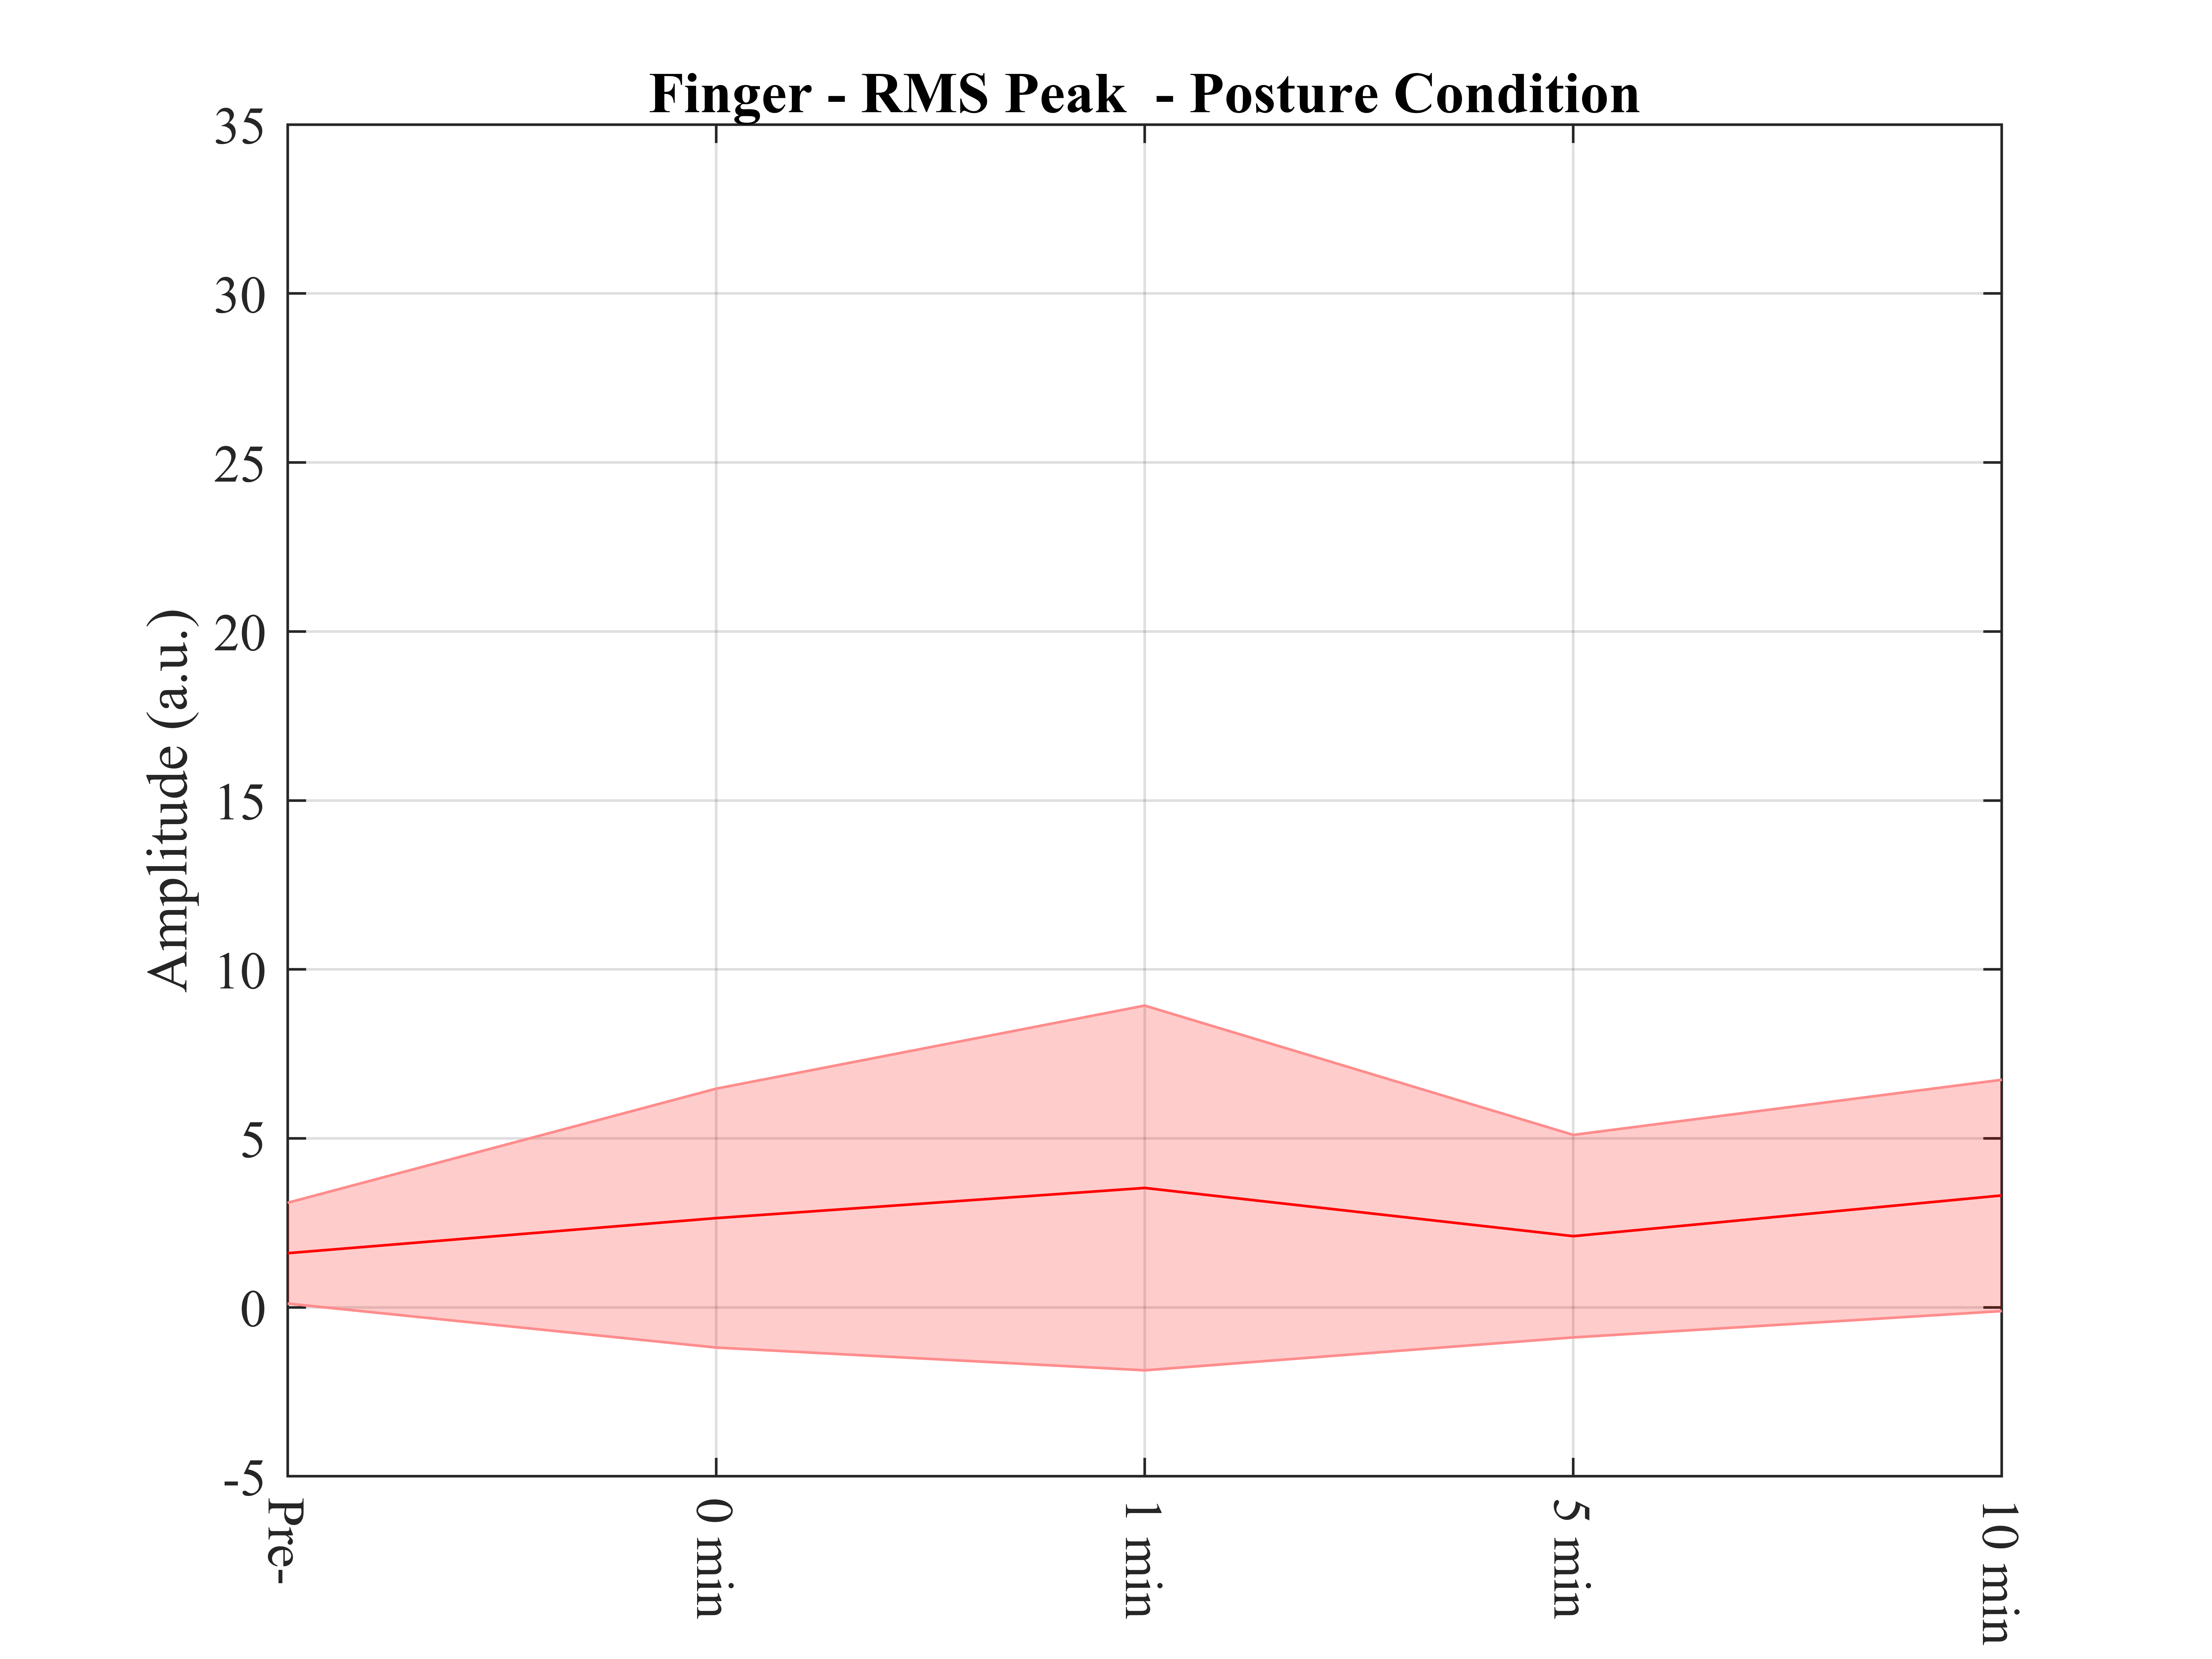
\includegraphics[width=0.31\textwidth]{Figures/finger_Posture_condition-rms_peak_shaded.tex}}
	\label{fig:finger_PC}
	\hfill
	\subfloat[Finger - RC]{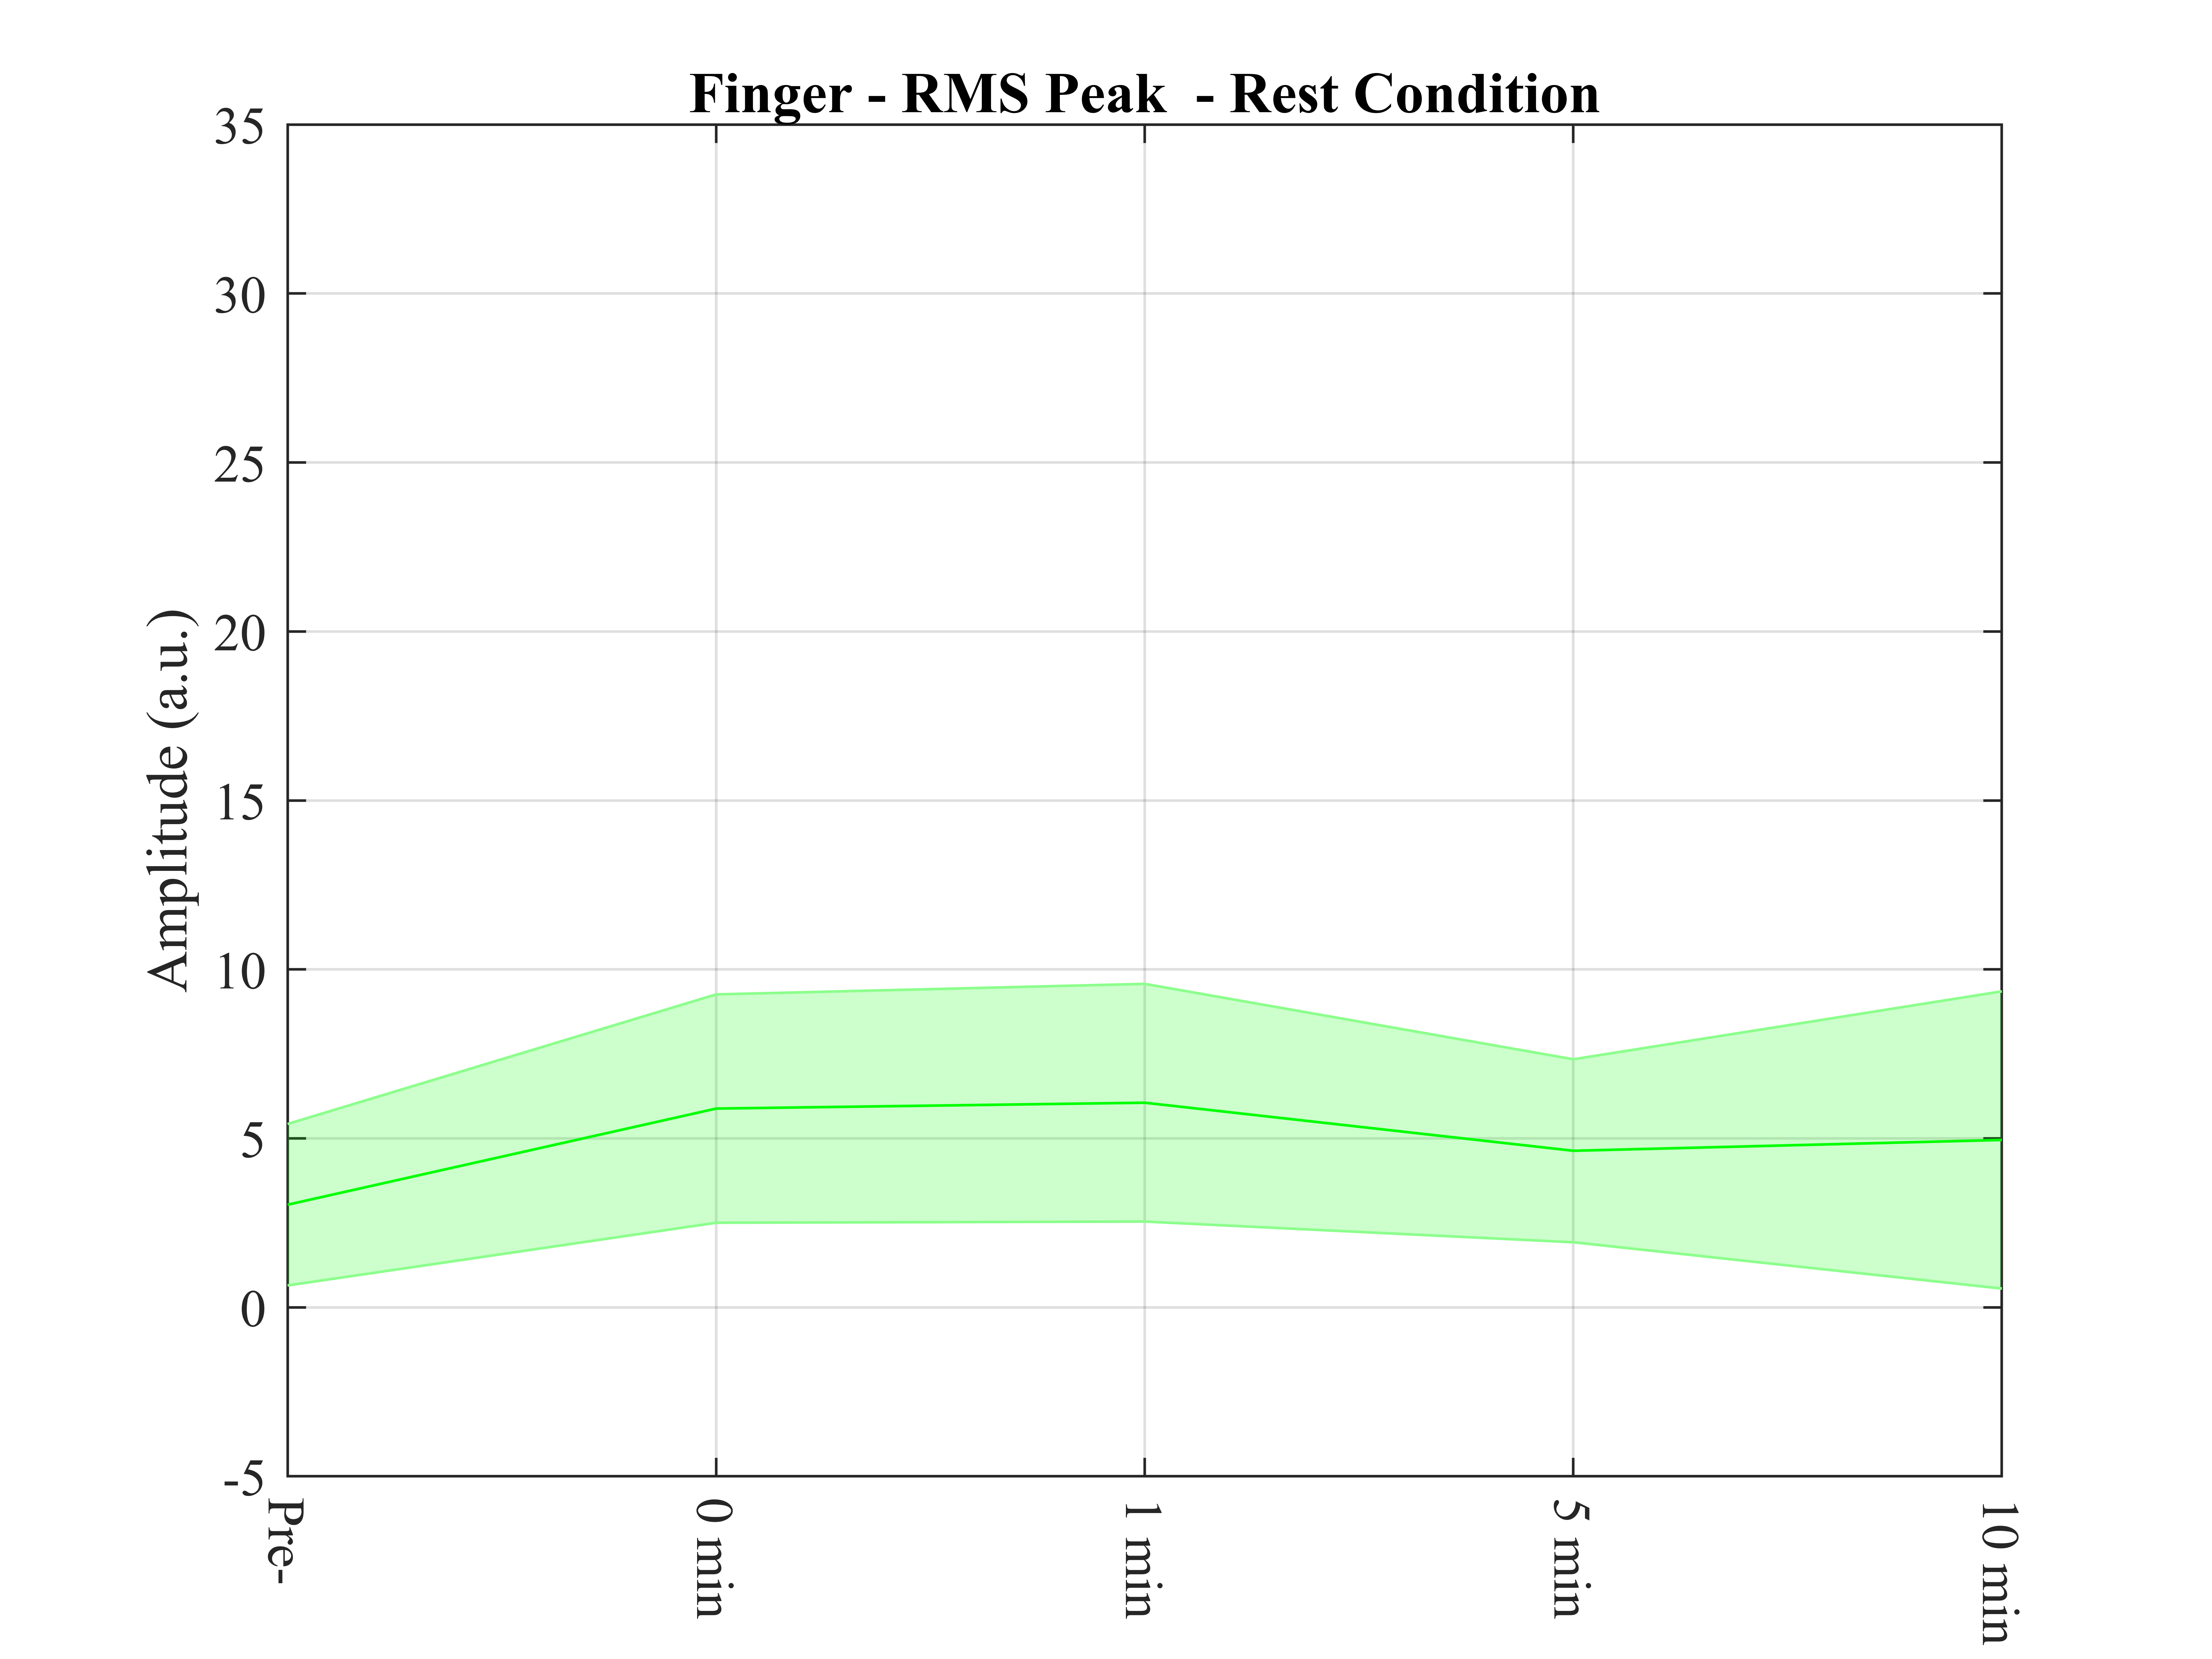
\includegraphics[width=0.31\textwidth]{Figures/finger_Rest_condition-rms_peak_shaded.tex}}
	\label{fig:finger_RC}
	\hfill
	\subfloat[Finger - LPC]{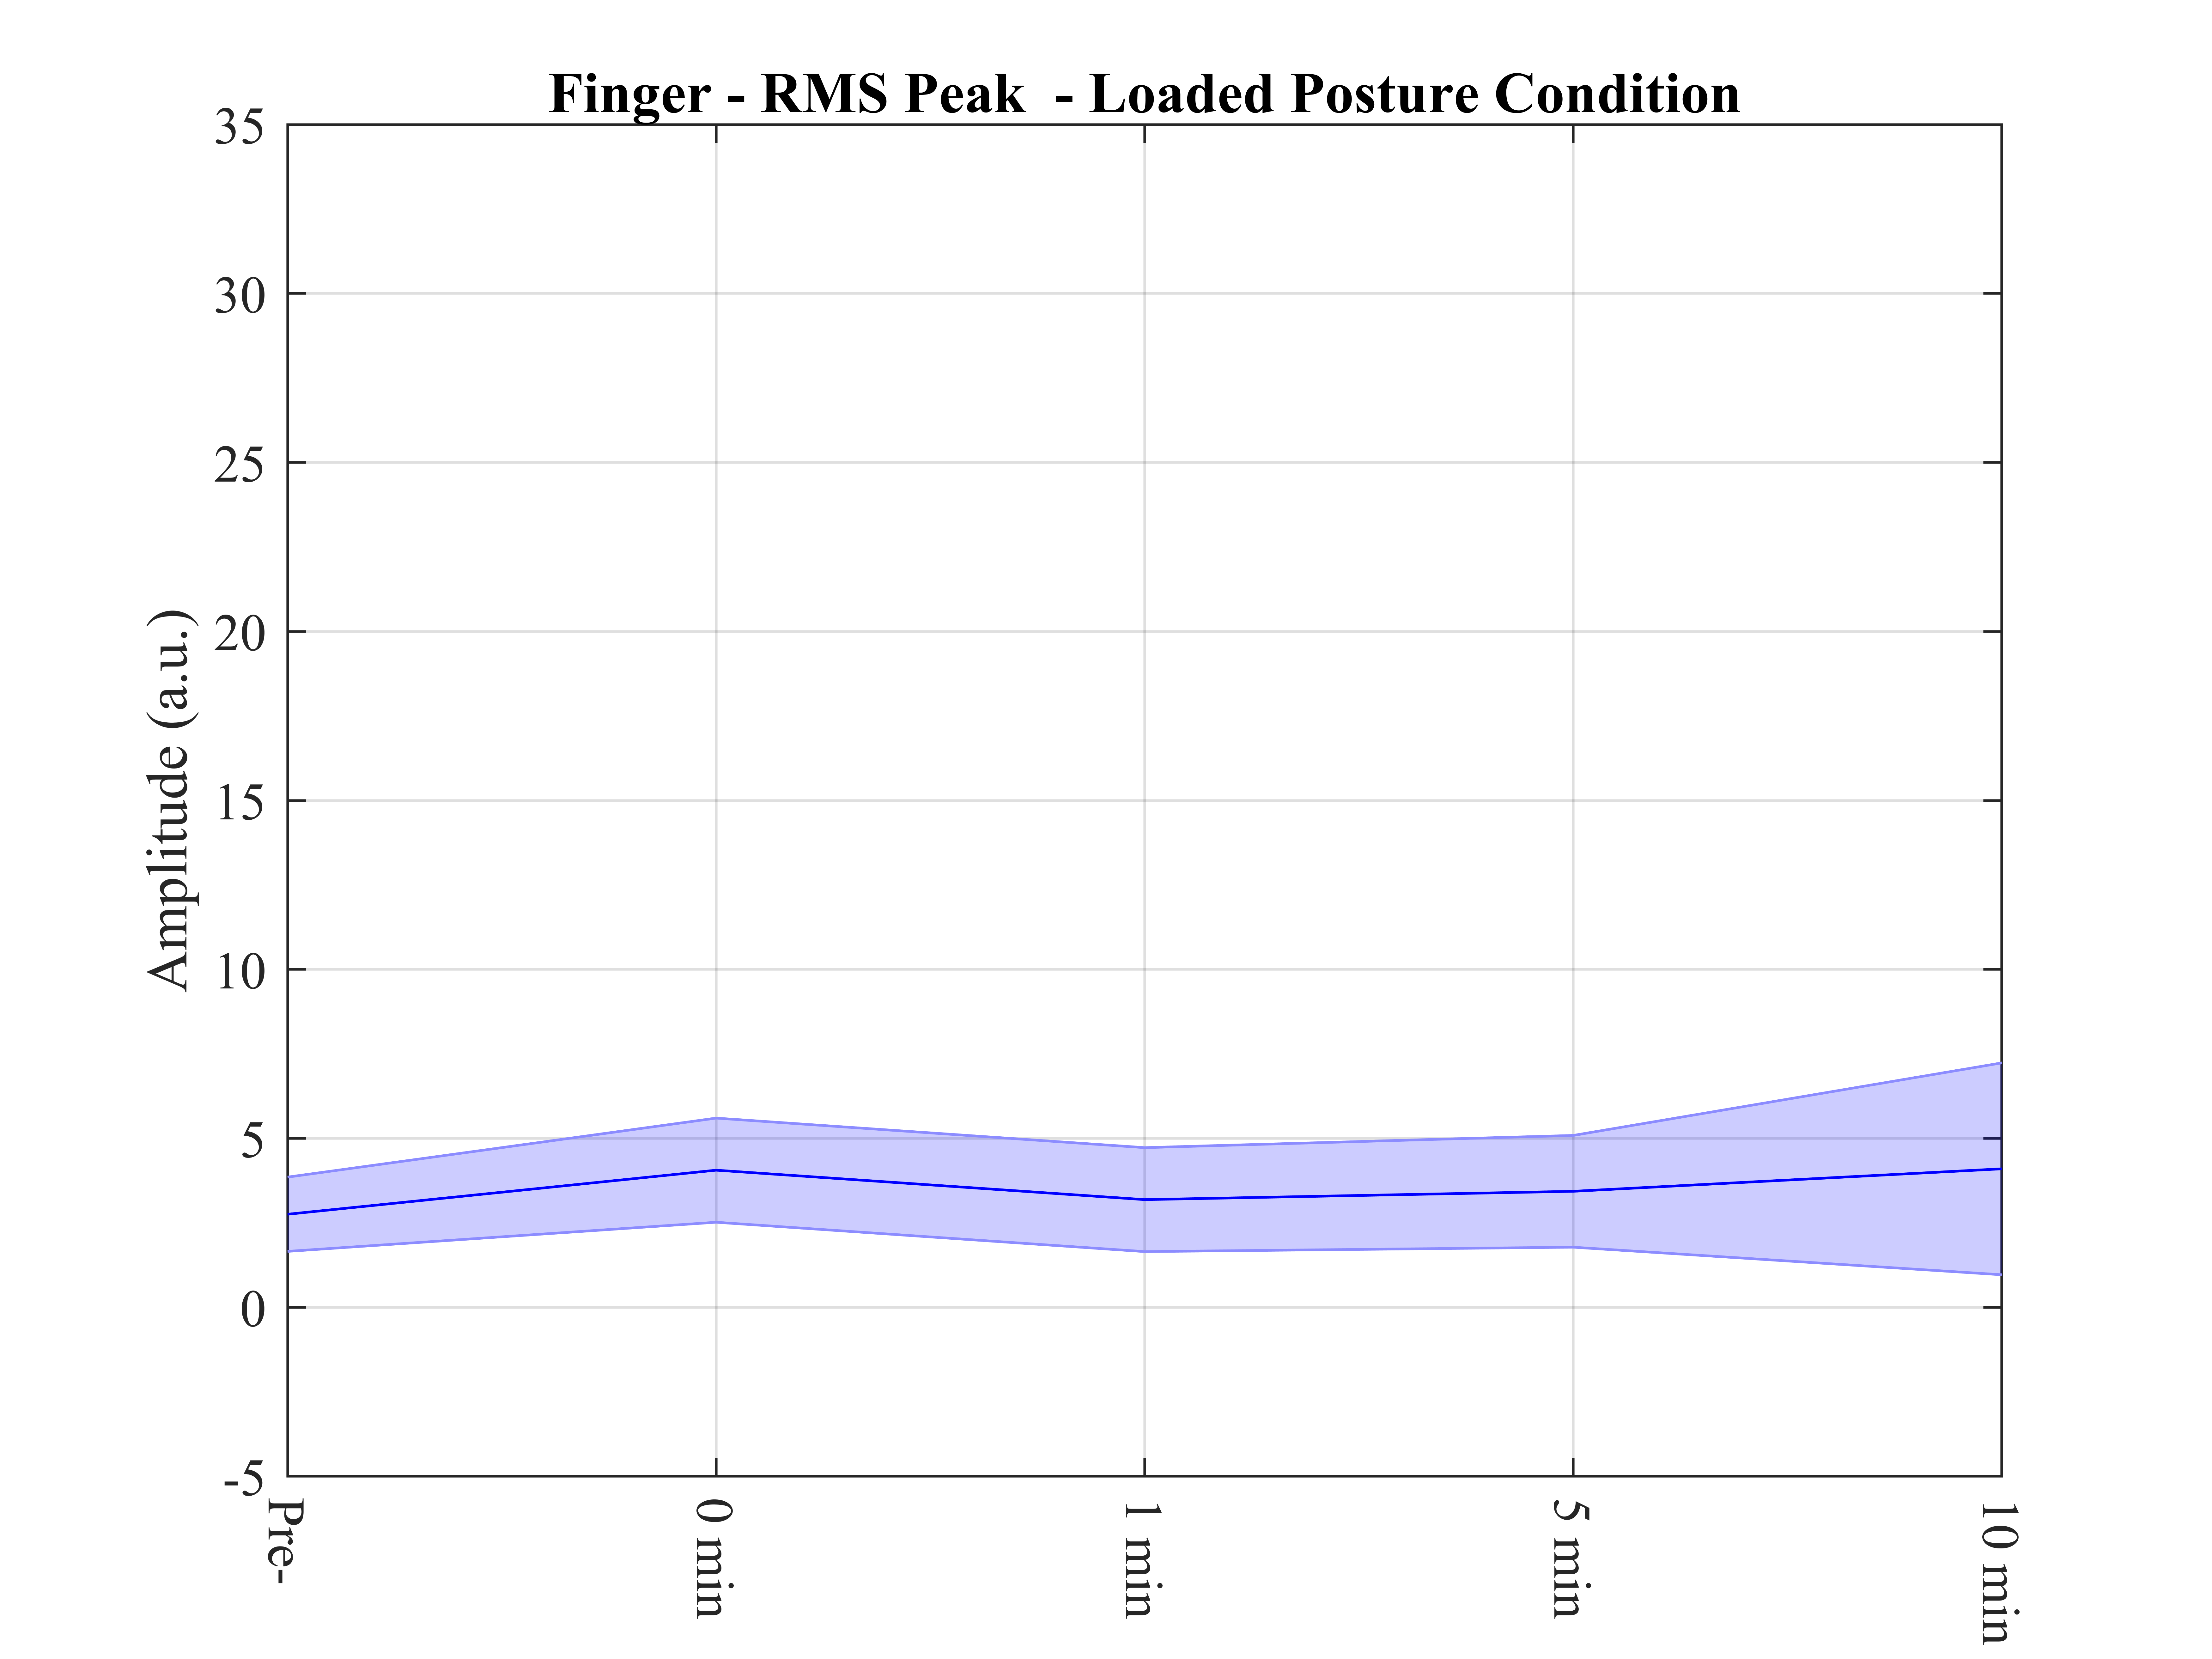
\includegraphics[width=0.31\textwidth]{Figures/finger_loaded_condition-rms_peak_shaded.tex}}
	\label{fig:finger_LPC}
	\medskip
  \subfloat[Wrist - PC]{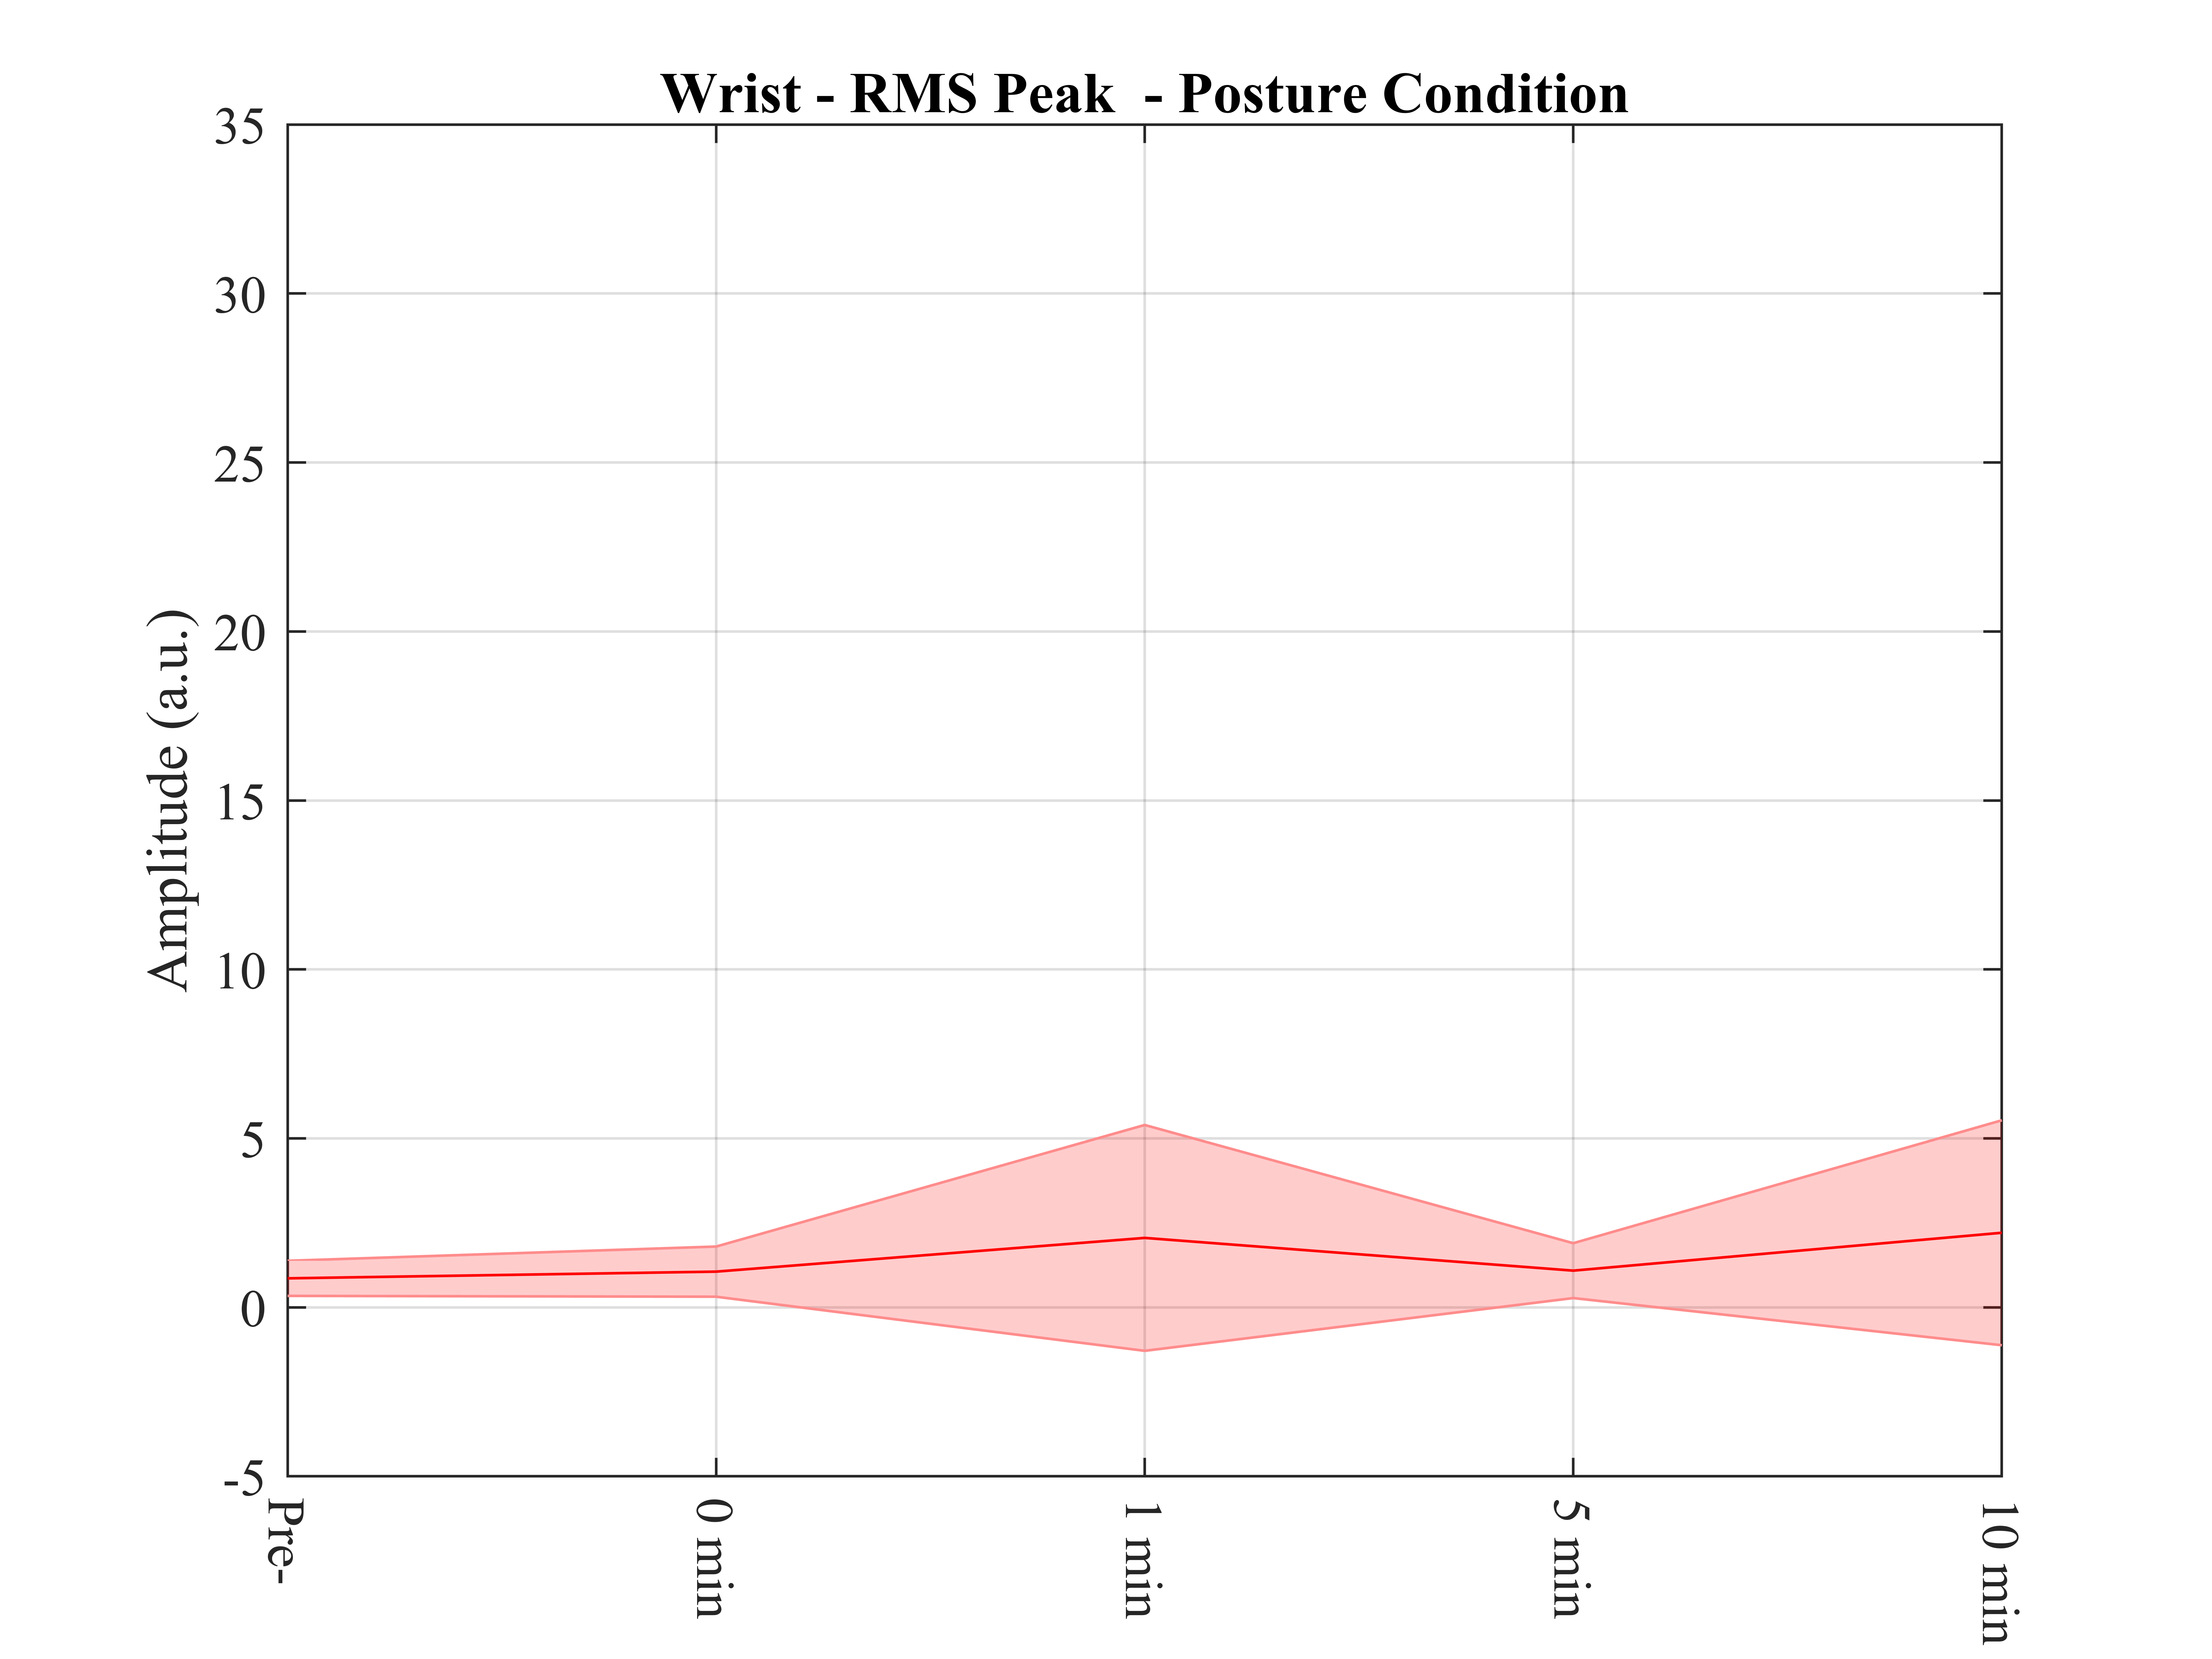
\includegraphics[width=0.31\textwidth]{Figures/wrist_Posture_condition-rms_peak_shaded_fatigued.tex}}
  \label{fig:wrist_PC}
  \hfill
  \subfloat[Wrist - RC]{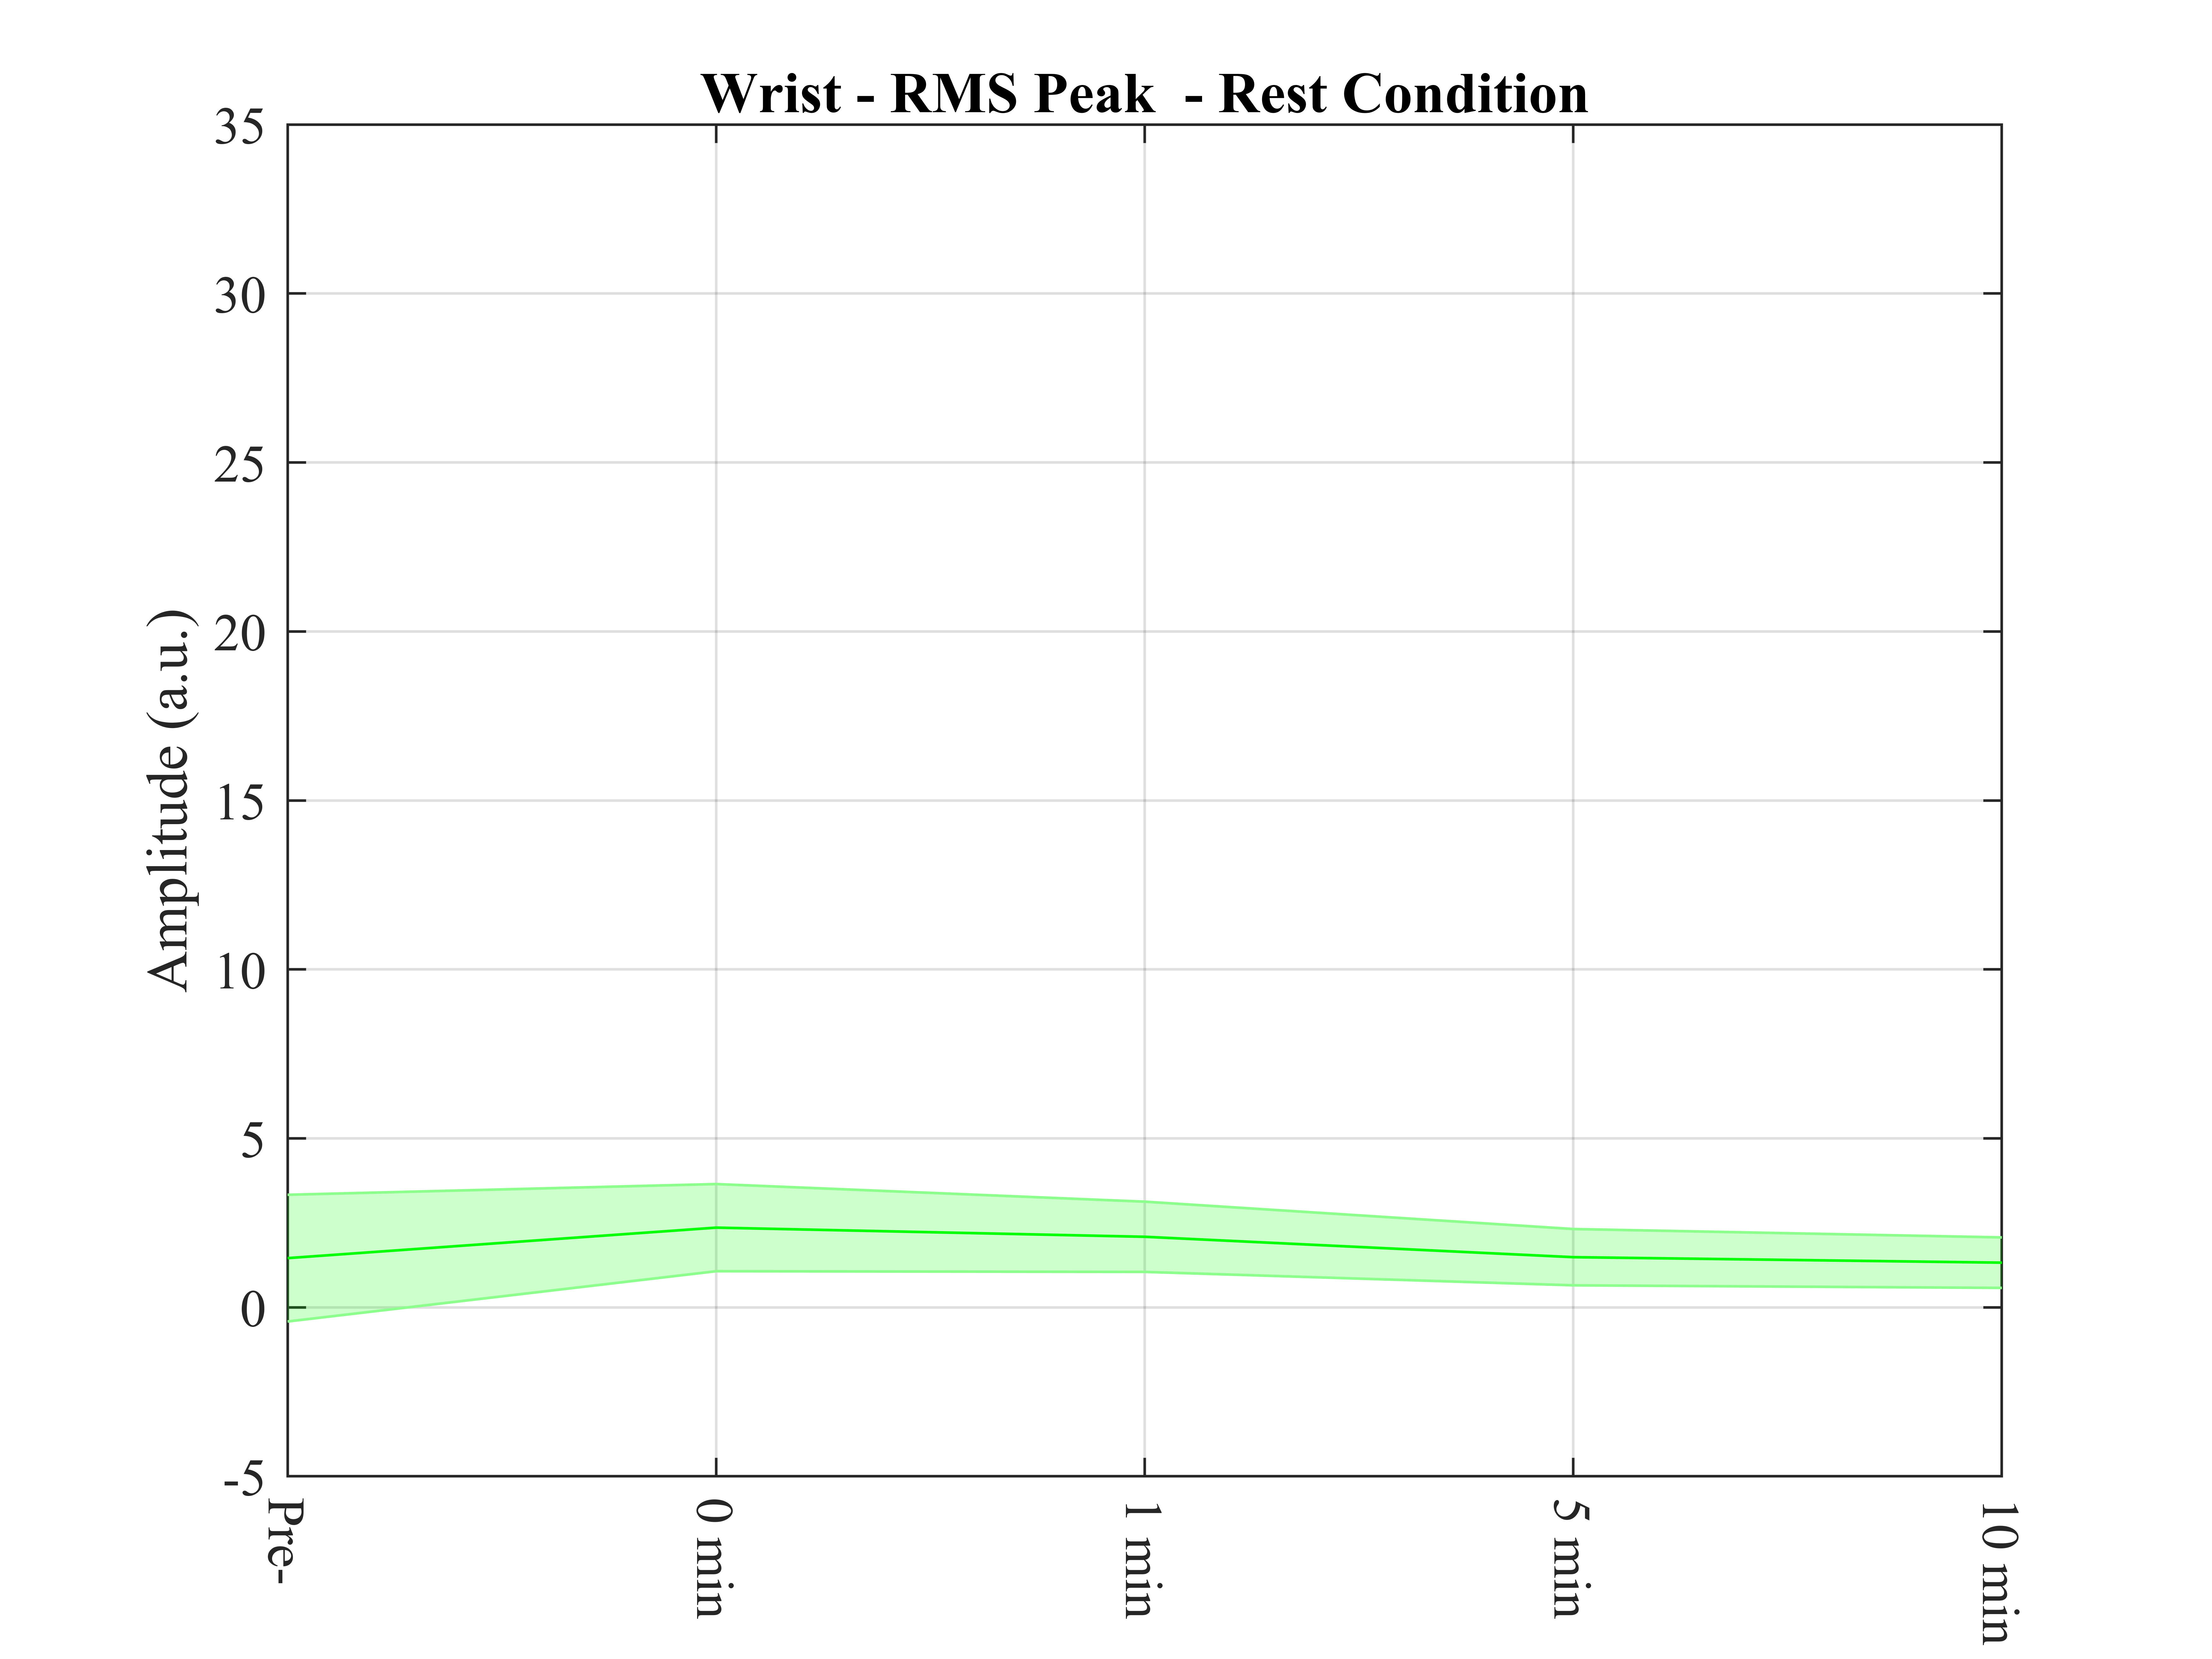
\includegraphics[width=0.31\textwidth]{Figures/wrist_Rest_condition-rms_peak_shaded_fatigued.tex}}
  \label{fig:wrist_RC}
  \hfill
  \subfloat[Wrist - LPC]{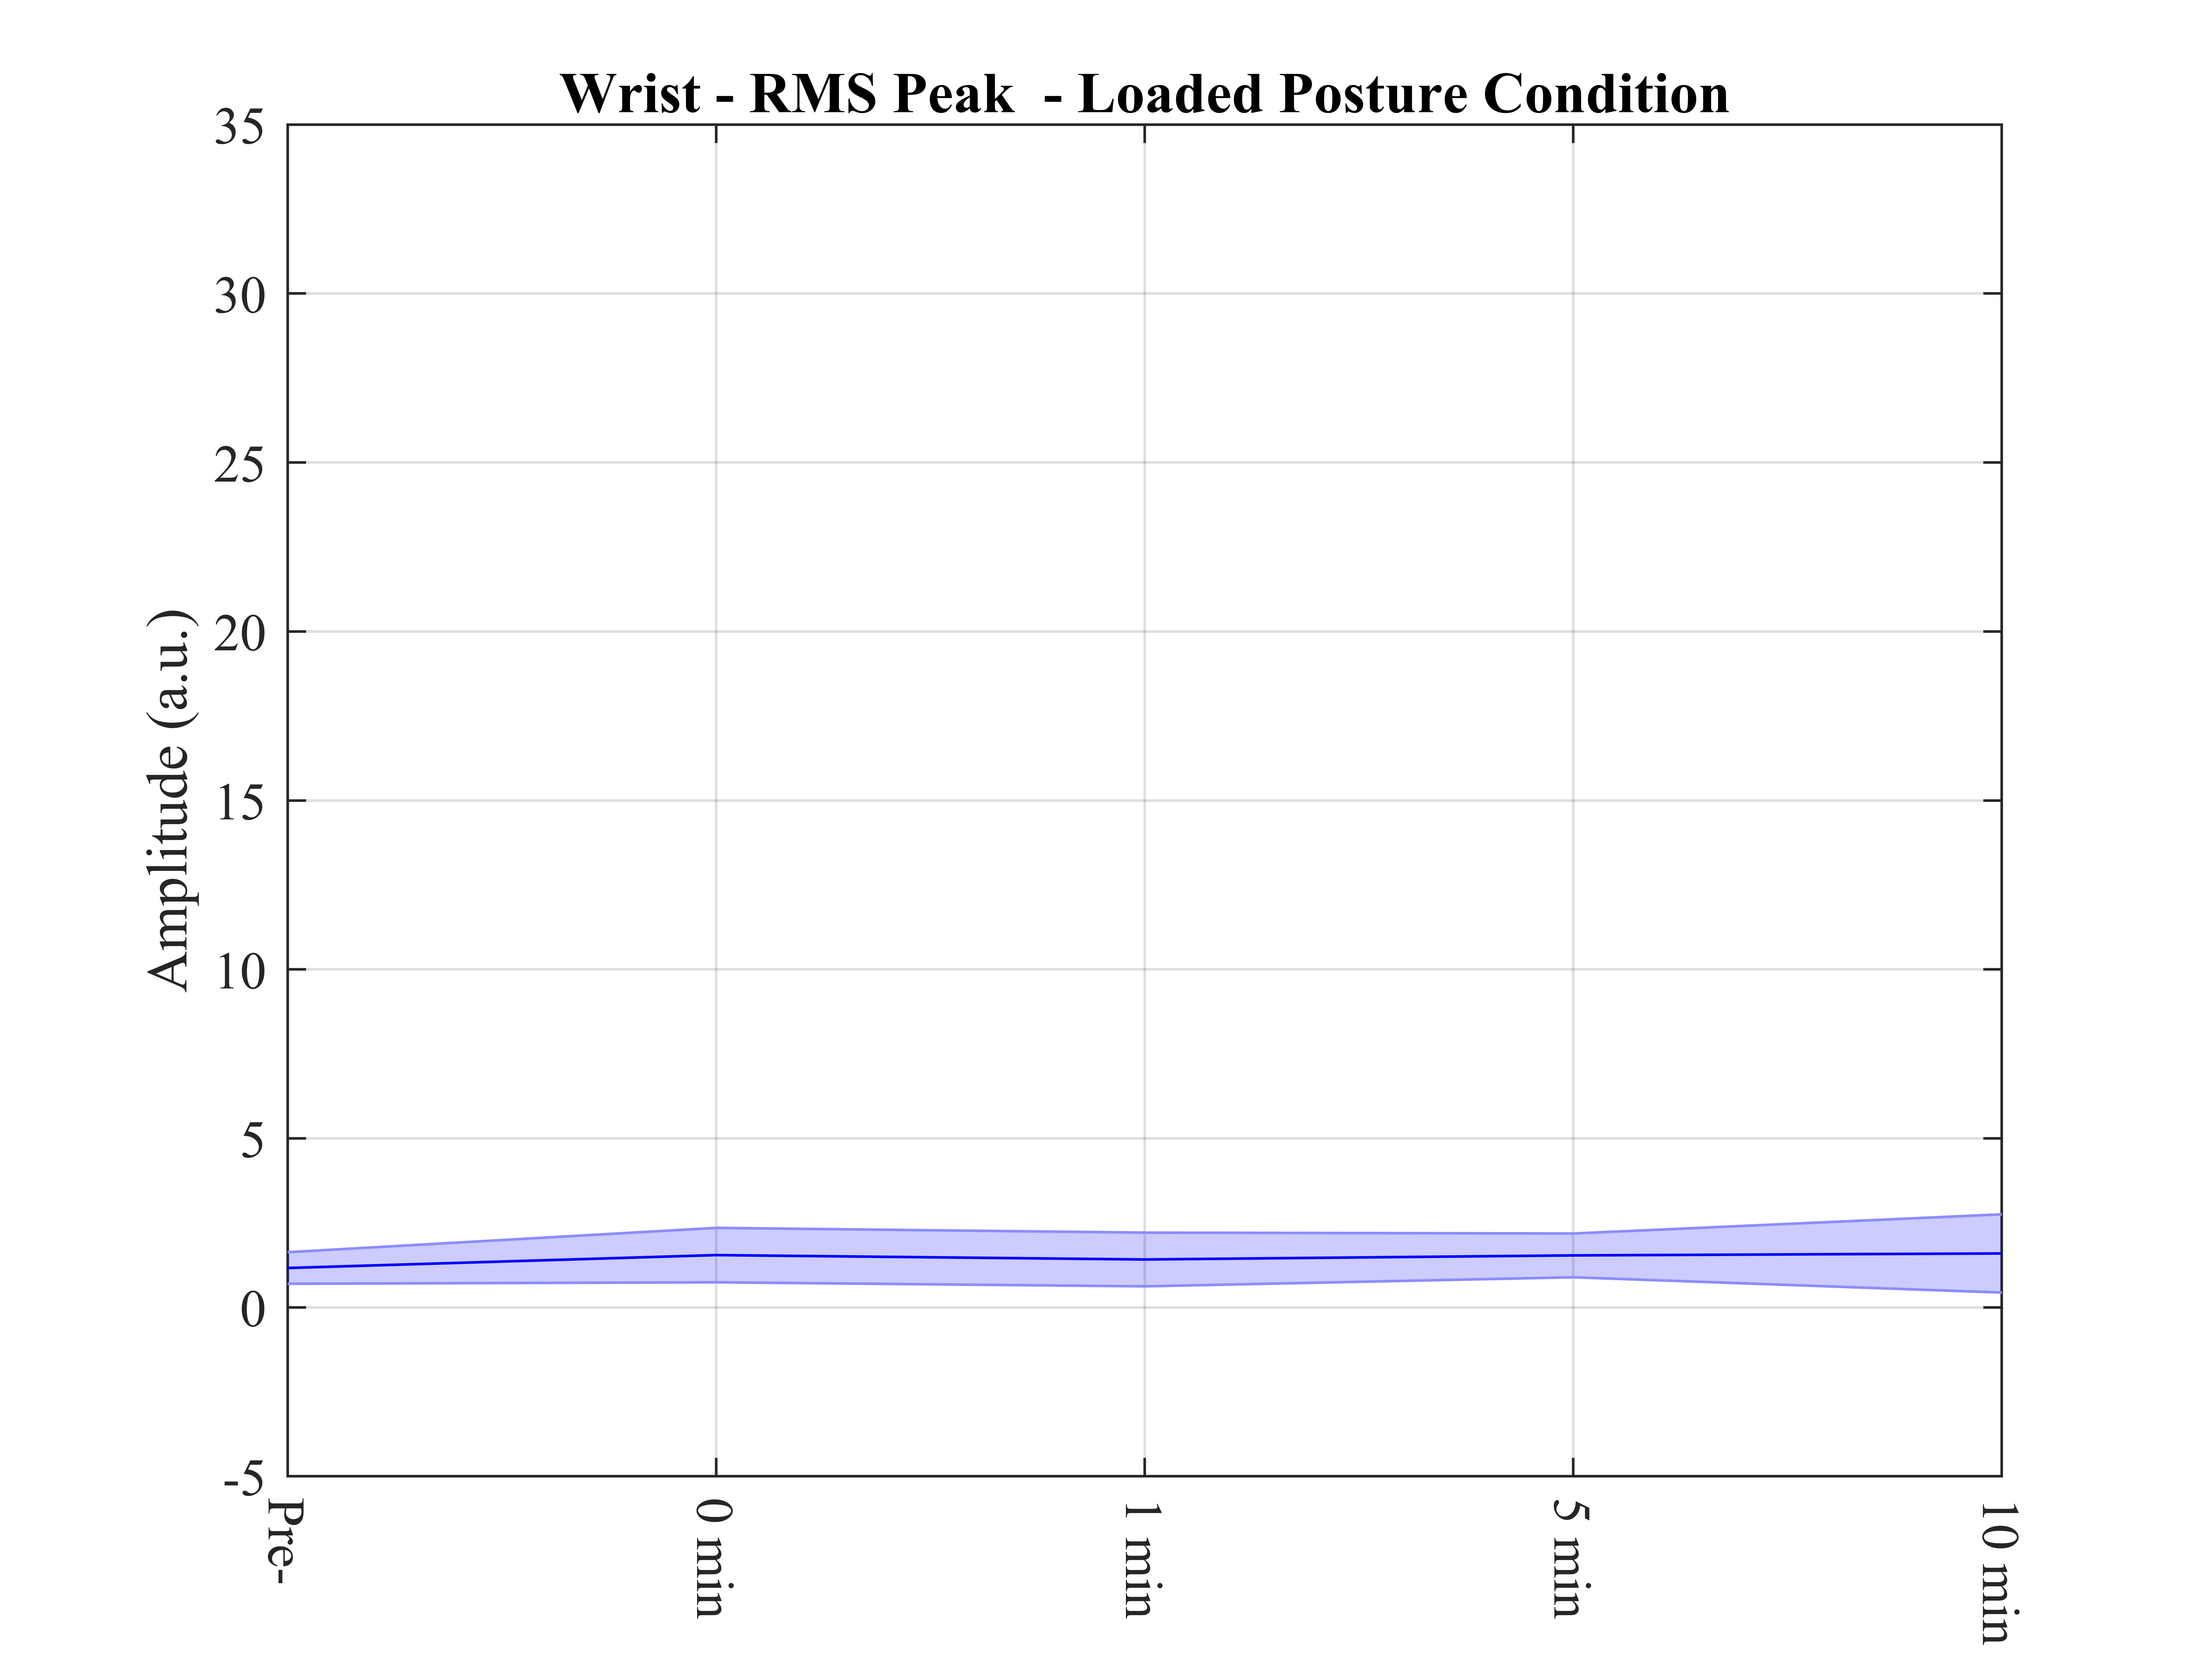
\includegraphics[width=0.31\textwidth]{Figures/wrist_loaded_condition-rms_peak_shaded_fatigued.tex}}
  \label{fig:wrist_LPC}
	\caption{RMS values of the different actions obtained from the finger and wrist}
	\label{fig:RMS}
\end{figure*}
% 
\begin{table*}[!h]
\centering
\caption{PSD Distribution of the physiologic tremor.}
\begin{tabular}{c c c c c c c c c c}
\toprule
{Sensor Location} & \multicolumn{9}{c}{PSD Distribution (\%)}{}{} \\
\cmidrule{2-10}
& \multicolumn{3}{c}{Rest Condition} & \multicolumn{3}{c}{Posture Condition} & \multicolumn{3}{c}{Loaded Posture Condition} \\
& {3-8 Hz} & {8-14 Hz} & {14-22 Hz} & {3-8 Hz} & {8-14 Hz} & {14-22 Hz} & {3-8 Hz} & {8-14 Hz} & {14-22 Hz} \\
\midrule \midrule
Finger & 48	& 30 & 18	& 49	& 26	& 19	& 54	& 24	& 18 \\
Wrist  & 38	& 34 & 	24 & 	41 & 30 &	30 &	30 &	34 &	31  \\
\bottomrule
\end{tabular}
\label{tab:features}
\end{table*}
% 
\begin{figure*}[!h]
	\centering
	\subfloat[Wrist - PC]{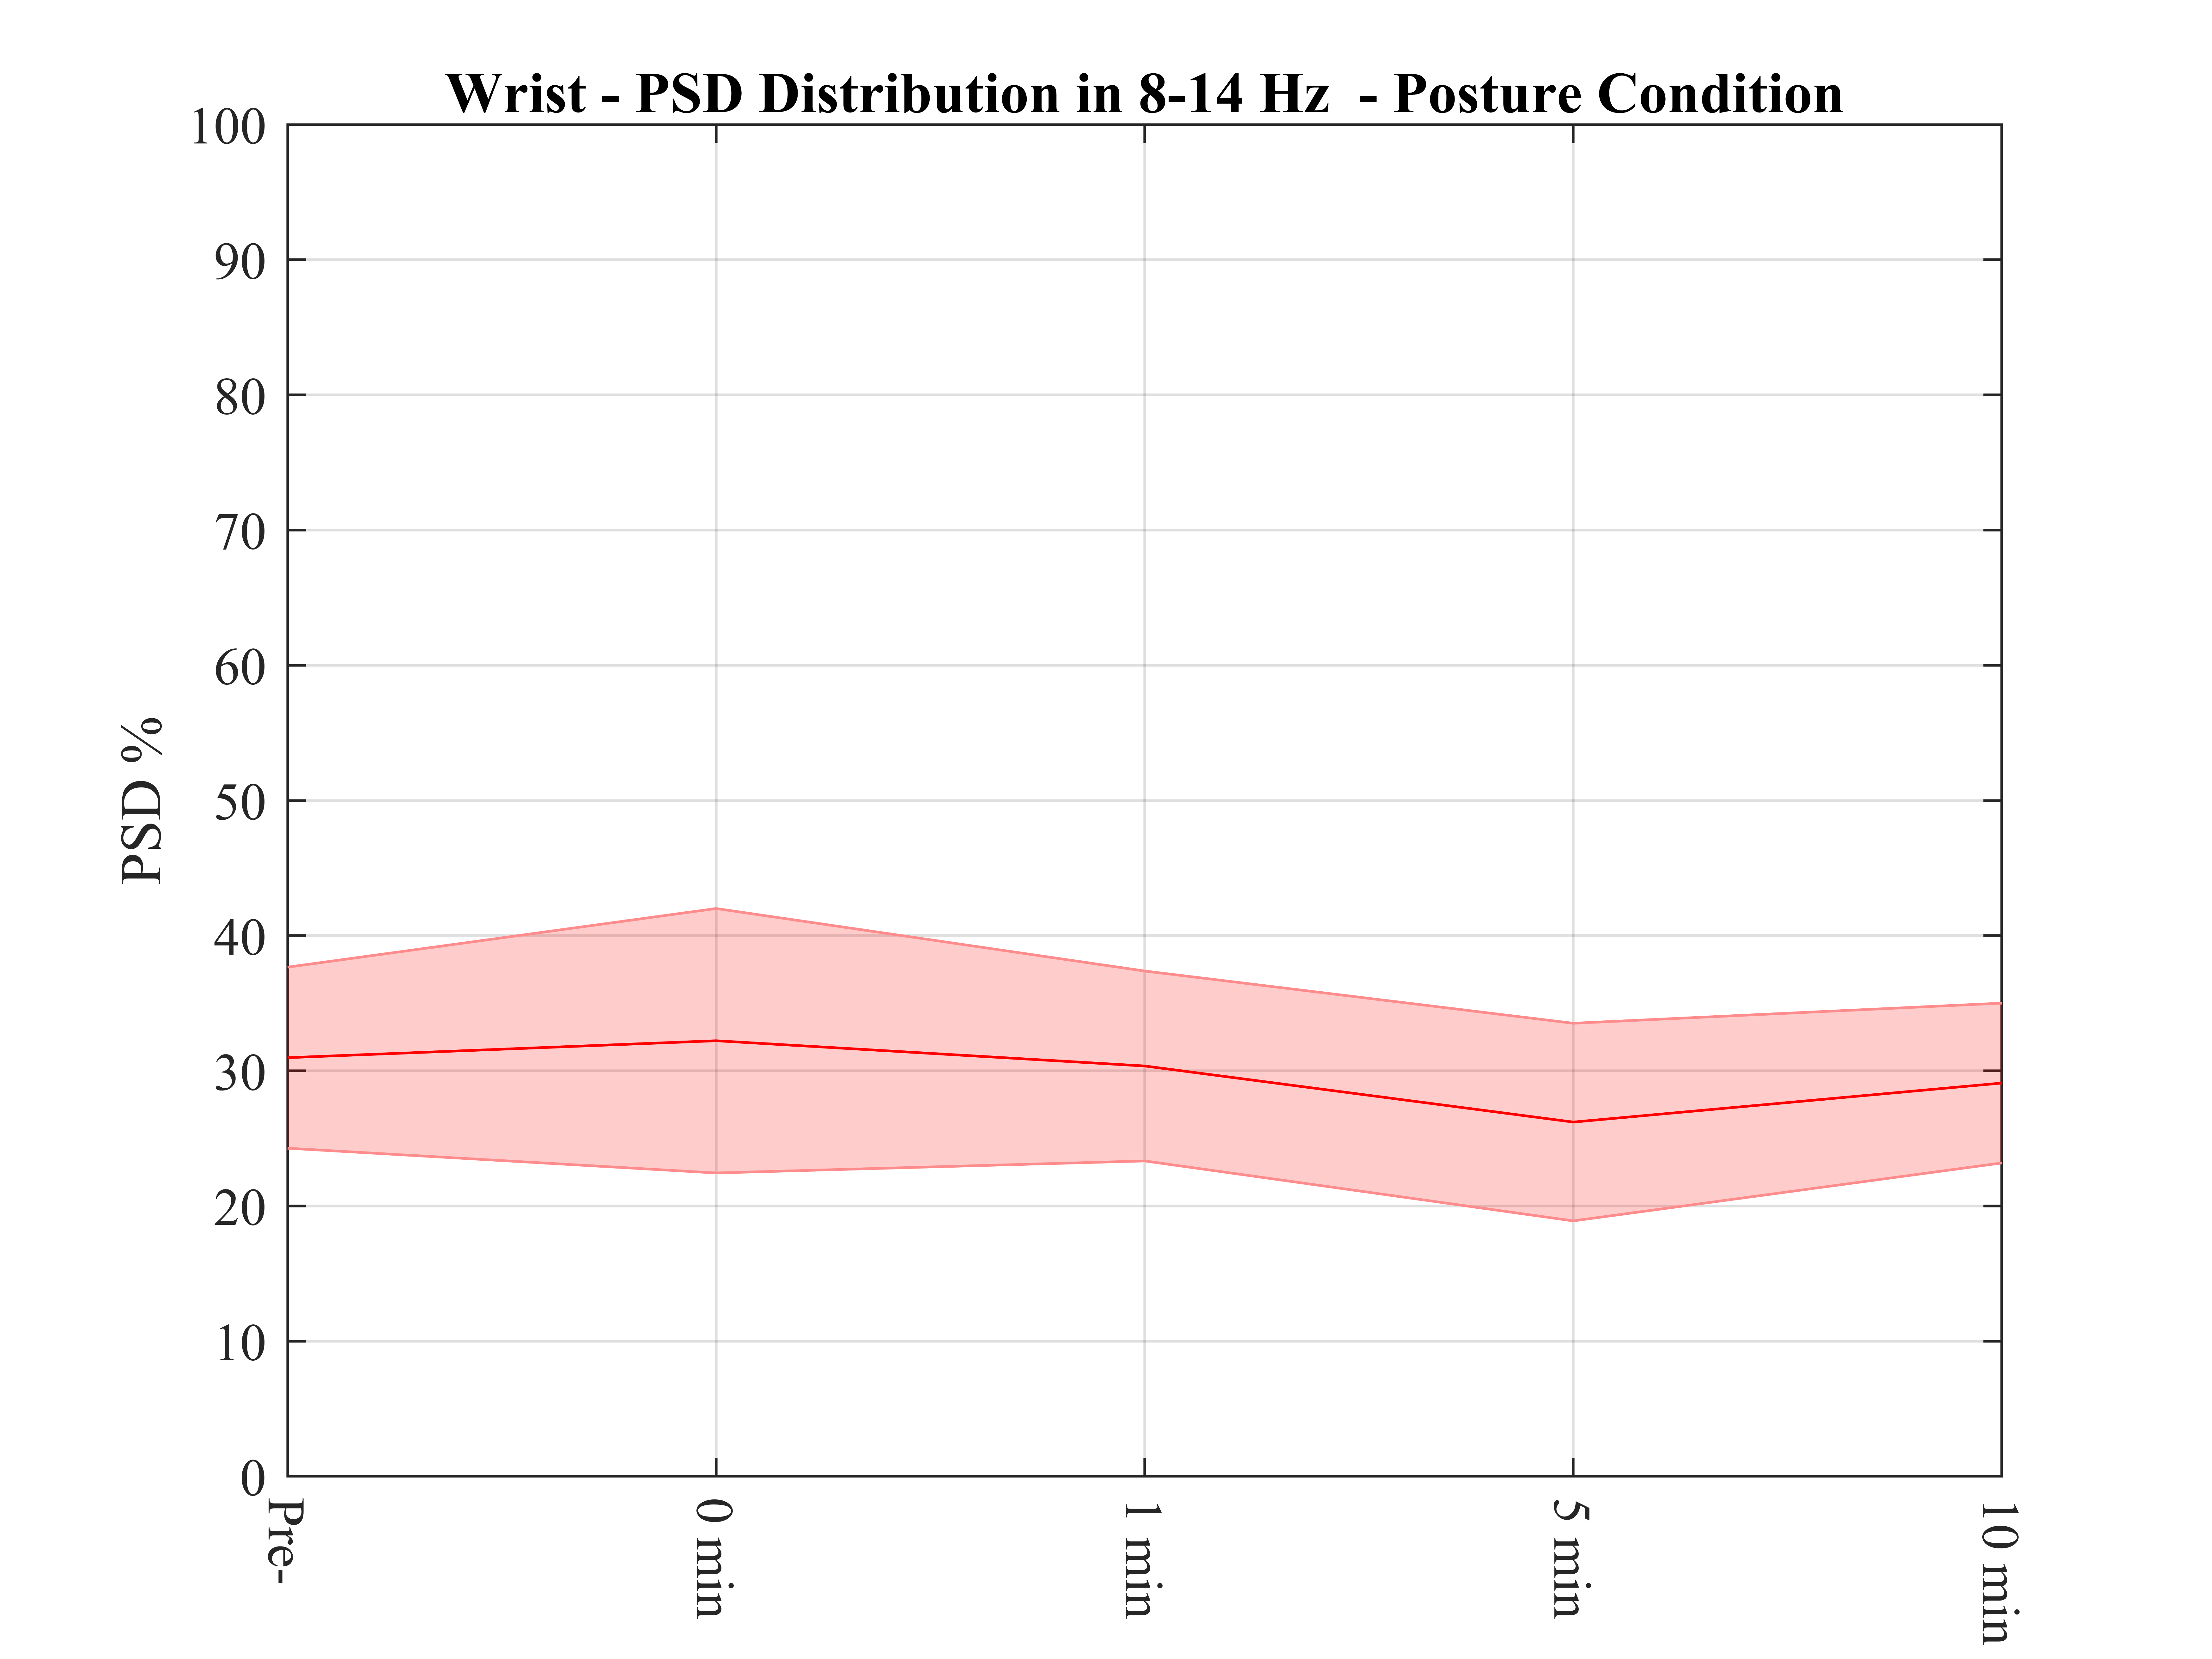
\includegraphics[width=0.31\textwidth]{Figures/wrist_Posture_condition-ept_shaded_8_14.tex}}
	\label{fig:wrist_PC_PSD}
	\hfill
	\subfloat[Wrist - RC]{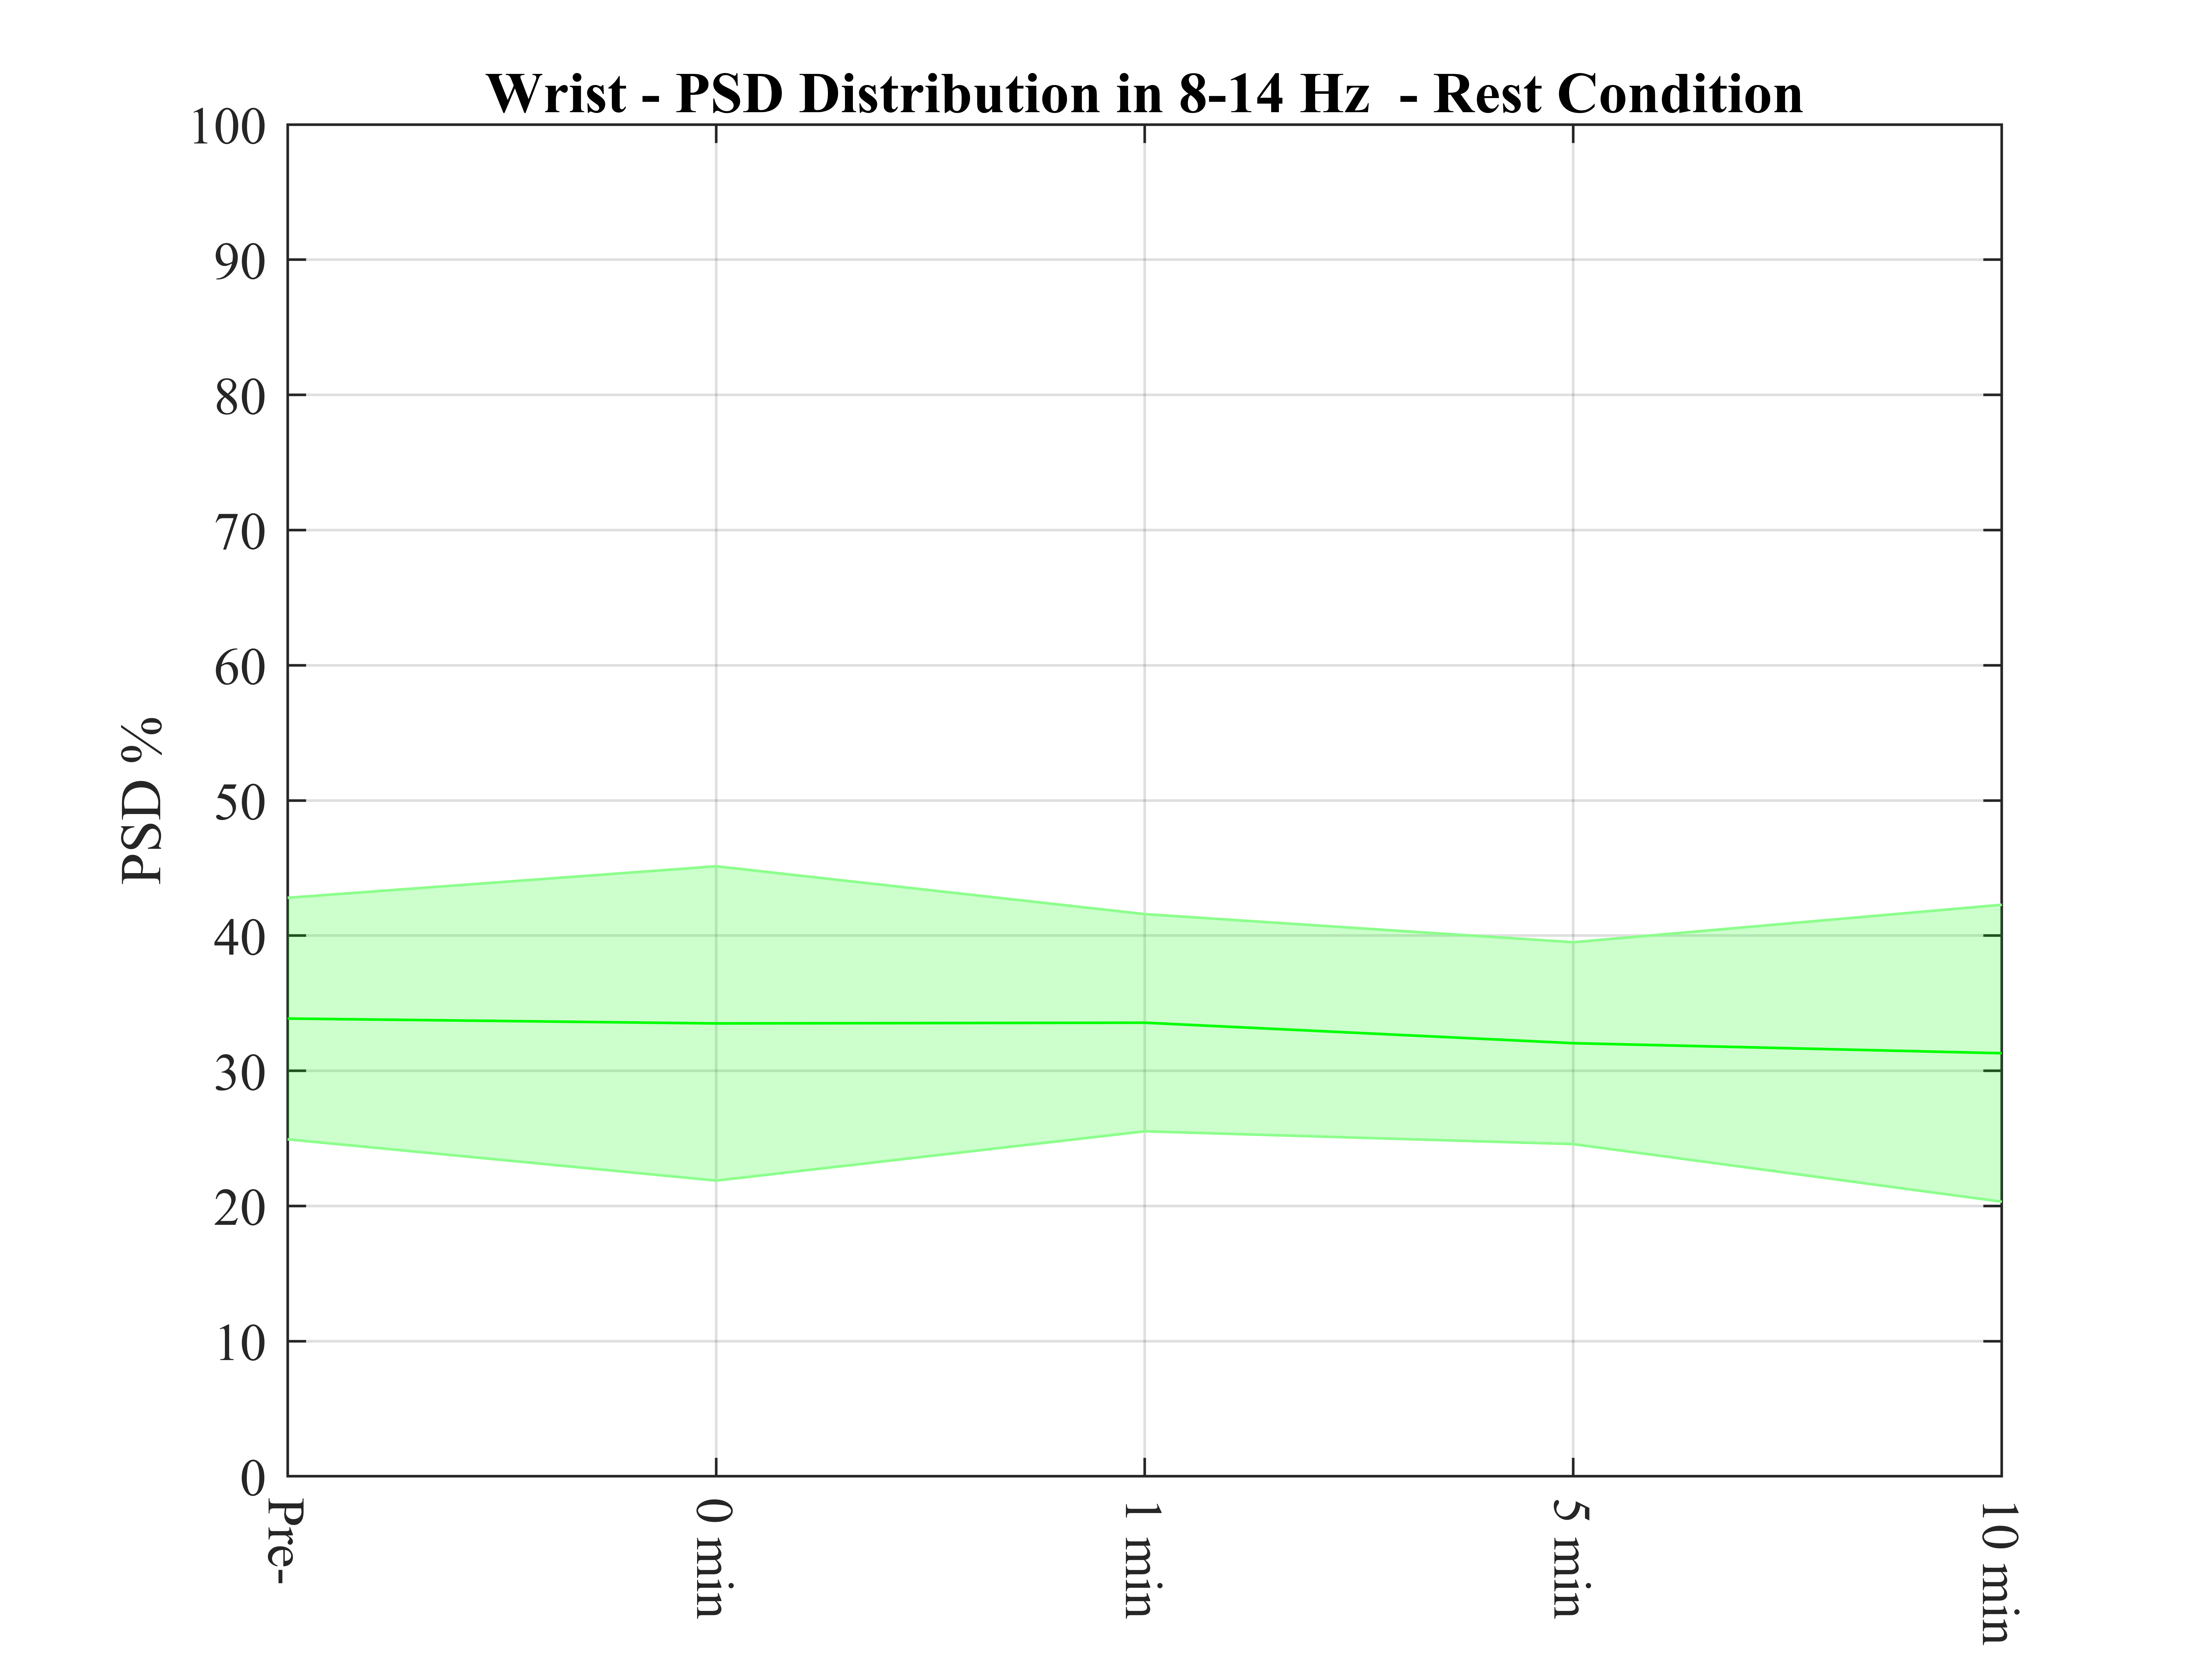
\includegraphics[width=0.31\textwidth]{Figures/wrist_Rest_condition-ept_shaded_8_14.tex}}
	\label{fig:wrist_RC_PSD}
	\hfill
	\subfloat[Wrist - LPC]{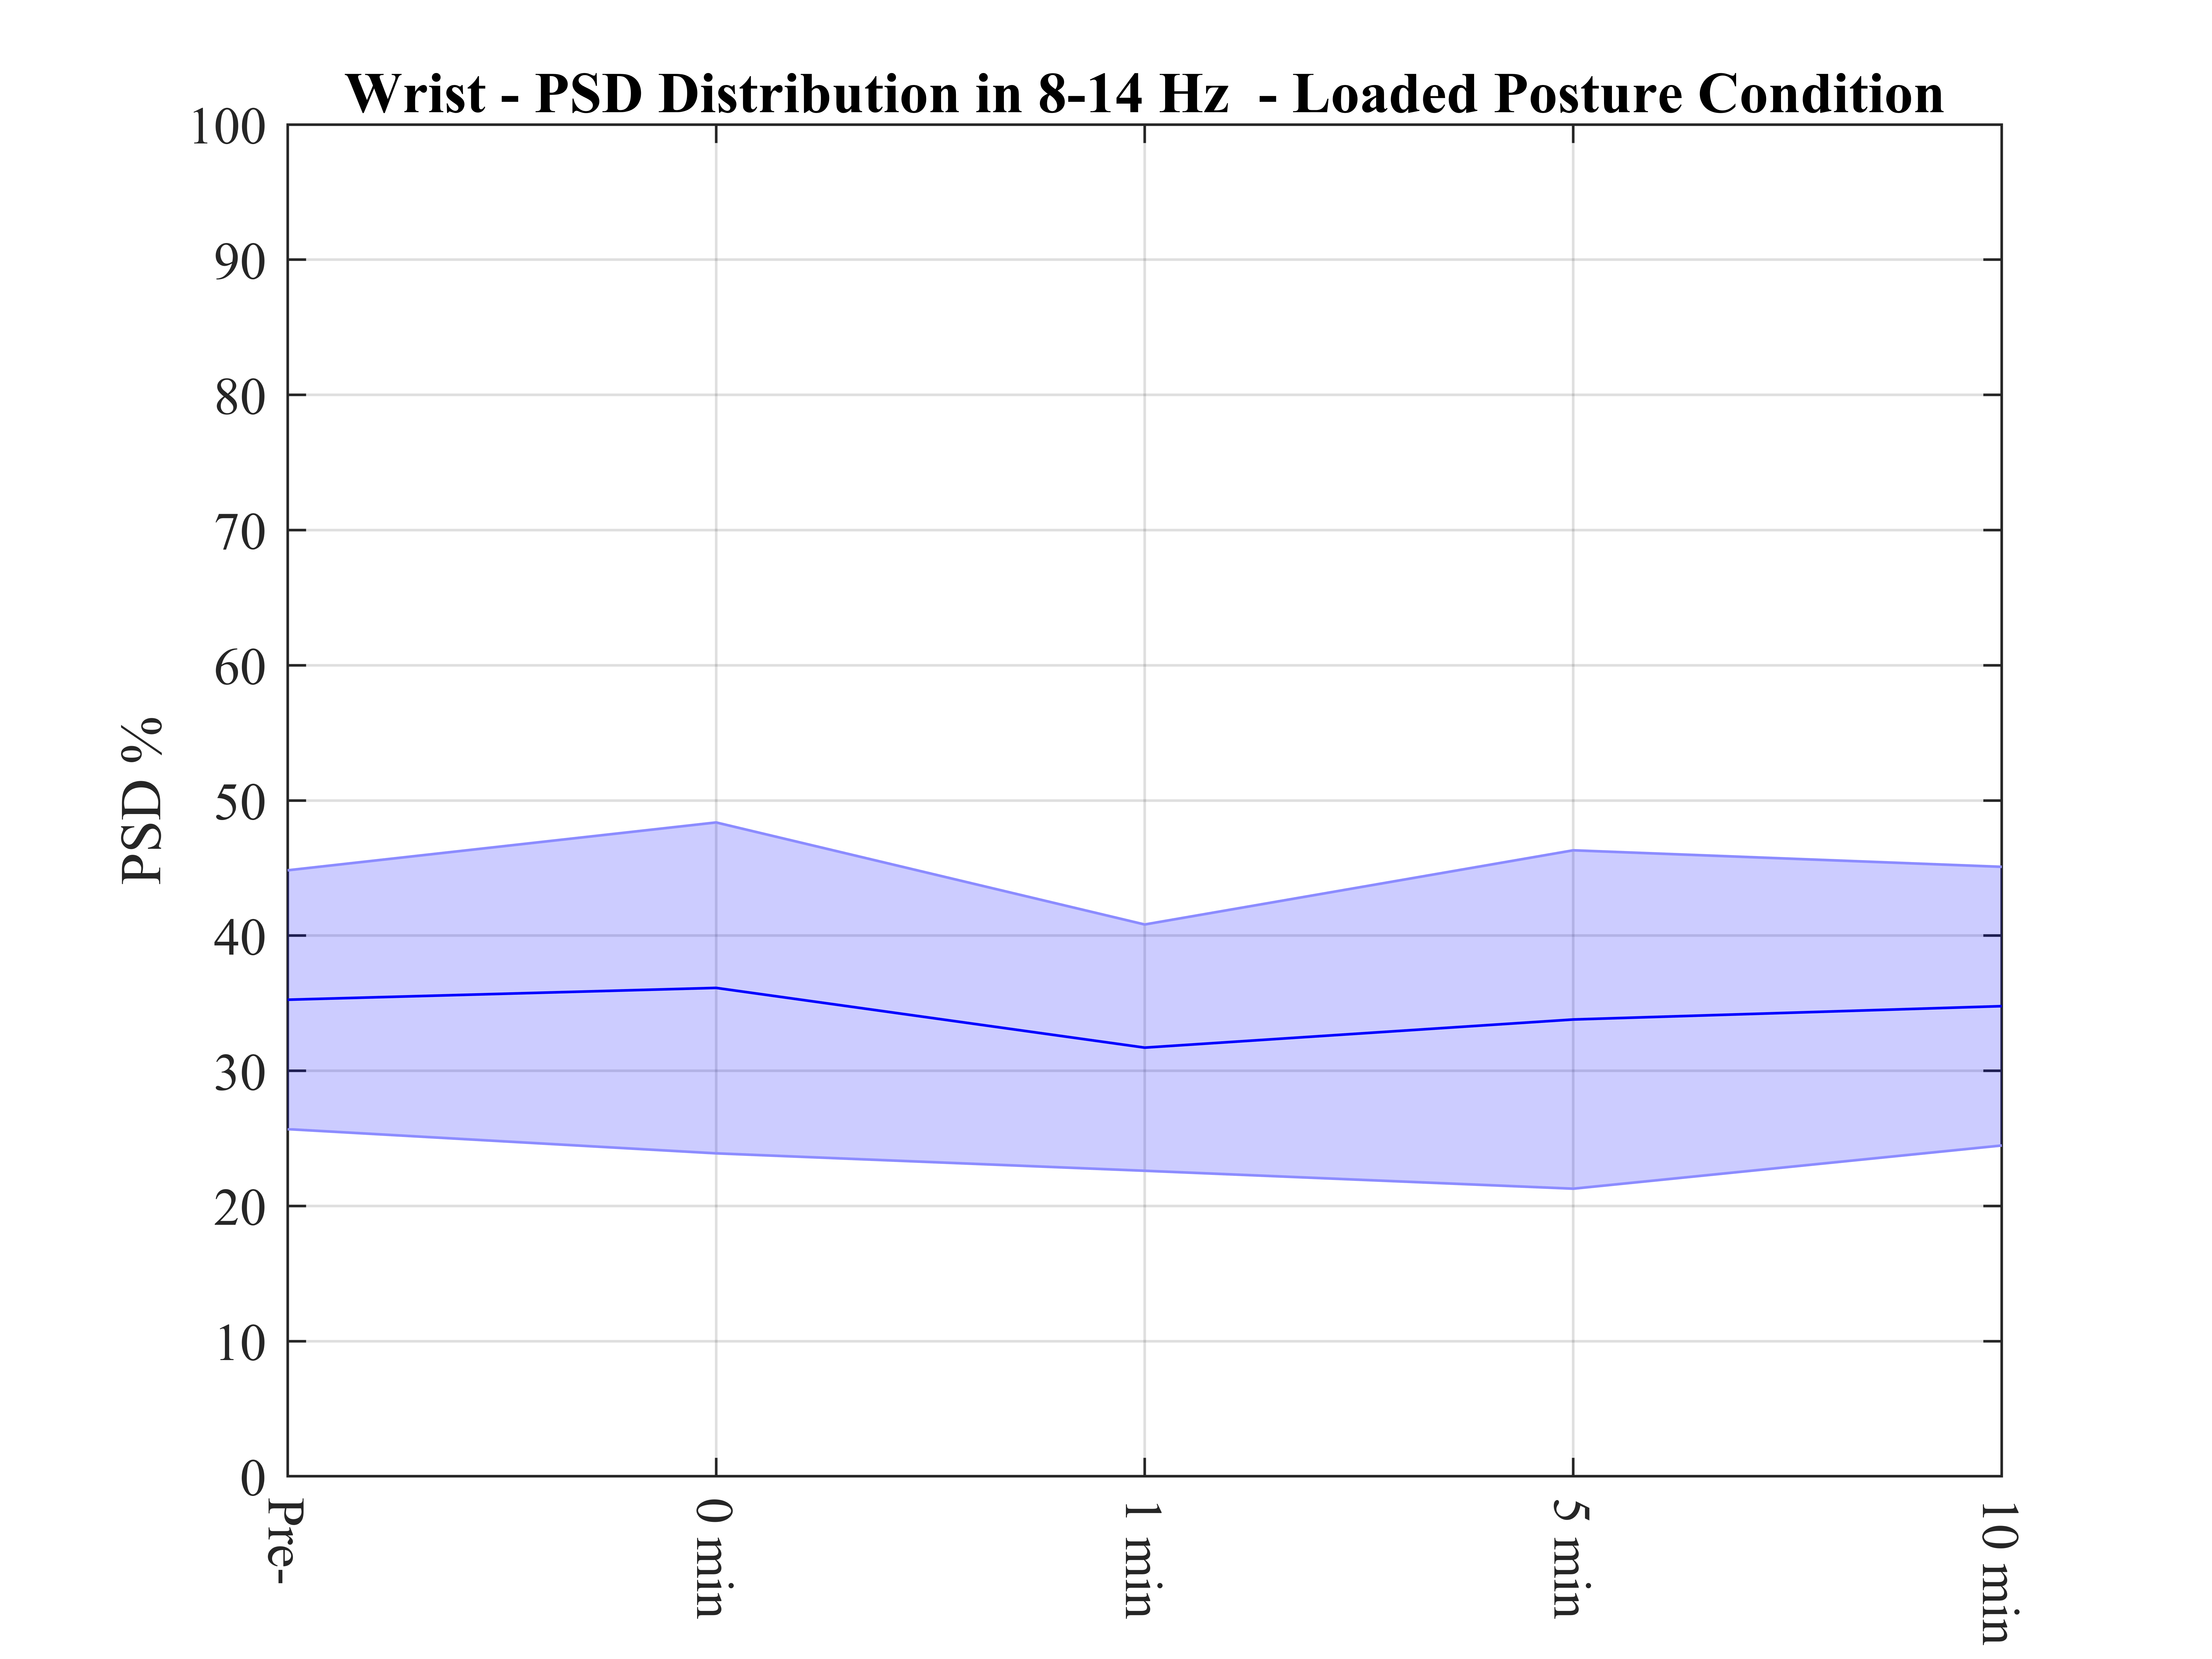
\includegraphics[width=0.31\textwidth]{Figures/wrist_loaded_condition-ept_shaded_8_14.tex}}
	\label{fig:wrist_LPC_PSD}
	\caption{PSD values of the different actions obtained from the wrist in the 8-14 Hz range}
	\label{fig:PSD}
\end{figure*}

The second stage, fatigue test ($\sim 10$ min), started with pre-maximum voluntary contraction (pre-MVC) repeated 3 times in which each episode lasted about 5 s followed by a 60 s rest. To determine the pre-MVC, a hand dynamometer was used. The fatigue tasks, a sustained contraction at 30\% MVC, consisted of the repetition of 30\% MVC exertion (15 s) and 15 s rest. The RPE was performed every 4 minutes and at the end of exhaustion.

\begin{figure*}[!t]
	\centering
	\subfloat[Wrist: 3 - 8 Hz]{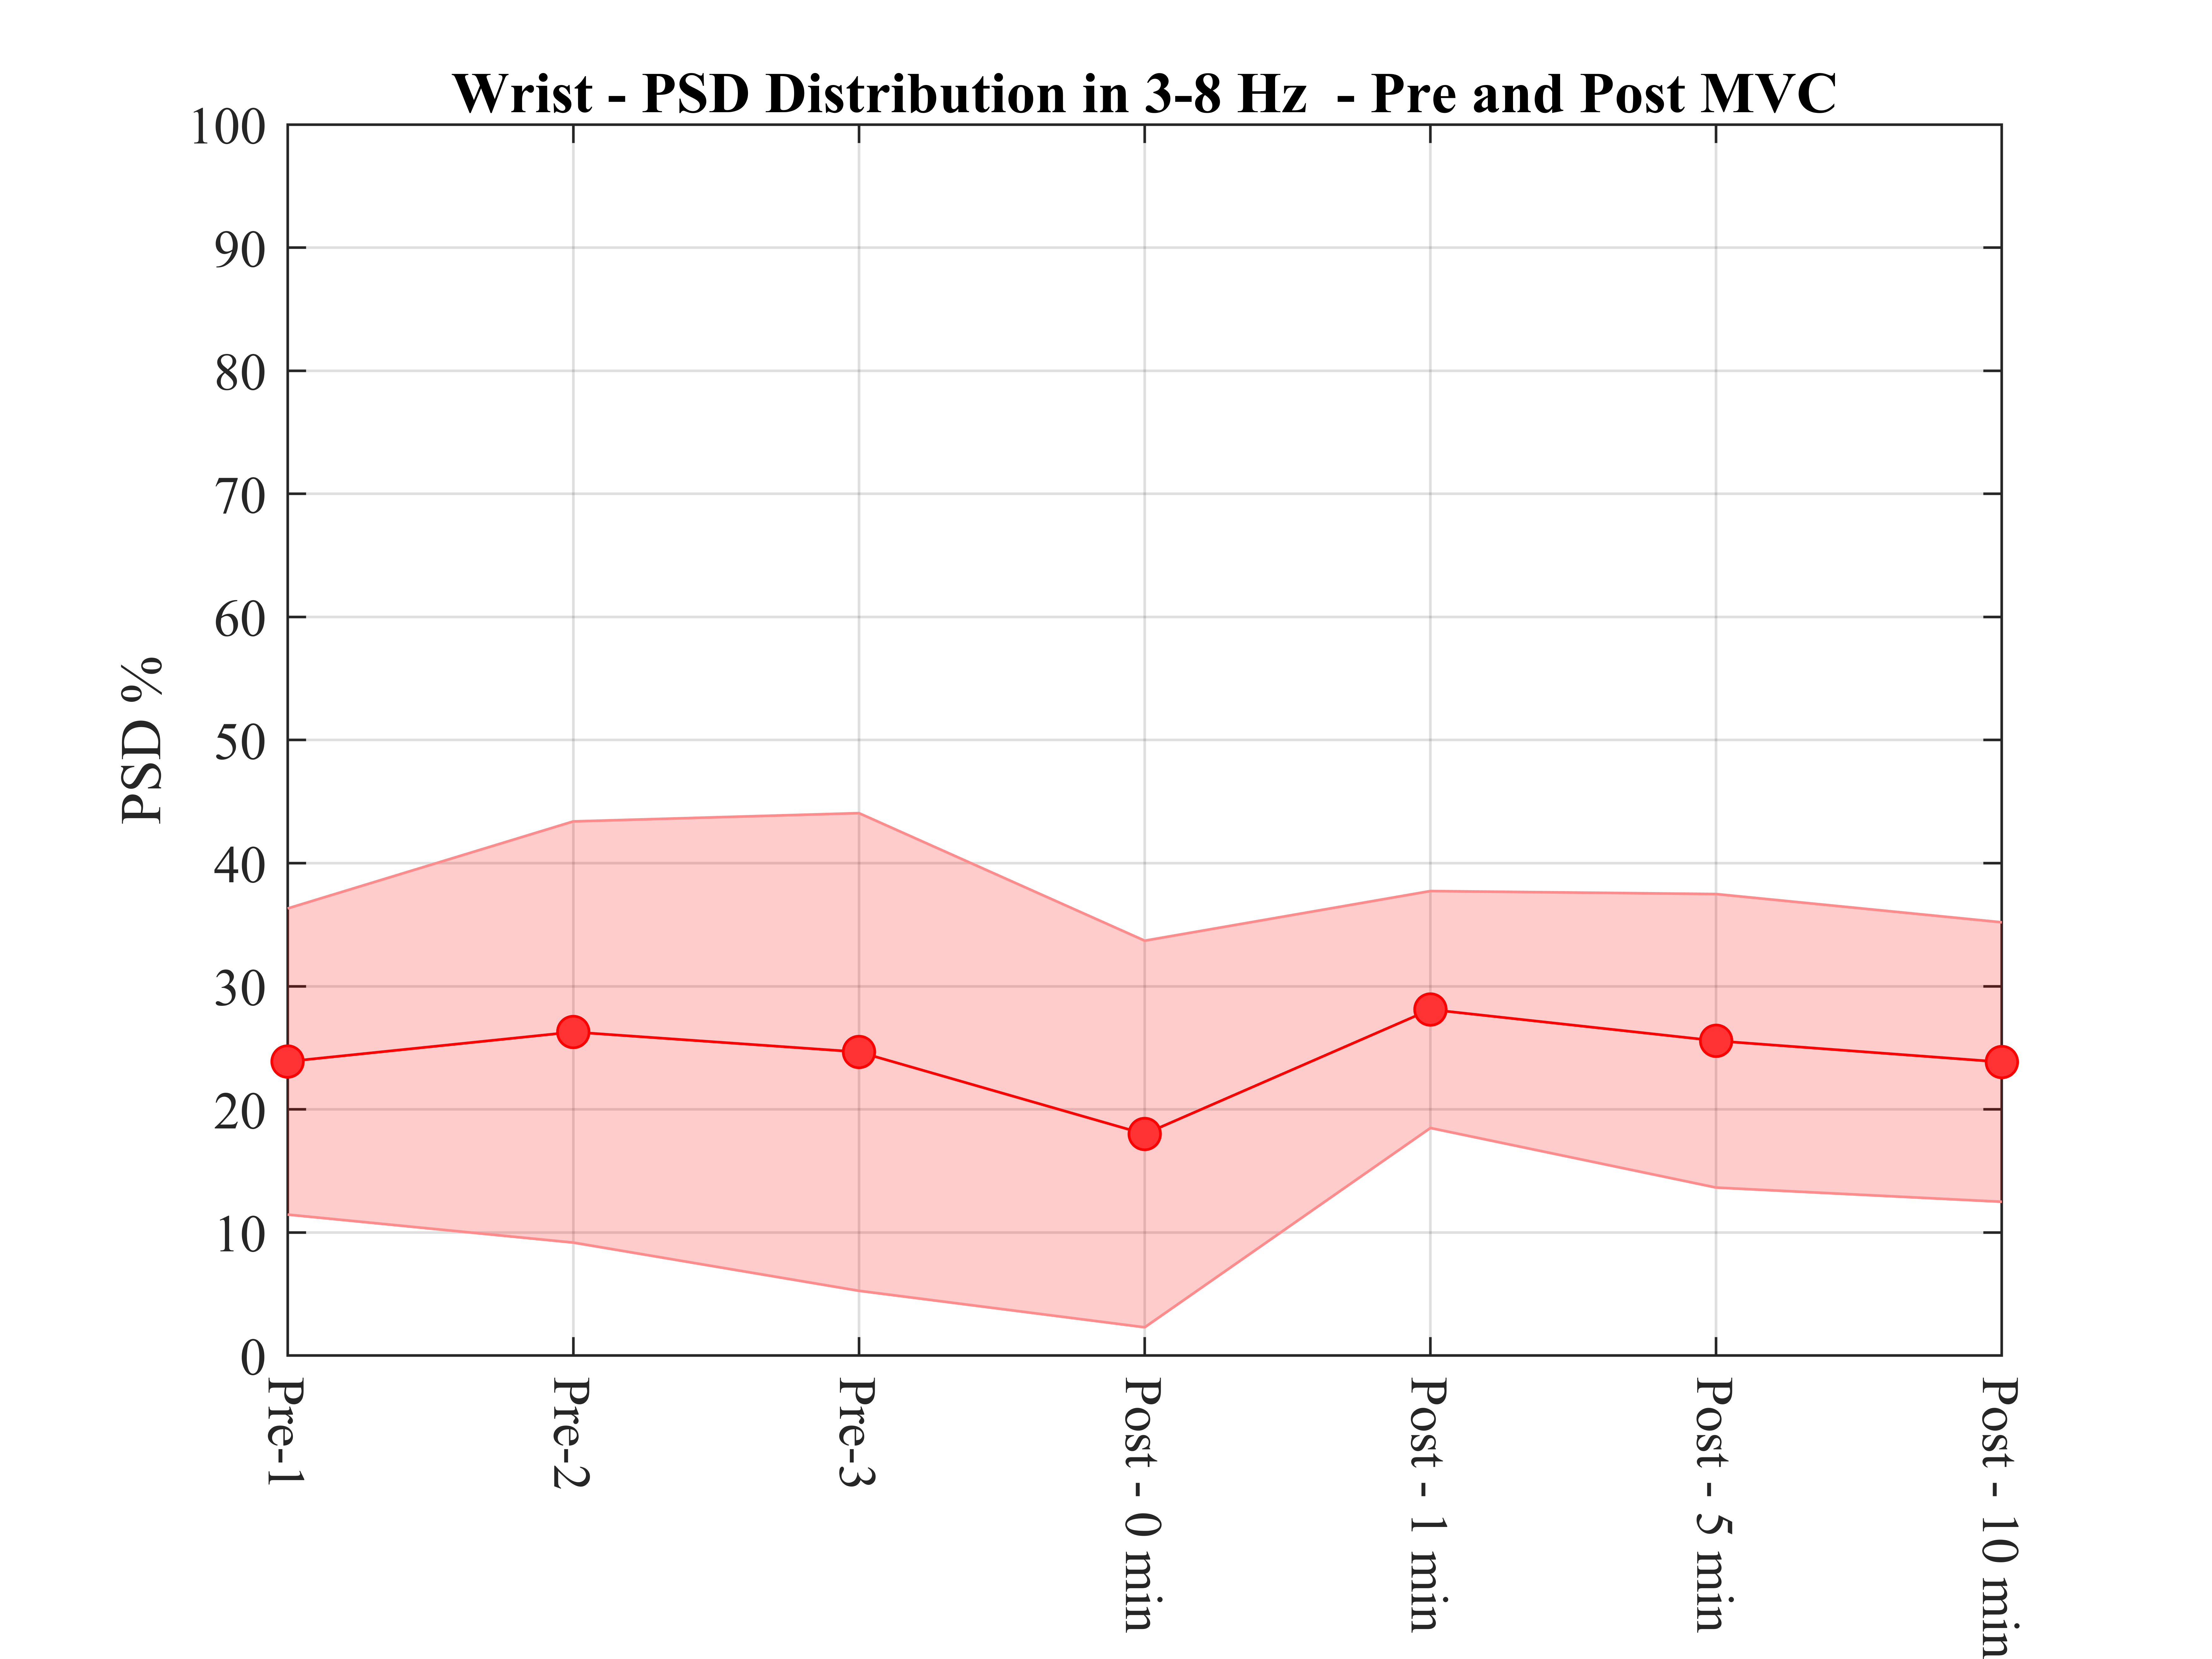
\includegraphics[width=0.31\textwidth]{Figures/wrist_pre_and_postMVC-ept_shaded_3_8.tex}}
	\label{fig:wrist_pre30MVC}
	\hfill
	\subfloat[Wrist: 8 - 14 Hz]{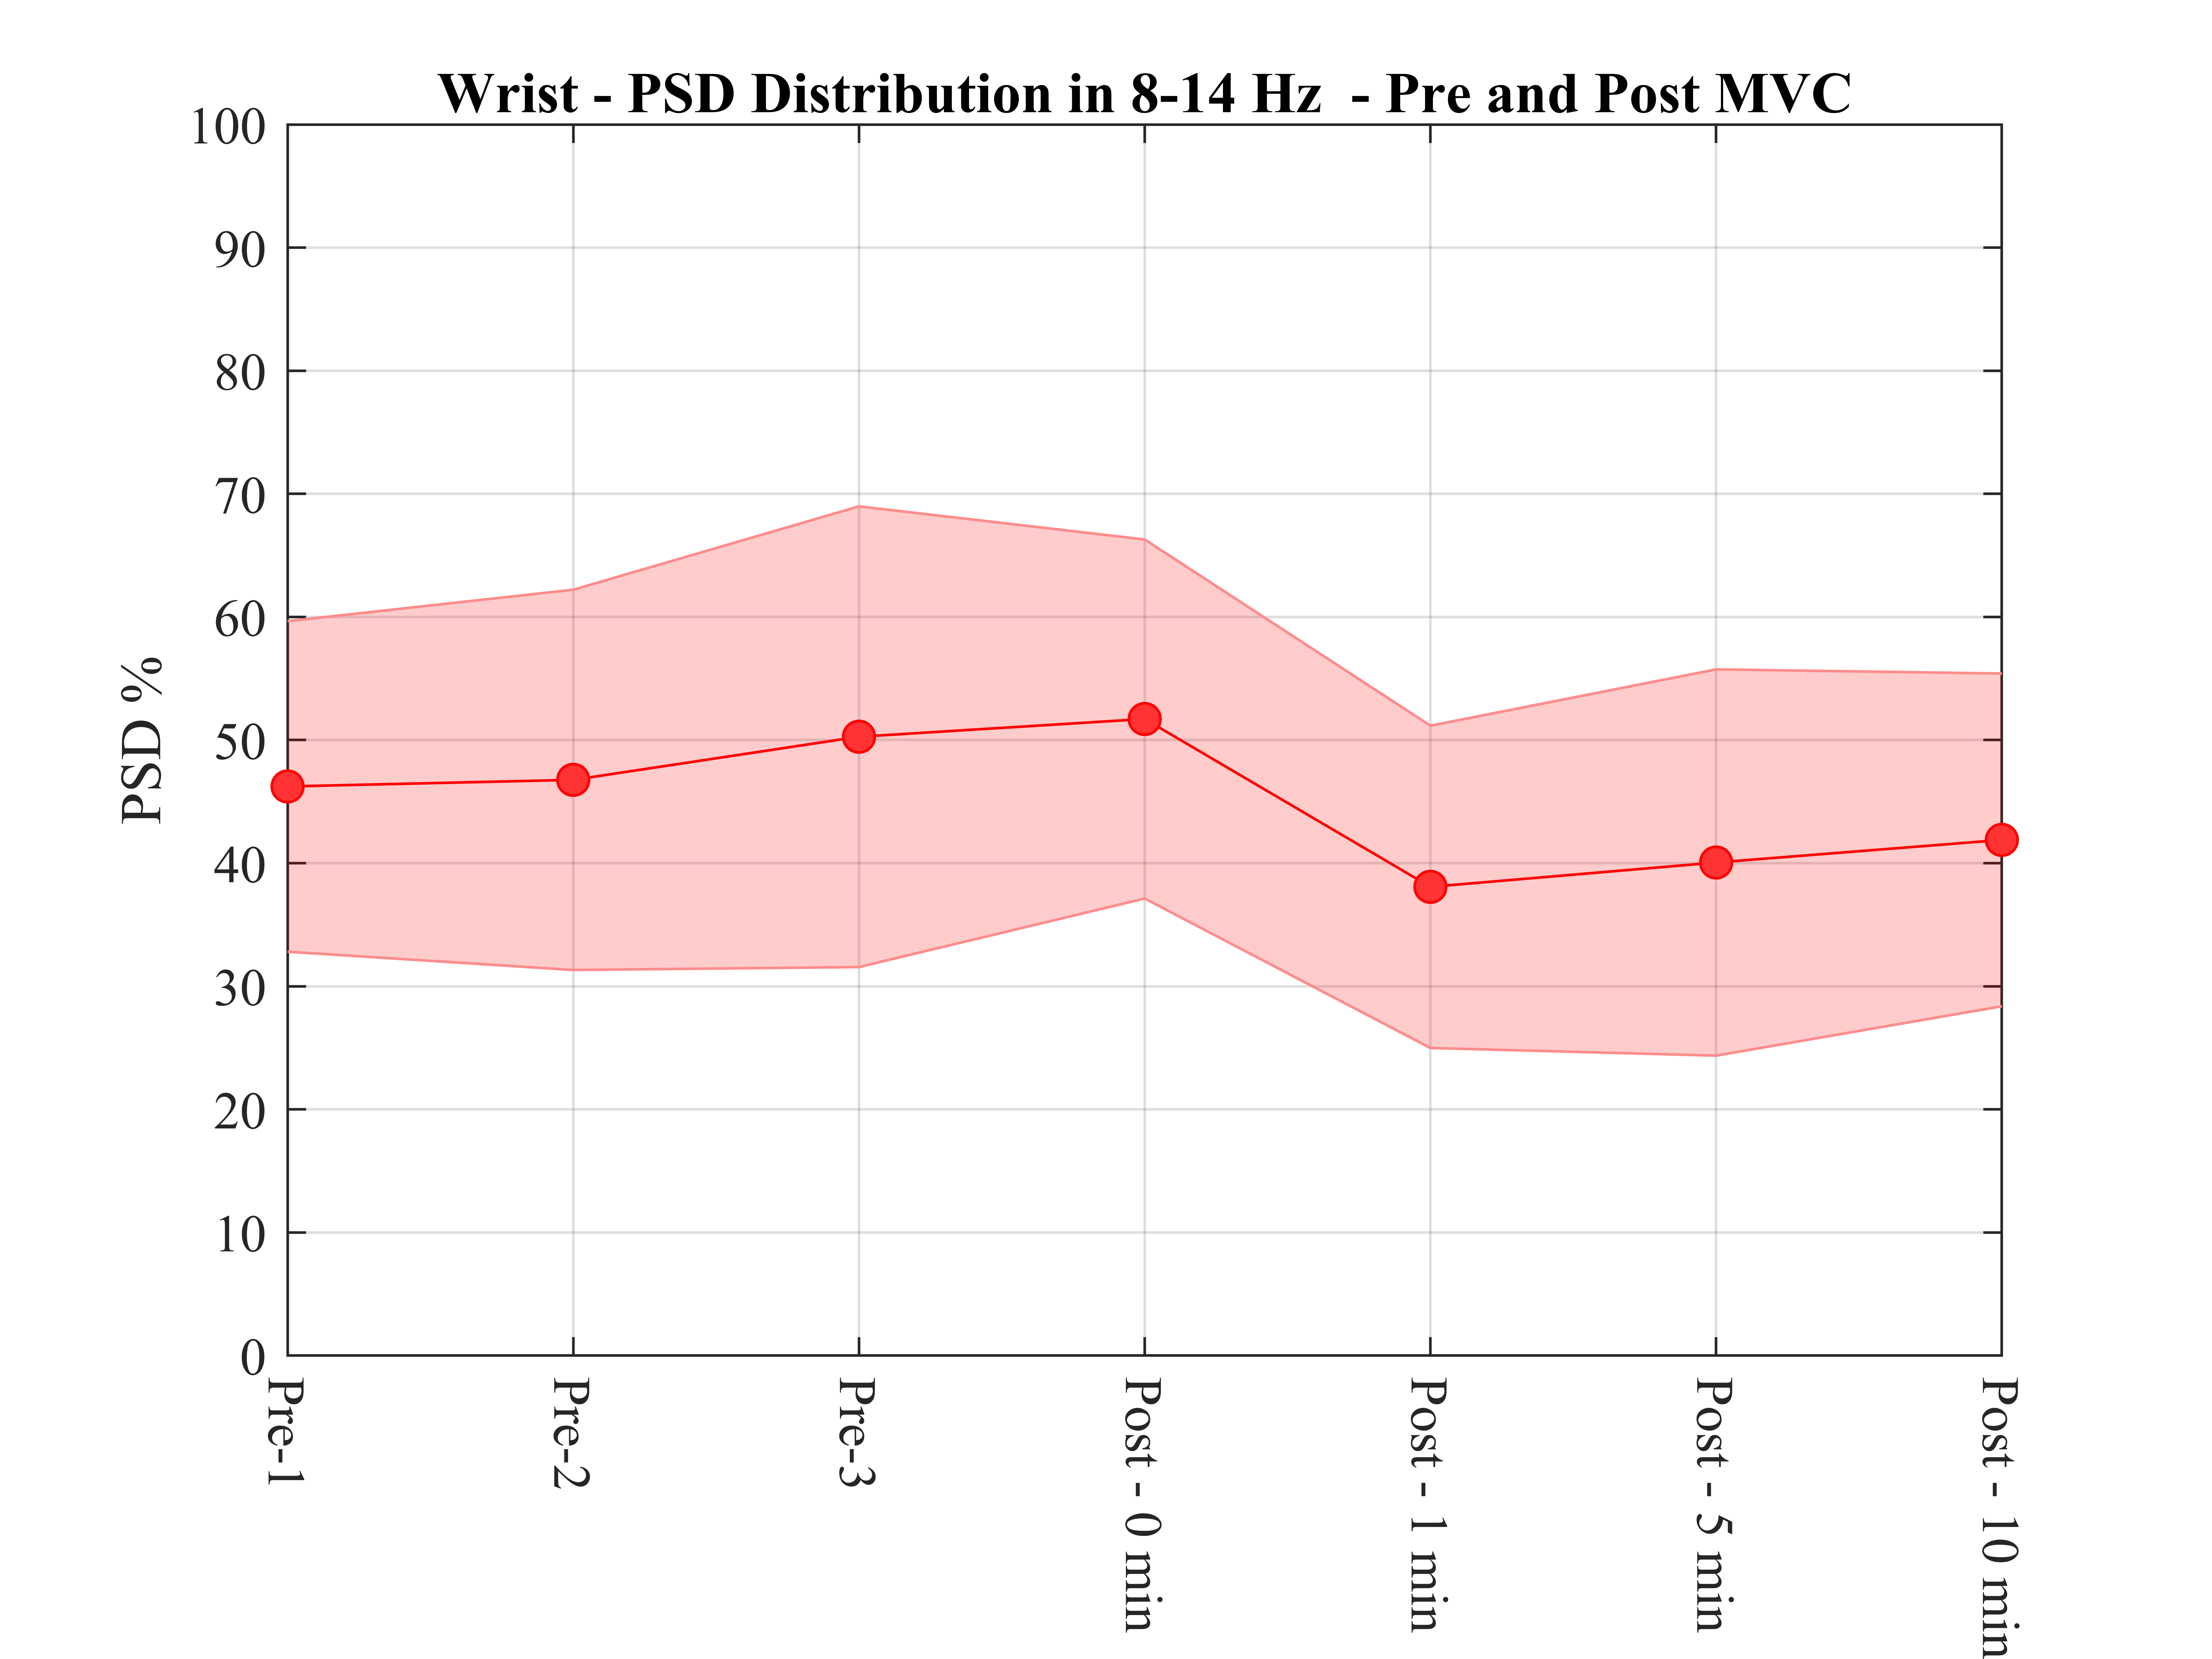
\includegraphics[width=0.31\textwidth]{Figures/wrist_pre_and_postMVC-ept_shaded_8_14.tex}}
	\label{fig:wrist_pre30MVC}
	\hfill
	\subfloat[Wrist: 14 - 22 Hz]{\includegraphics[width=0.31\textwidth]{Figures/wrist_pre_and_postMVC-ept_shaded_14_22.tex}}
	\label{fig:wrist_pre30MVC}
	\medskip
		\subfloat[Finger: 3 - 8 Hz]{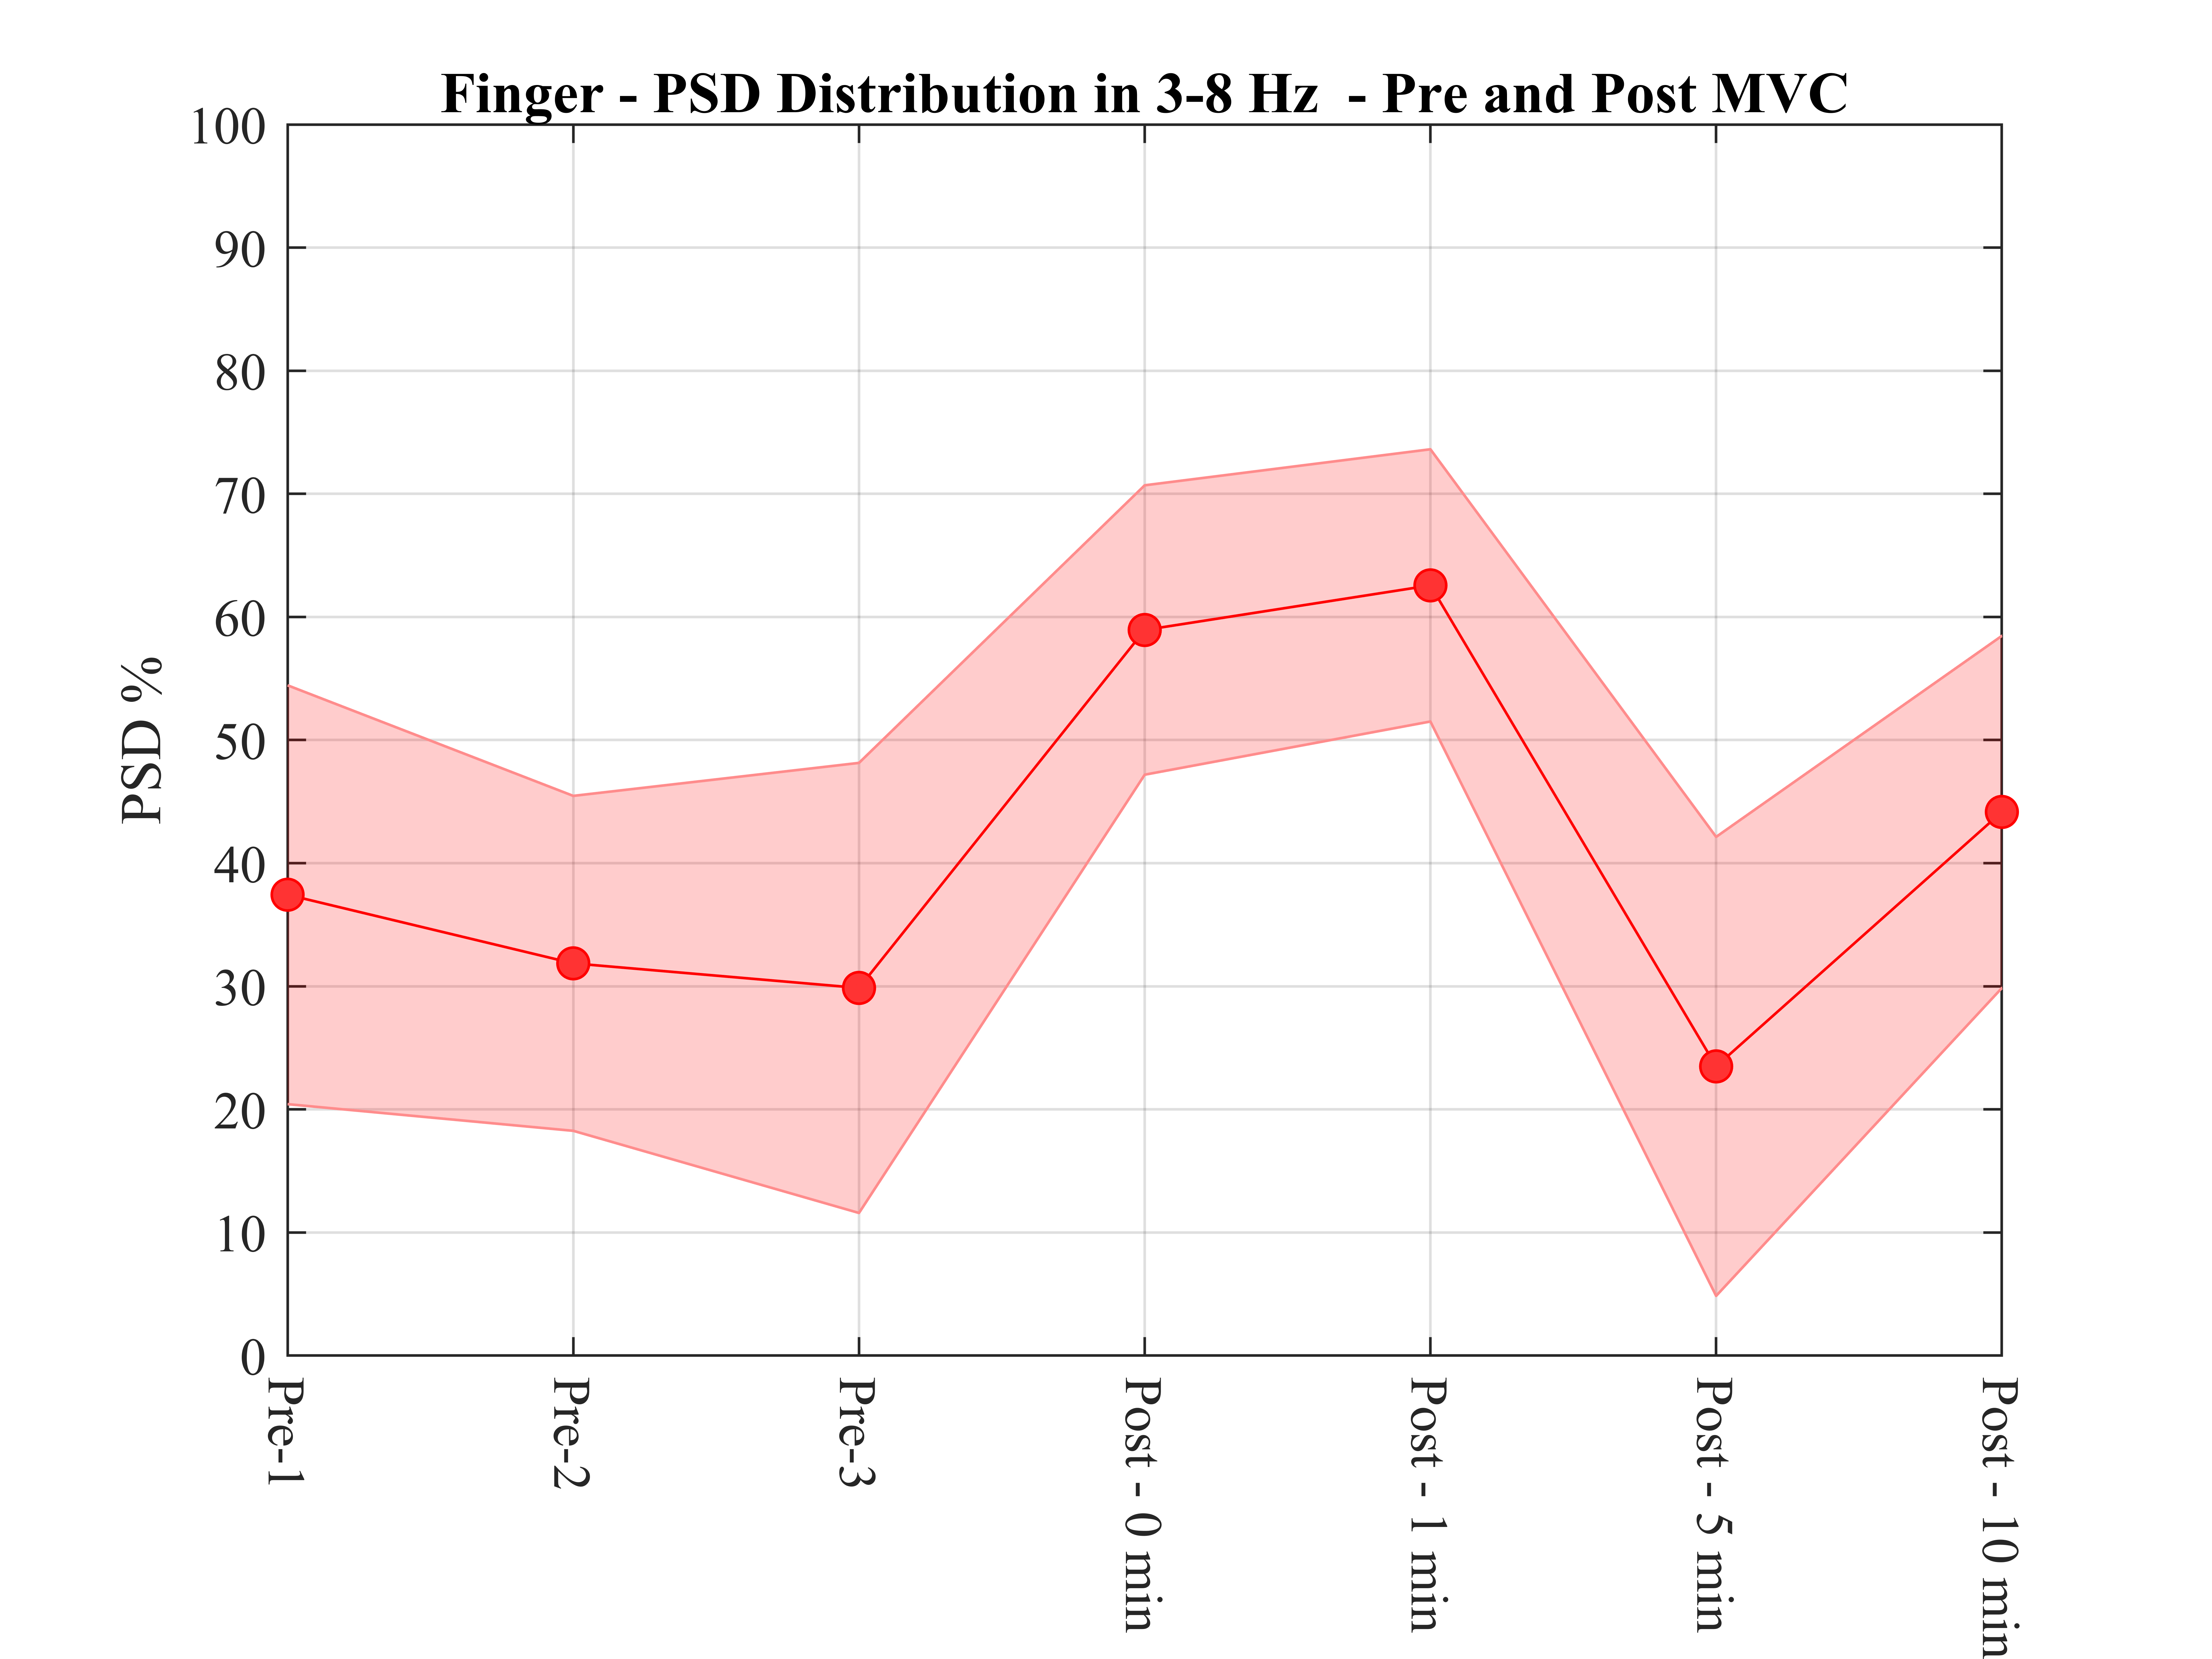
\includegraphics[width=0.31\textwidth]{Figures/finger_pre_and_postMVC-ept_shaded_3_8_fatigued.tex}}
	\label{fig:finger_pre30MVC}
	\hfill
	\subfloat[Finger: 8 - 14 Hz]{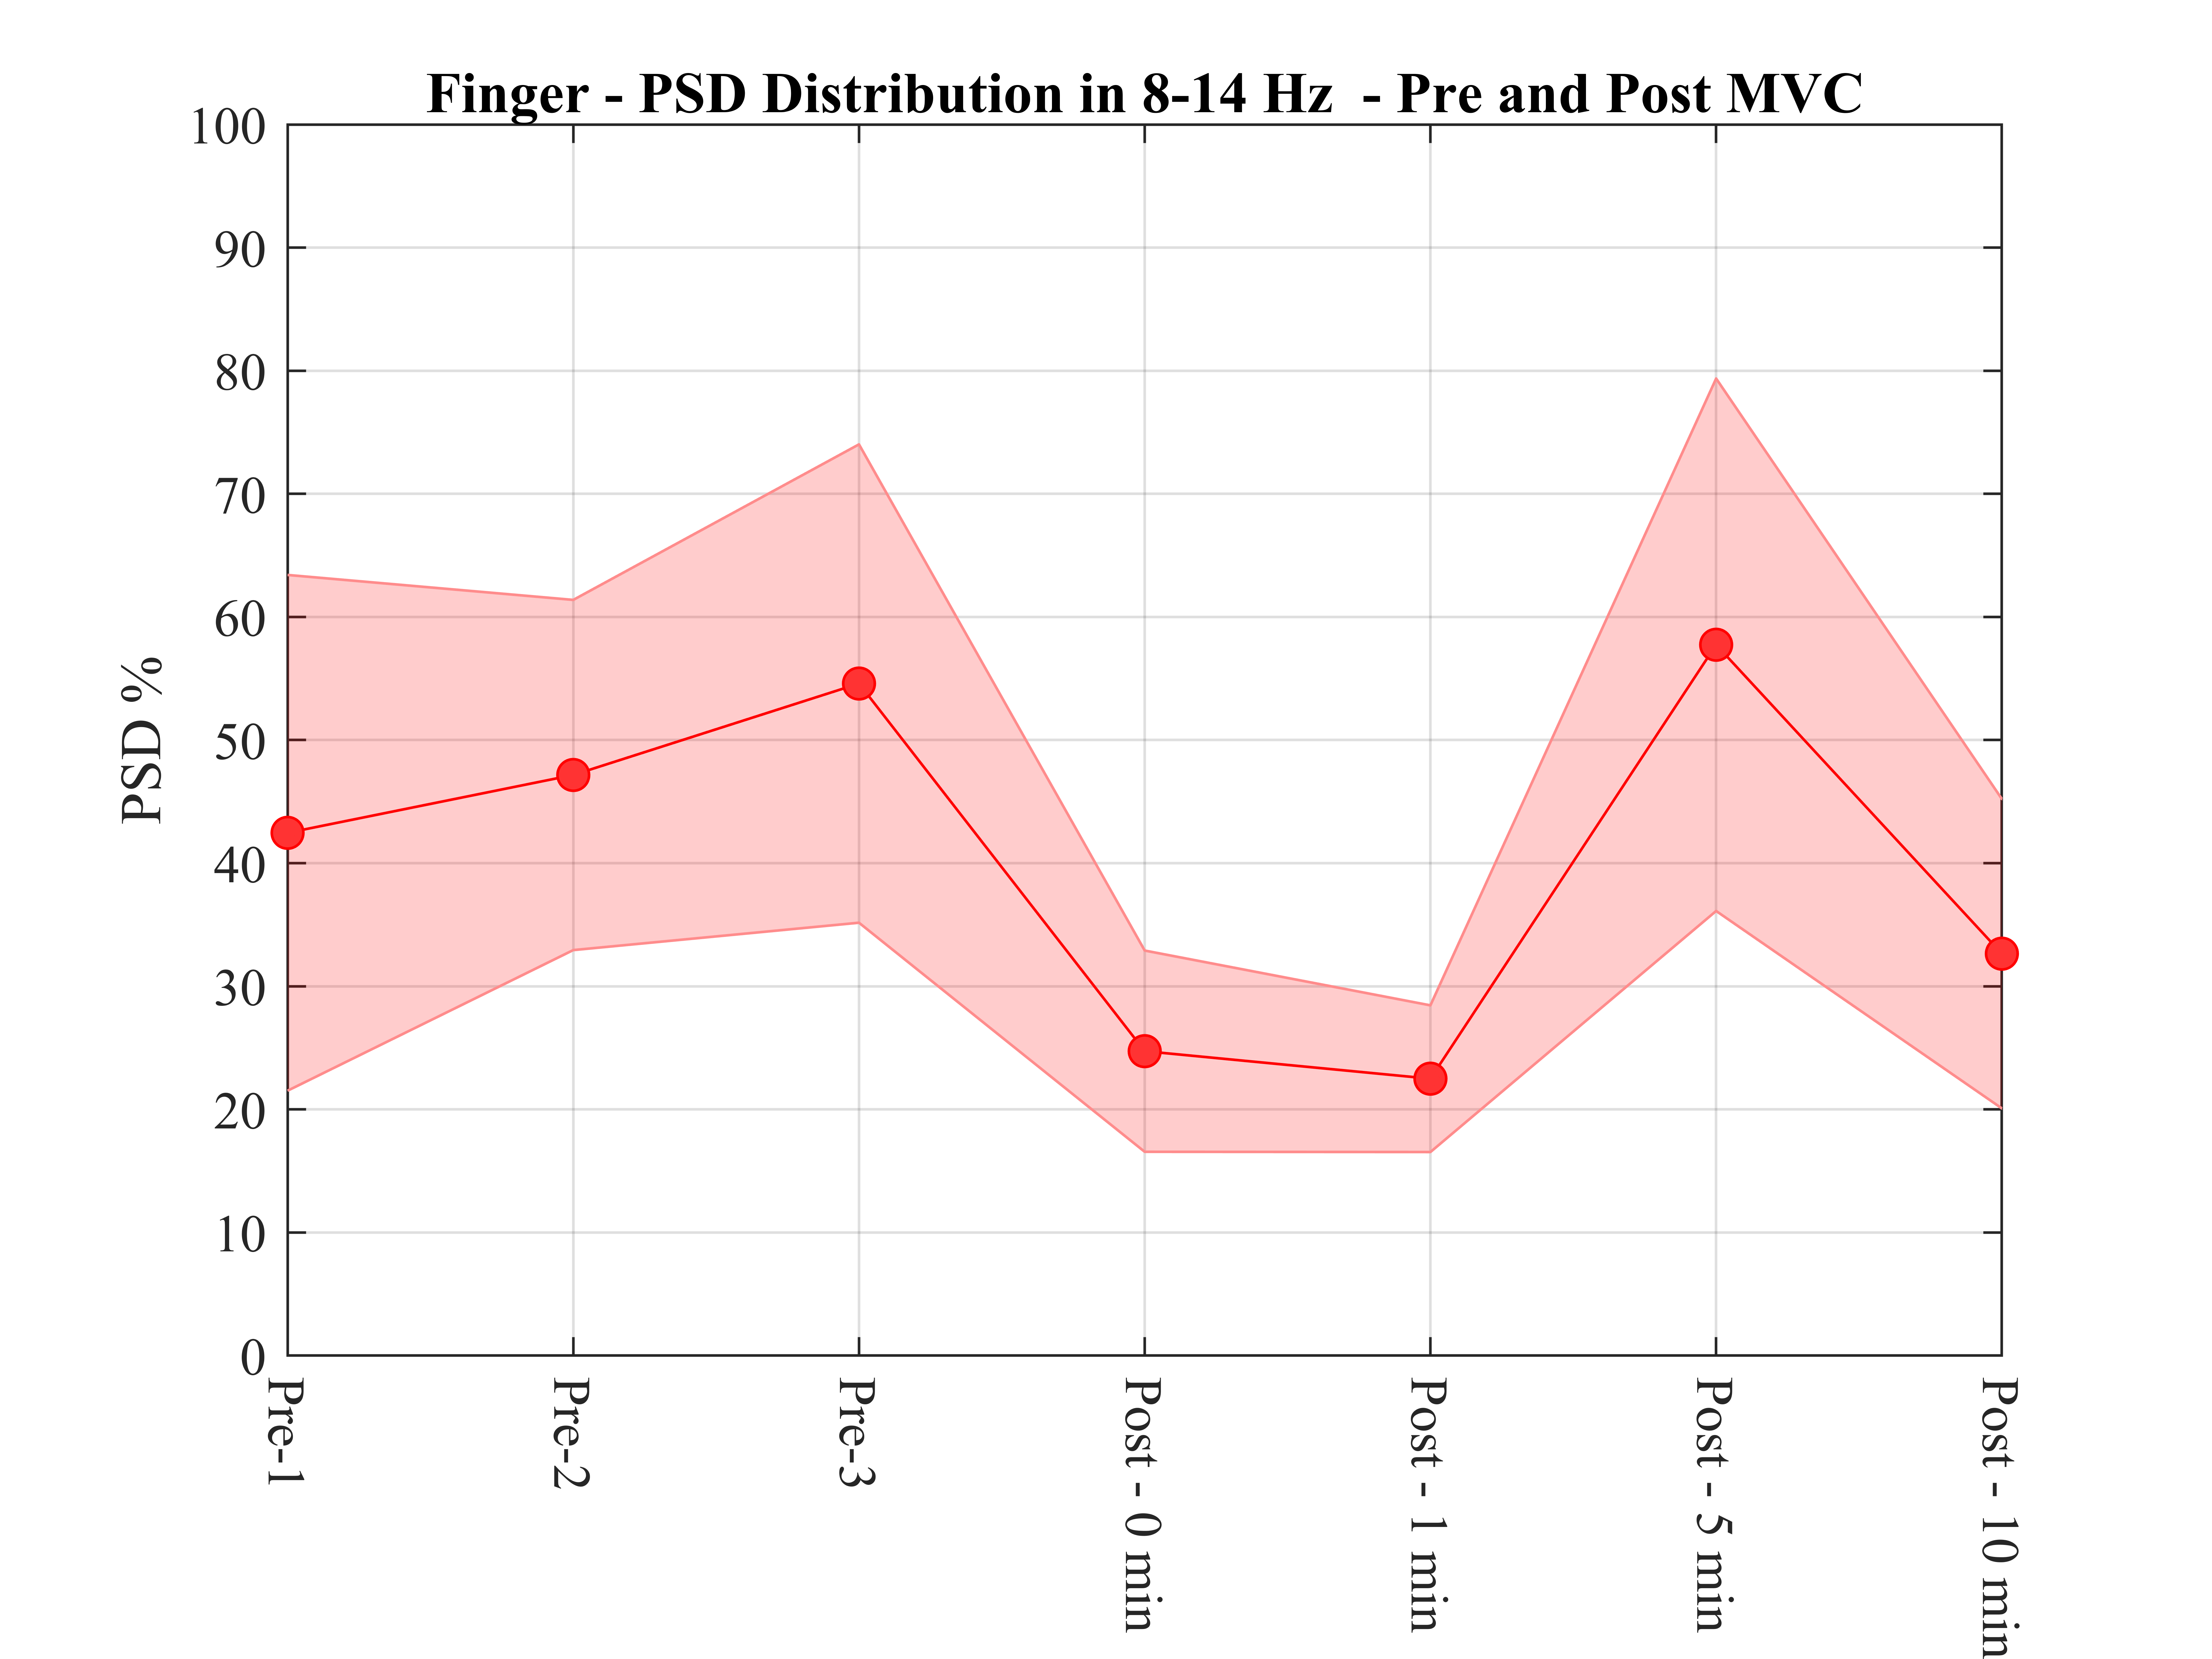
\includegraphics[width=0.31\textwidth]{Figures/finger_pre_and_postMVC-ept_shaded_8_14_fatigued.tex}}
	\label{fig:finger_pre30MVC}
	\hfill
	\subfloat[Finger: 14 - 22 Hz]{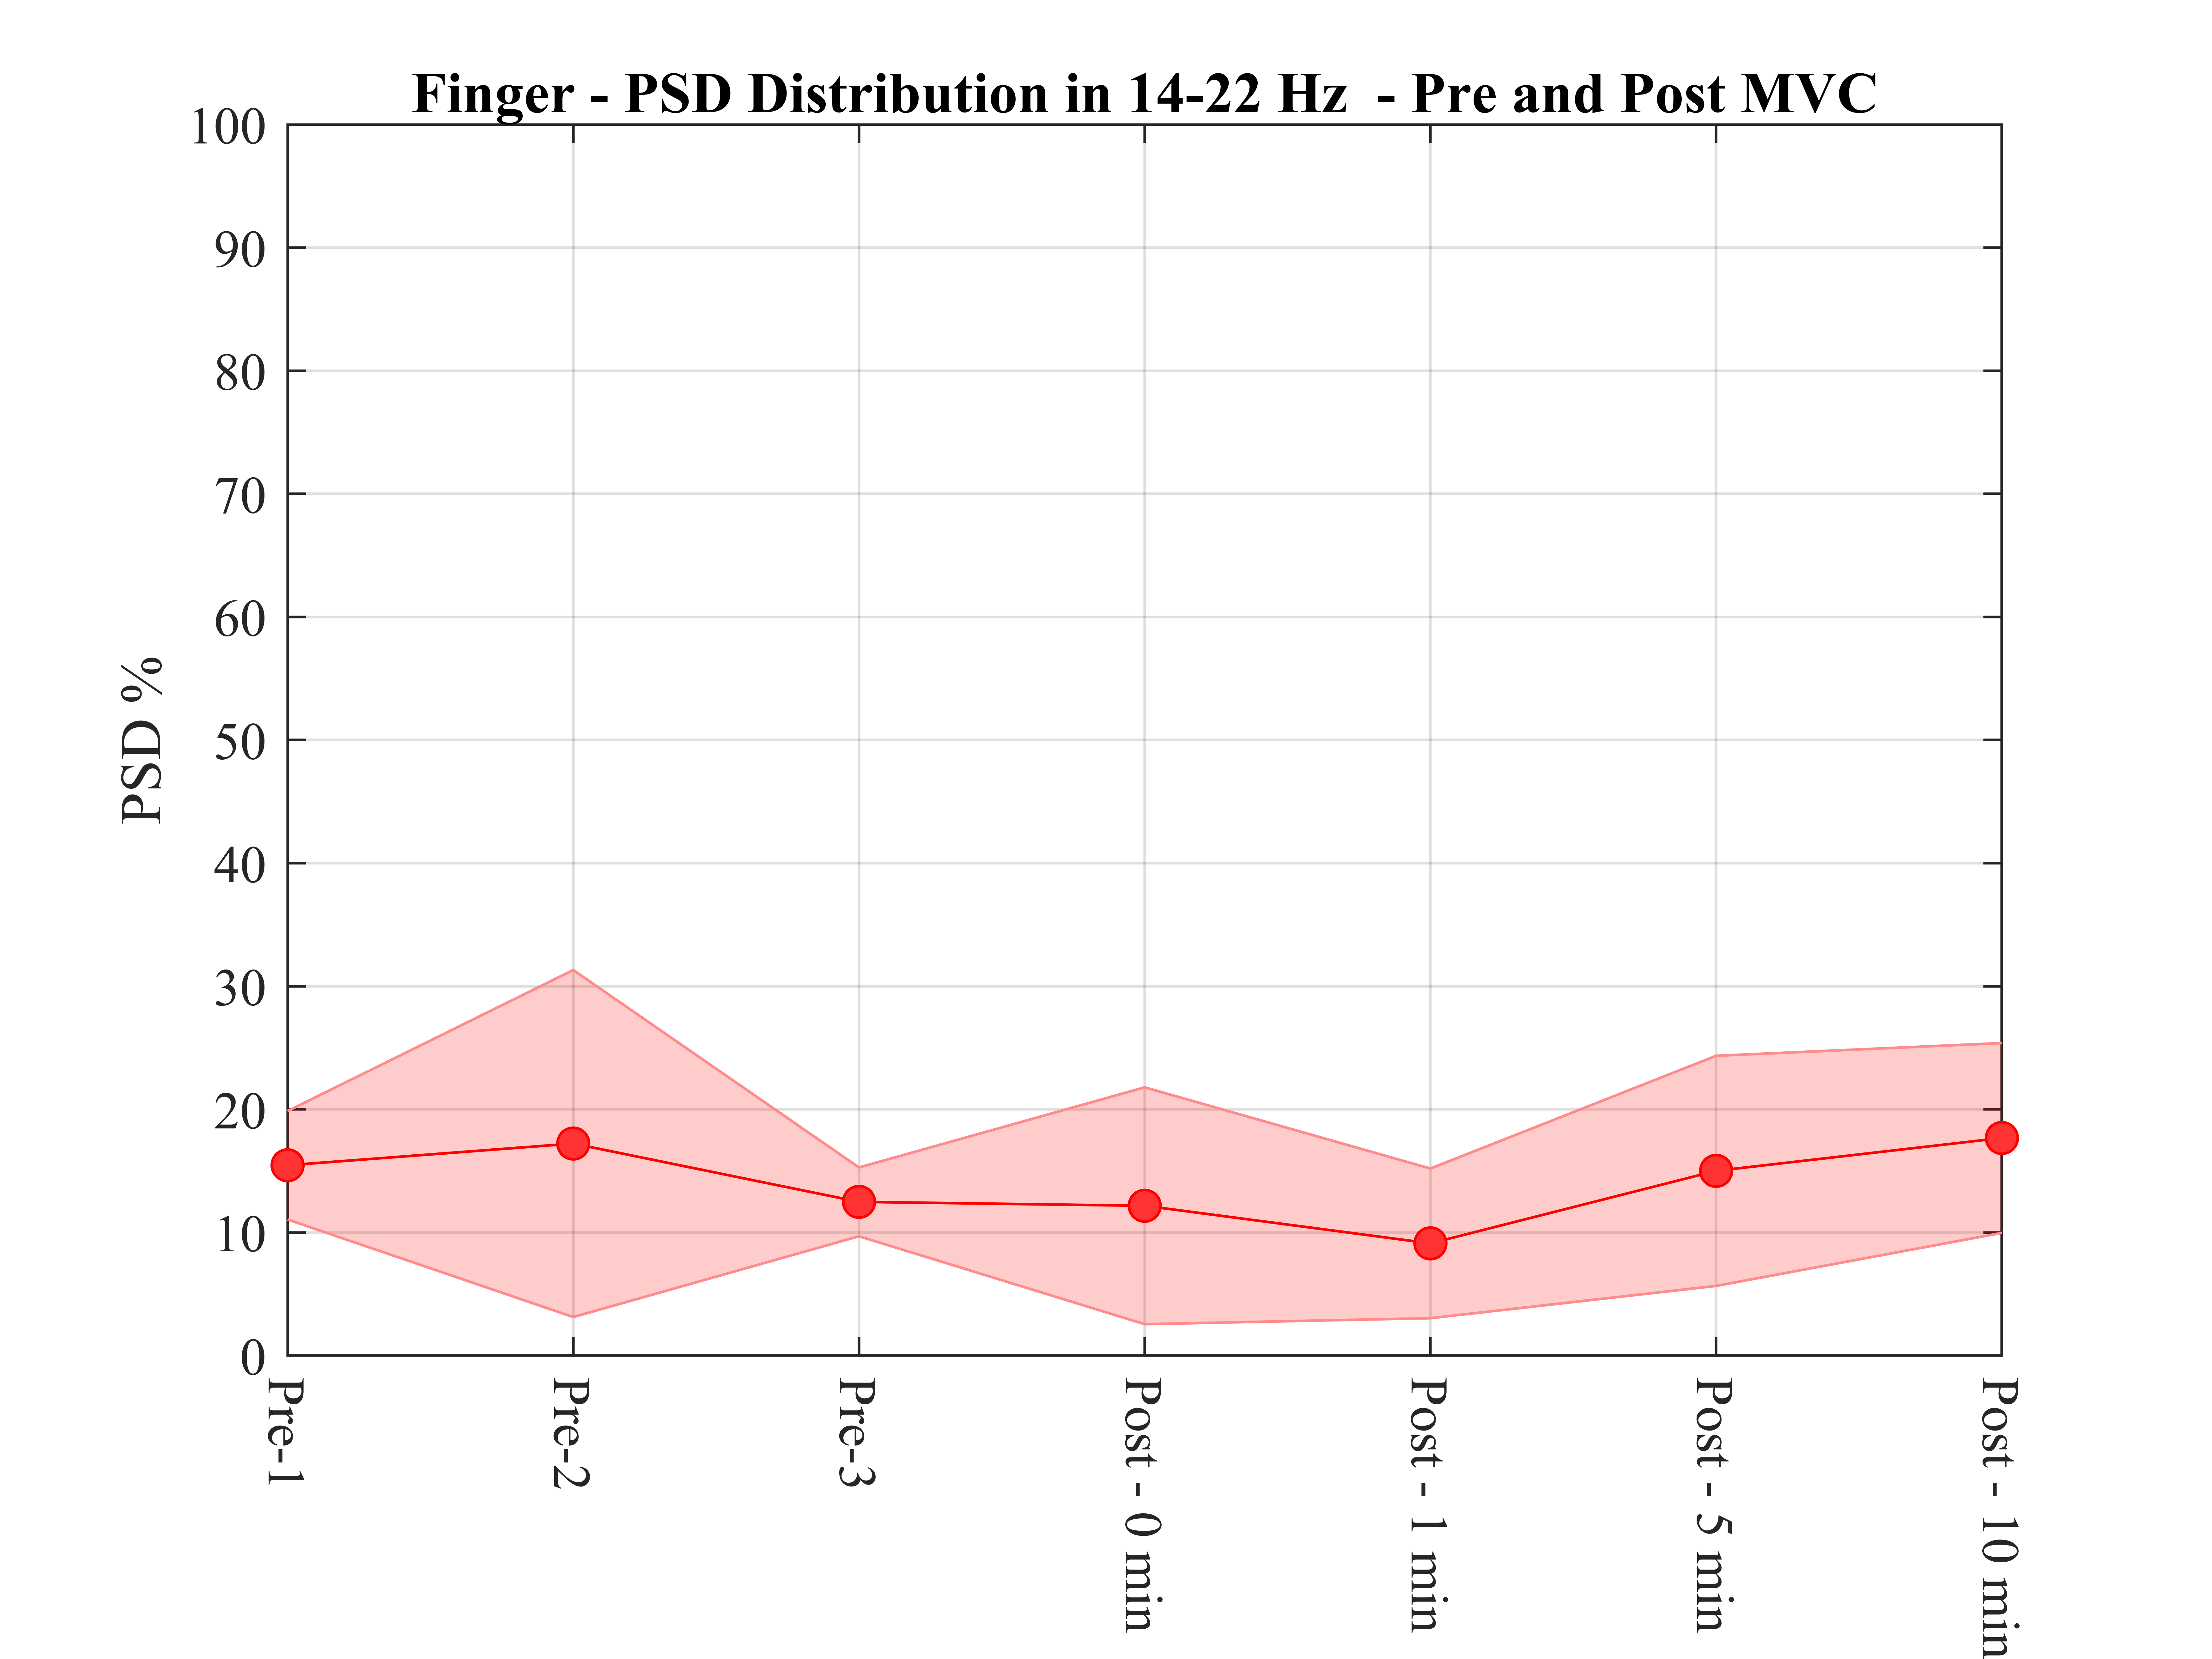
\includegraphics[width=0.31\textwidth]{Figures/finger_pre_and_postMVC-ept_shaded_14_22_fatigued.tex}}
	\label{fig:finger_pre30MVC}
	\caption{Pre and post MVC PSD distribution in different frequency ranges.}
	\label{fig:MVC}
	\medskip
\end{figure*}

In the third stage, post-fatigue test ($\sim 3$ min), a cycle which consists of Post-MVC (5 s), posture, resting and loaded posture condition tests each with duration 15 s without rest between exercises was repeated 4 times. The rest period after each cycle of the tasks was progressively increased from 0 to 2 and 4 min. The tremor was measured 0, 1, 5 and 10 min after exhaustion. In this stage, the participant performed the RPE pre-MVC as well as post-MVC 1, 5 and 10 min after tasks.
%

\subsection{Data Analysis}
The output signals obtained from the accelerometer were sampled at 45 Hz and digitized using a 14-bit analog to digital converter. The signals were then fed to a microcontroller placed on the wristband and then transmitted to a computer using a serial cable. All signals were processed using Matlab (release 2018b; The MathWorks, Natick, MA). The acceleration data was synchronized with EMG event markers and split into episodes ($\sim 65$ episodes per person) according to event markers. Each episode data was then passed through a high-pass filter to remove static content. Fast Fourier transforms (FFTs), and power spectral densities (PSDs) were then calculated for the acceleration data.
%

\section{Results and Discussion}
%
\subsection{Pre-fatigue}
%
For pre-fatigue conditions, the amplitude of the tremor in terms of root mean square (RMS) value and its variance at the finger are greater than at the wrist (Fig. \ref{fig:RMS}).

The frequency analysis revealed the tremor with higher frequencies of the finger compared with the wrist in rest, posture and loaded posture condition. The PSD distribution analyses in the 3-8, 8-14, and 14-22 Hz intervals show that most of the peaks are in the first frequency range, especially for the finger tremor (Table \ref{tab:features}). In the case of rest condition, the variance of the PSD distribution on finger tremor is bigger than on the wrist in all three frequency ranges. When the participants do posture and loaded posture condition, the variance of the wrist is almost equal or bigger than of the fingers, which could be explained with their physical status and ability to do simple exercises without fatigue. During the test, personal fatigue is estimated by participants using the RPE scale.

For the rest, posture and loaded posture conditions, the tremor can be detected better on the finger as around 50\% of the tremors are in 3-8 Hz range.
% 
\begin{figure*}[!t]
	\centering
	\subfloat[Wrist: 3 - 8 Hz]{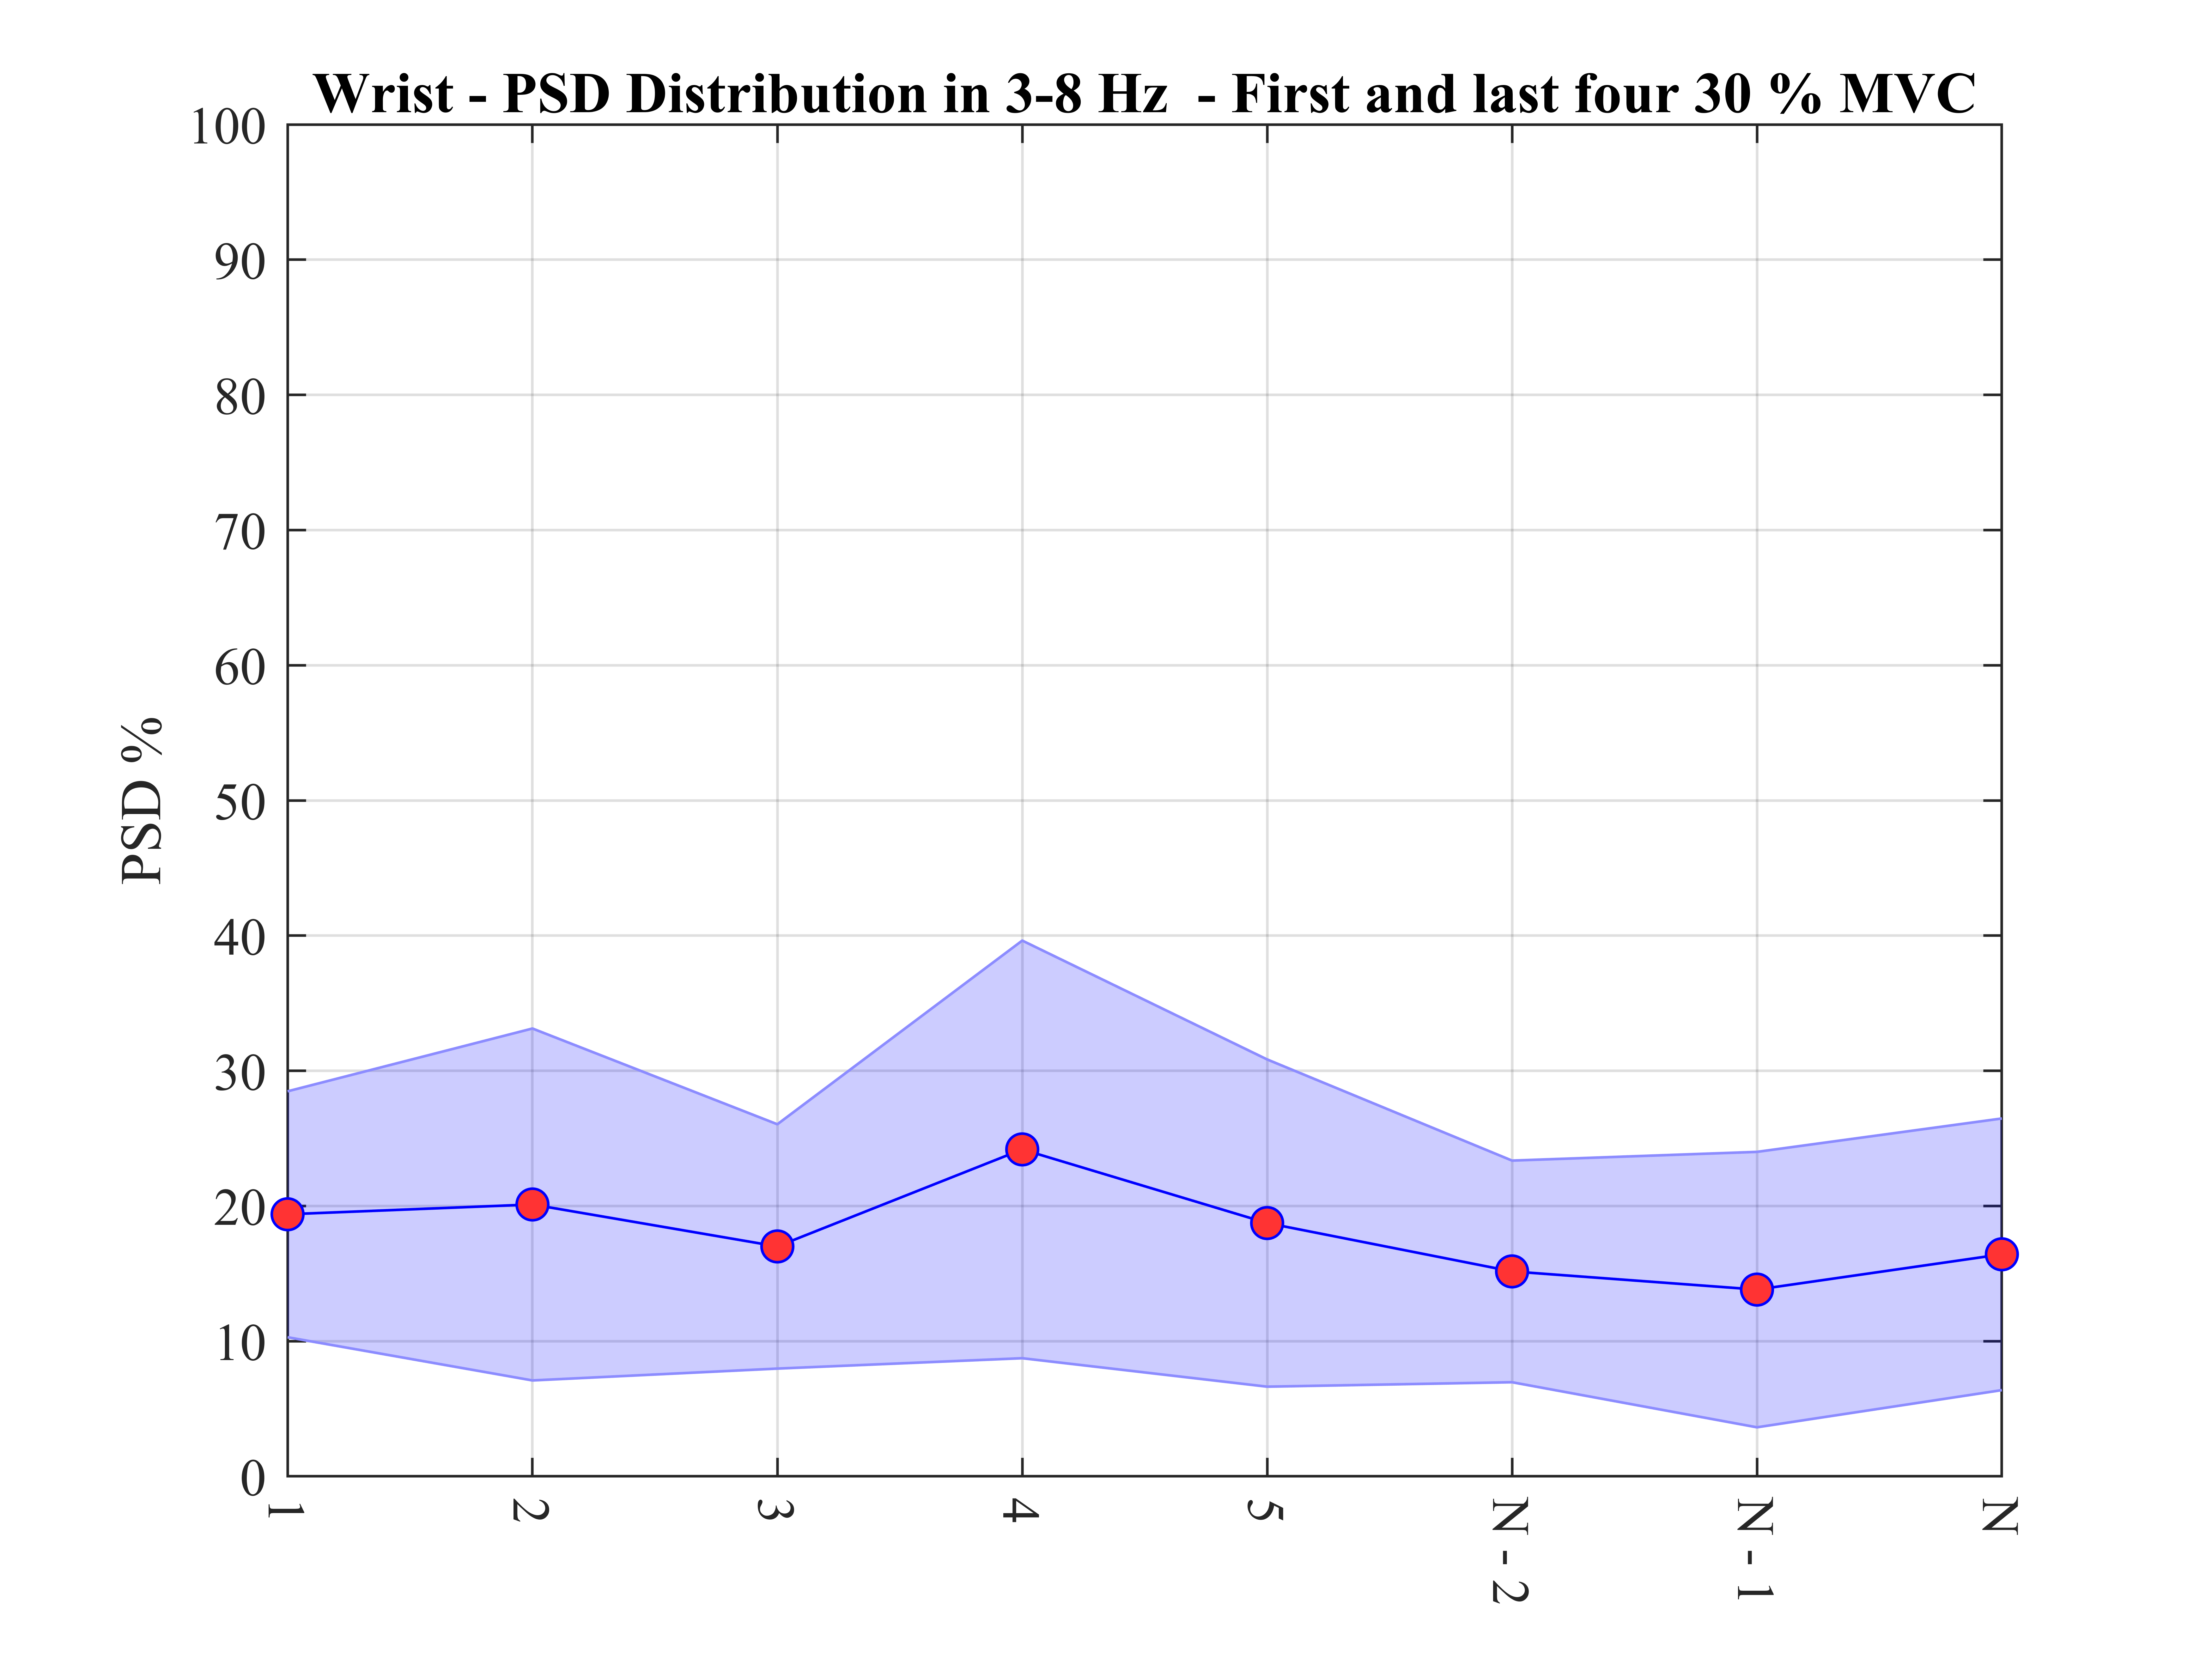
\includegraphics[width=0.31\textwidth]{Figures/wrist_first_and_last_30_MVC-ept_shaded_3_8.tex}}
	\label{fig:wrist_first30MVC}
	\hfill
	\subfloat[Wrist: 8 - 14 Hz]{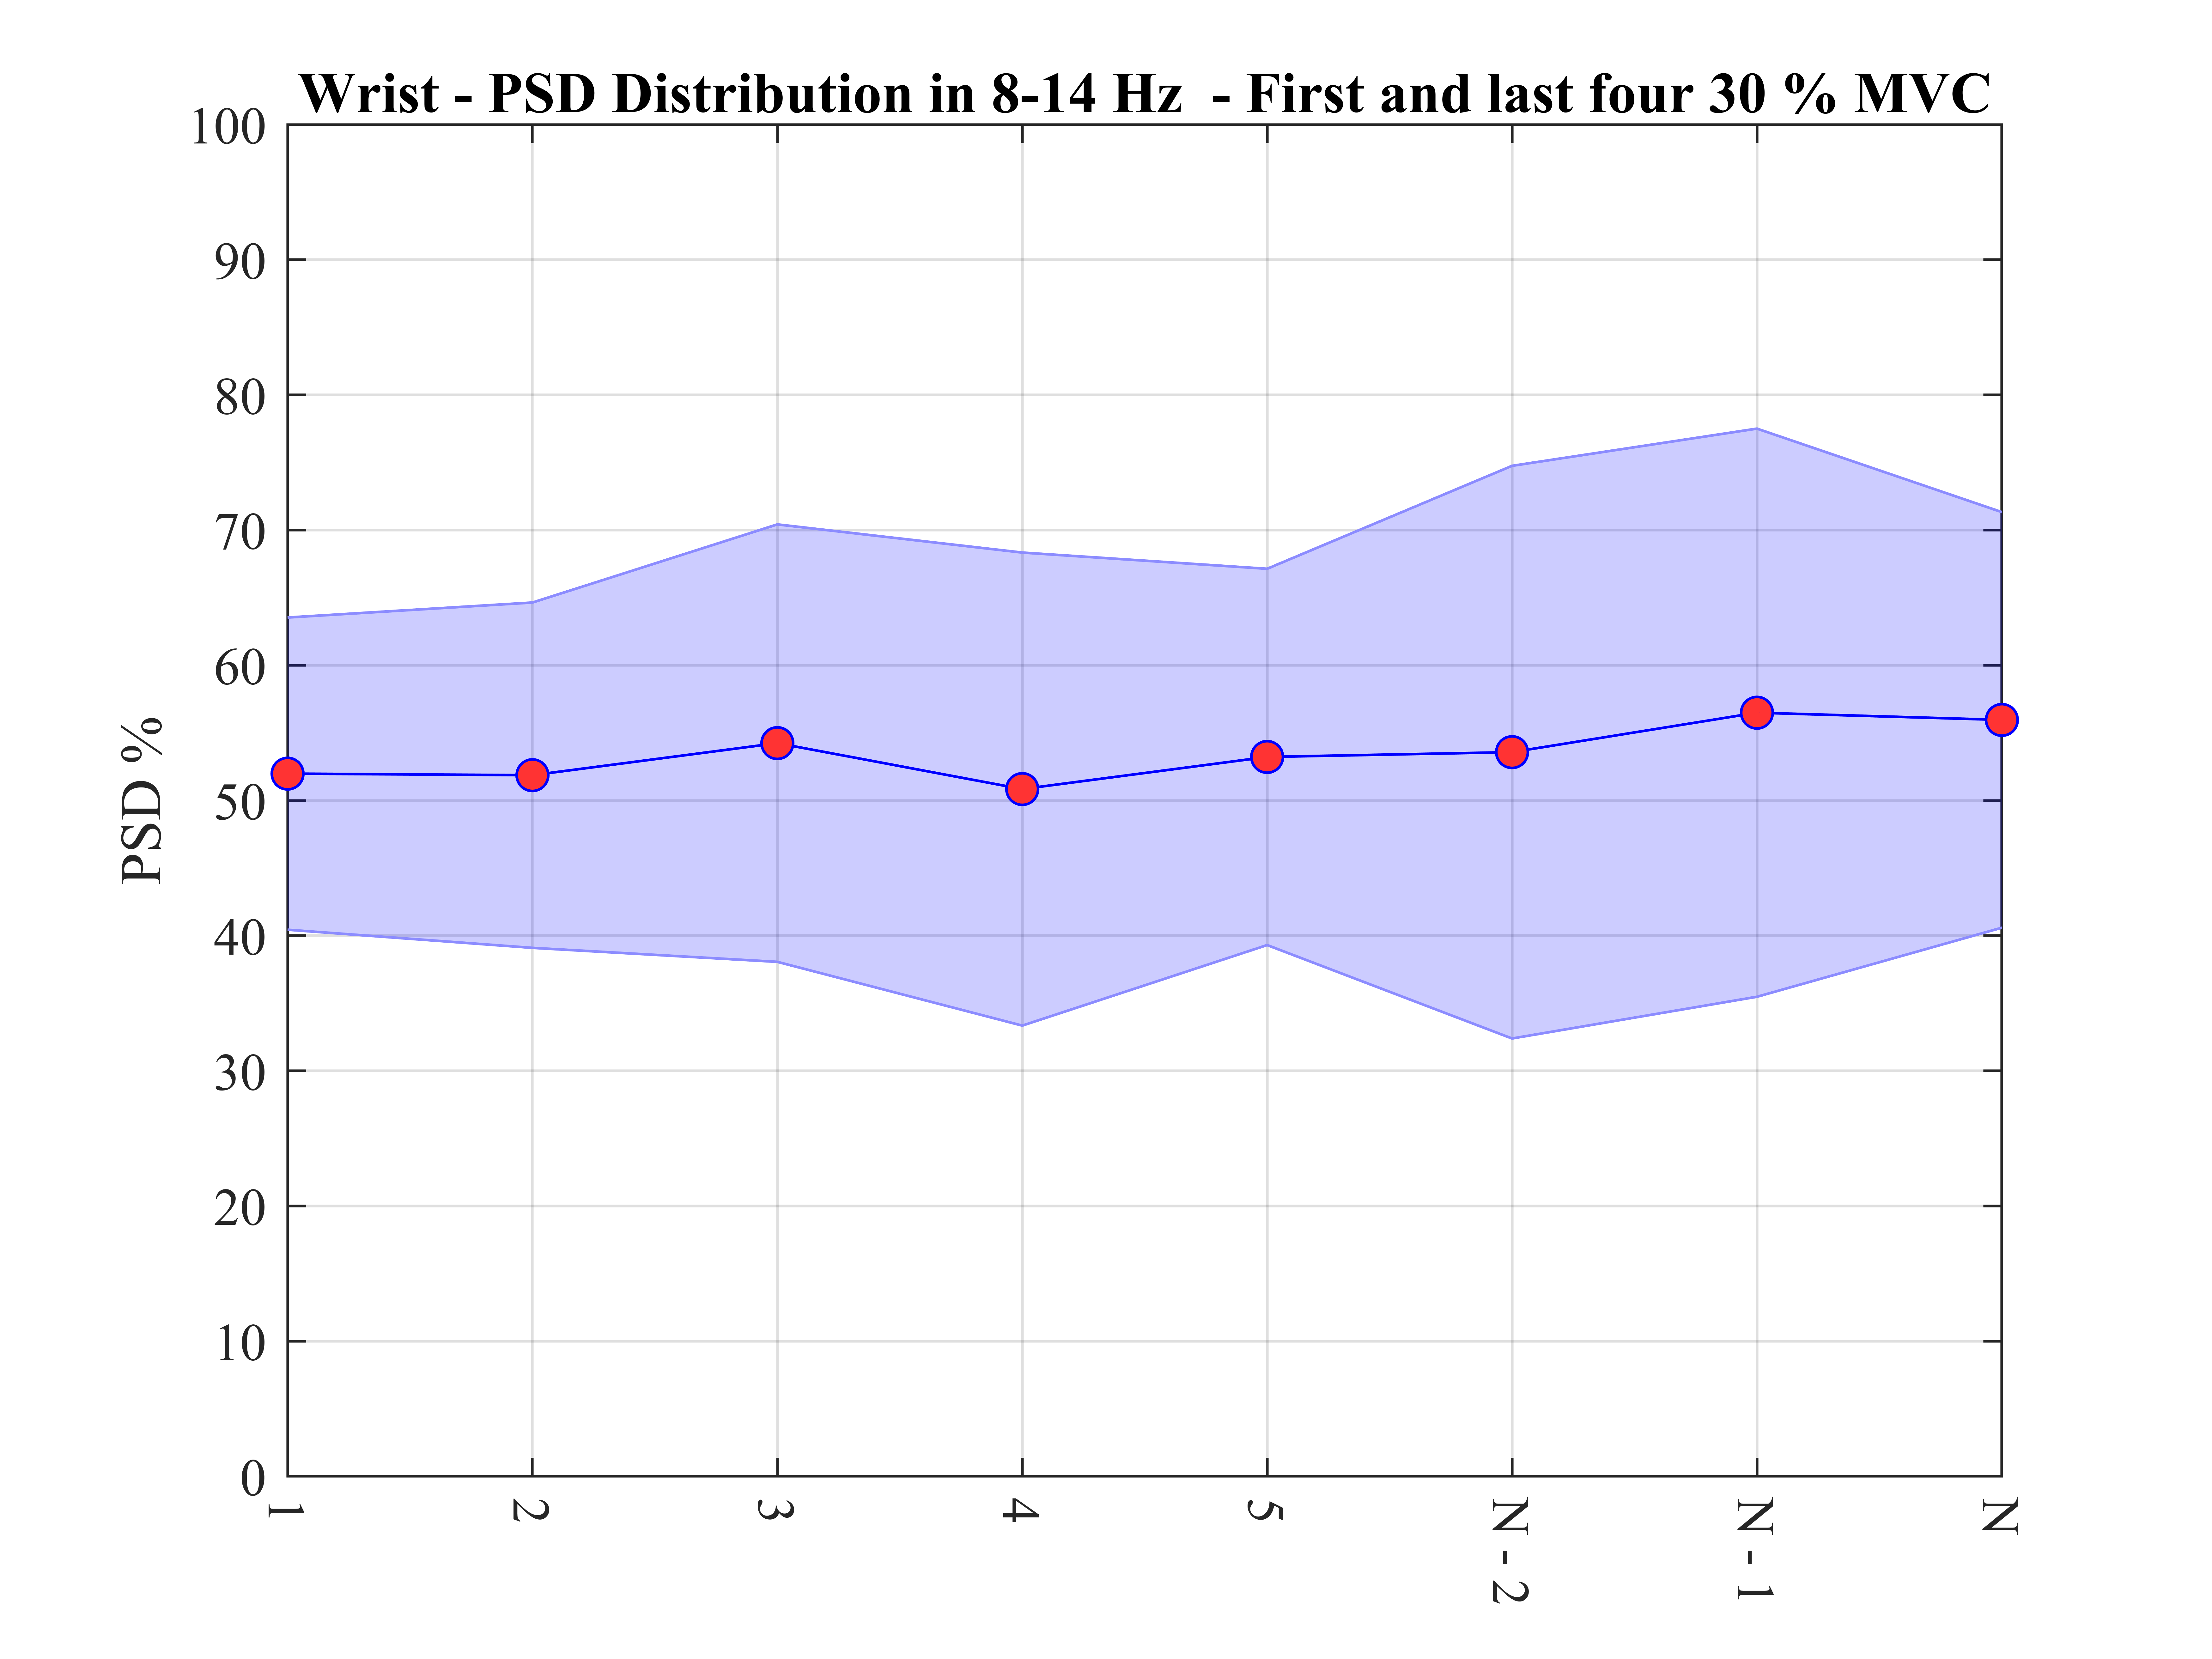
\includegraphics[width=0.31\textwidth]{Figures/wrist_first_and_last_30_MVC-ept_shaded_8_14.tex}}
	\label{fig:wrist_first30MVC}
	\hfill
	\subfloat[Wrist: 14 - 22 Hz]{\includegraphics[width=0.31\textwidth]{Figures/wrist_first_and_last_30_MVC-ept_shaded_14_22.tex}}
	\label{fig:wrist_firstMVC}
	\medskip
	\subfloat[Finger: 3 - 8 Hz]{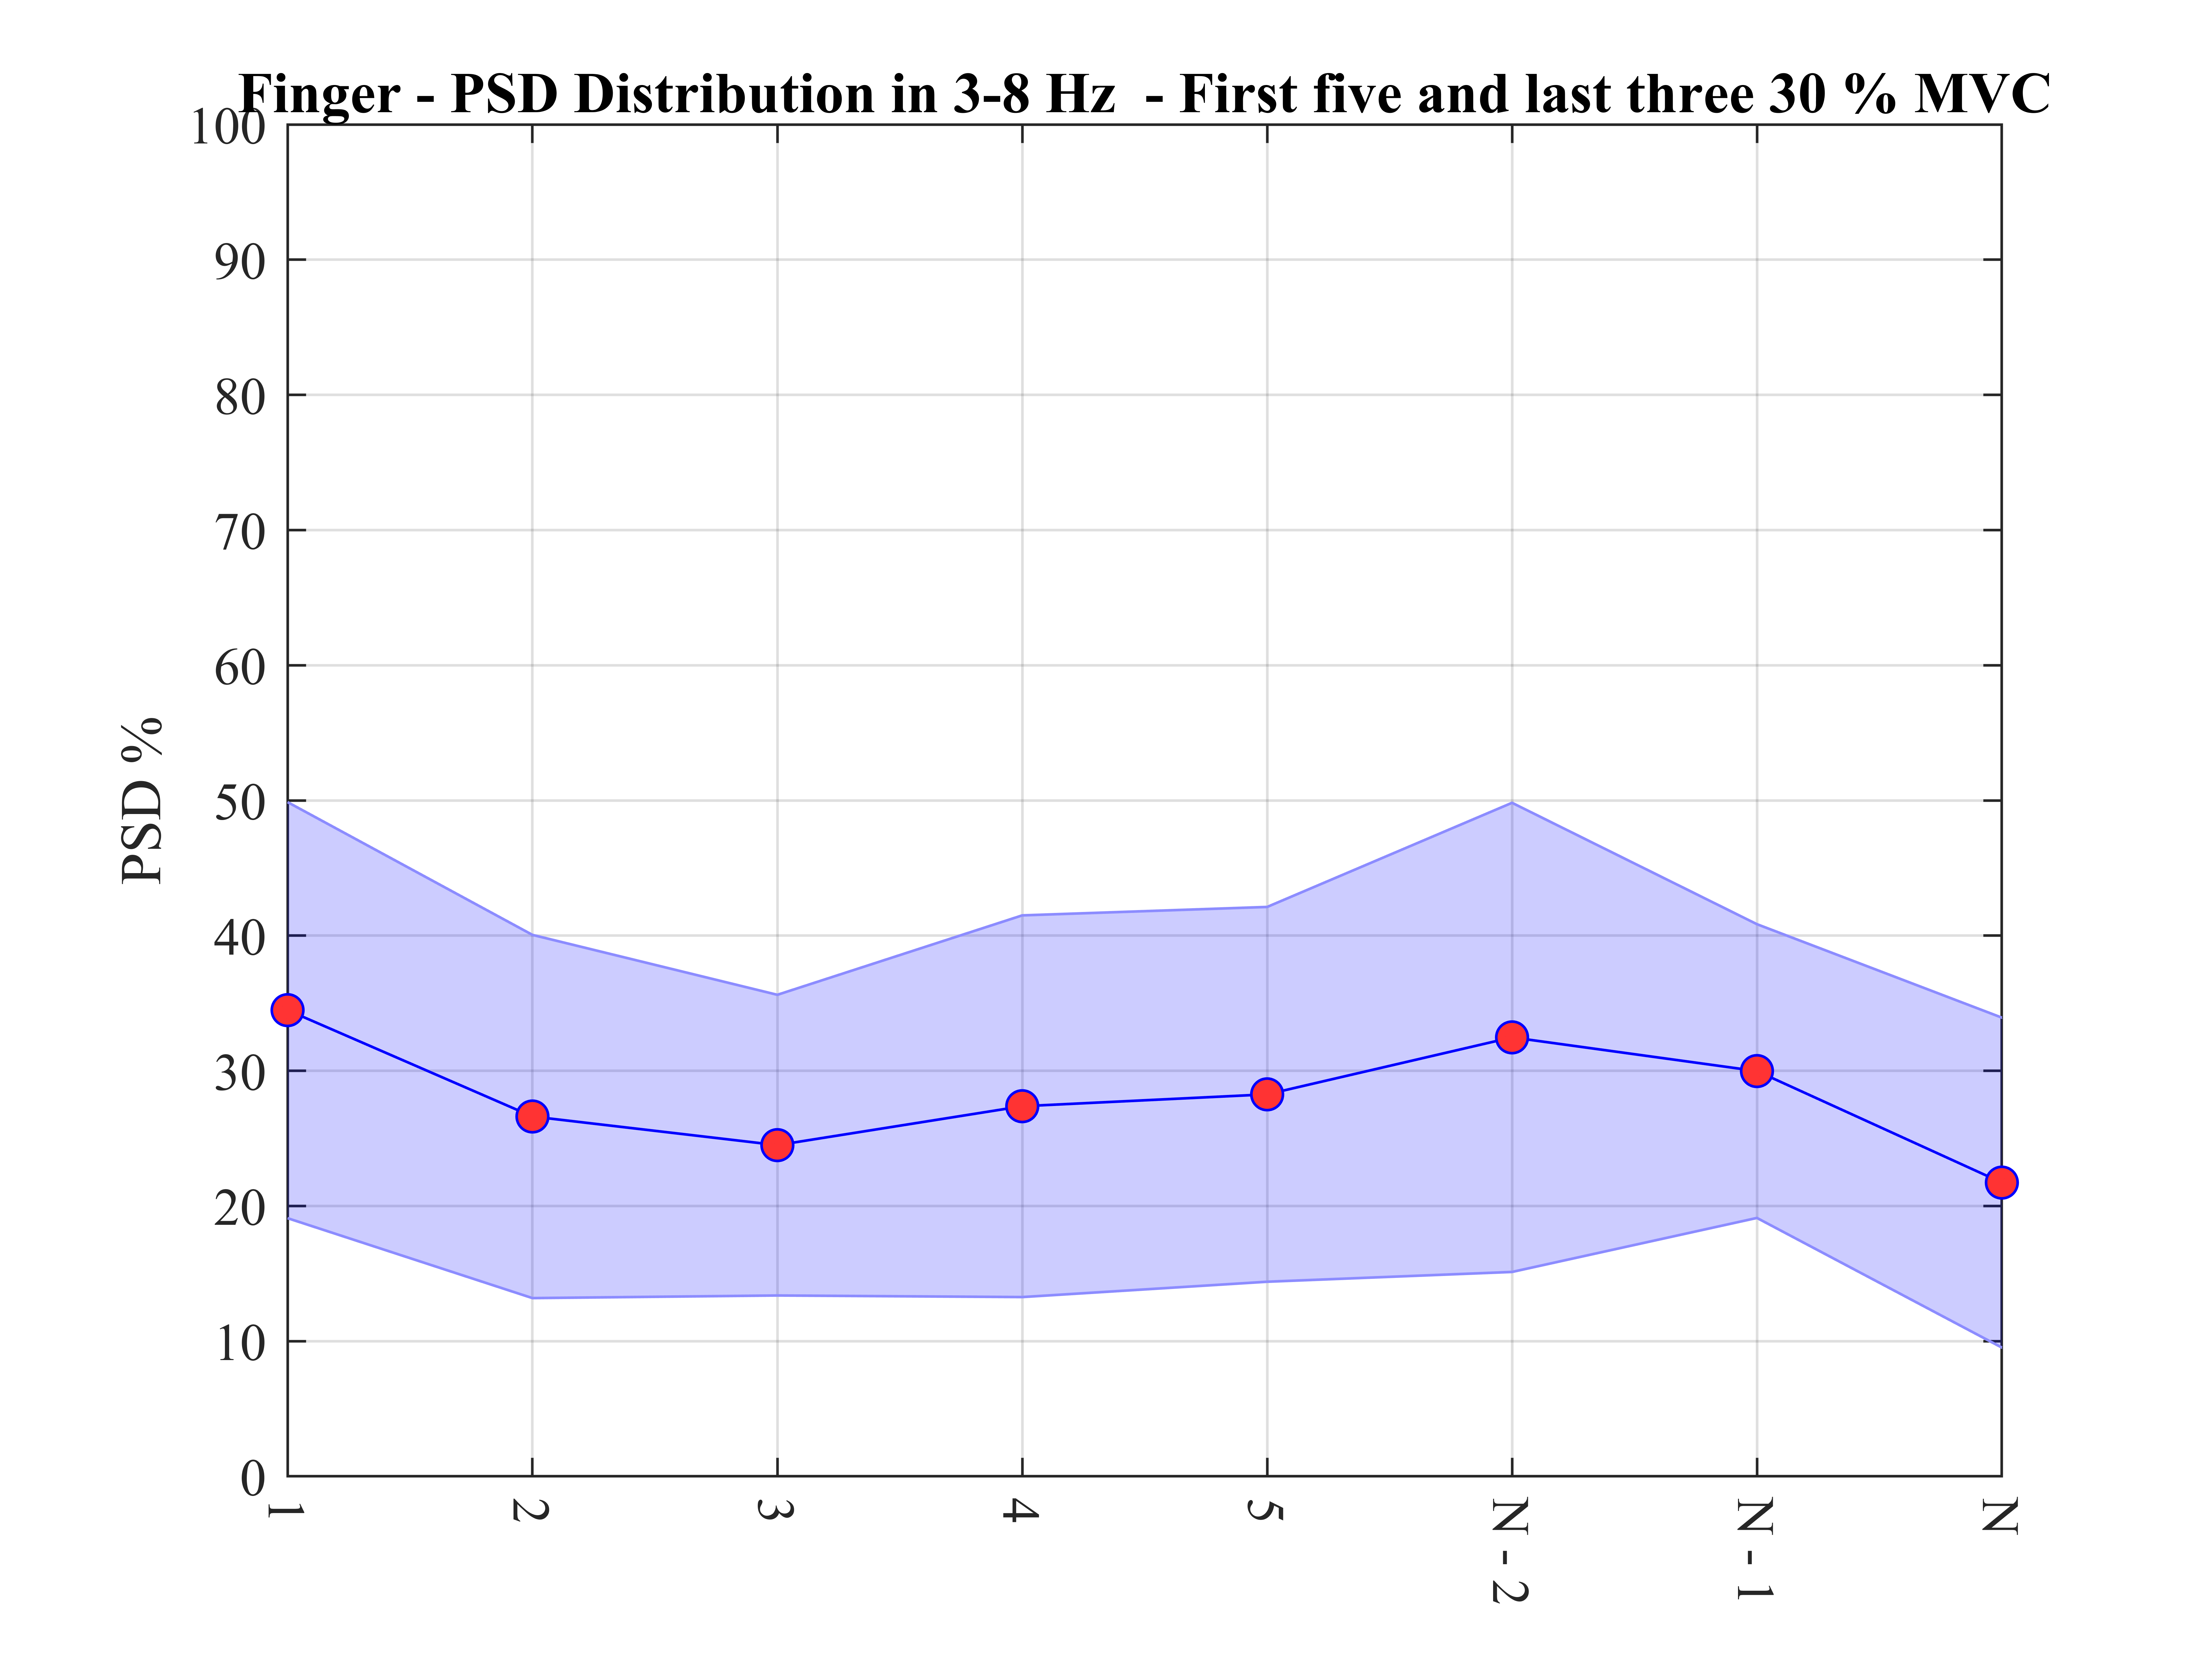
\includegraphics[width=0.31\textwidth]{Figures/finger_first_and_last_30_MVC-ept_shaded_3_8_fatigued.tex}}
	\label{fig:finger_first30MVC}
	\hfill
	\subfloat[Finger: 8 - 14 Hz]{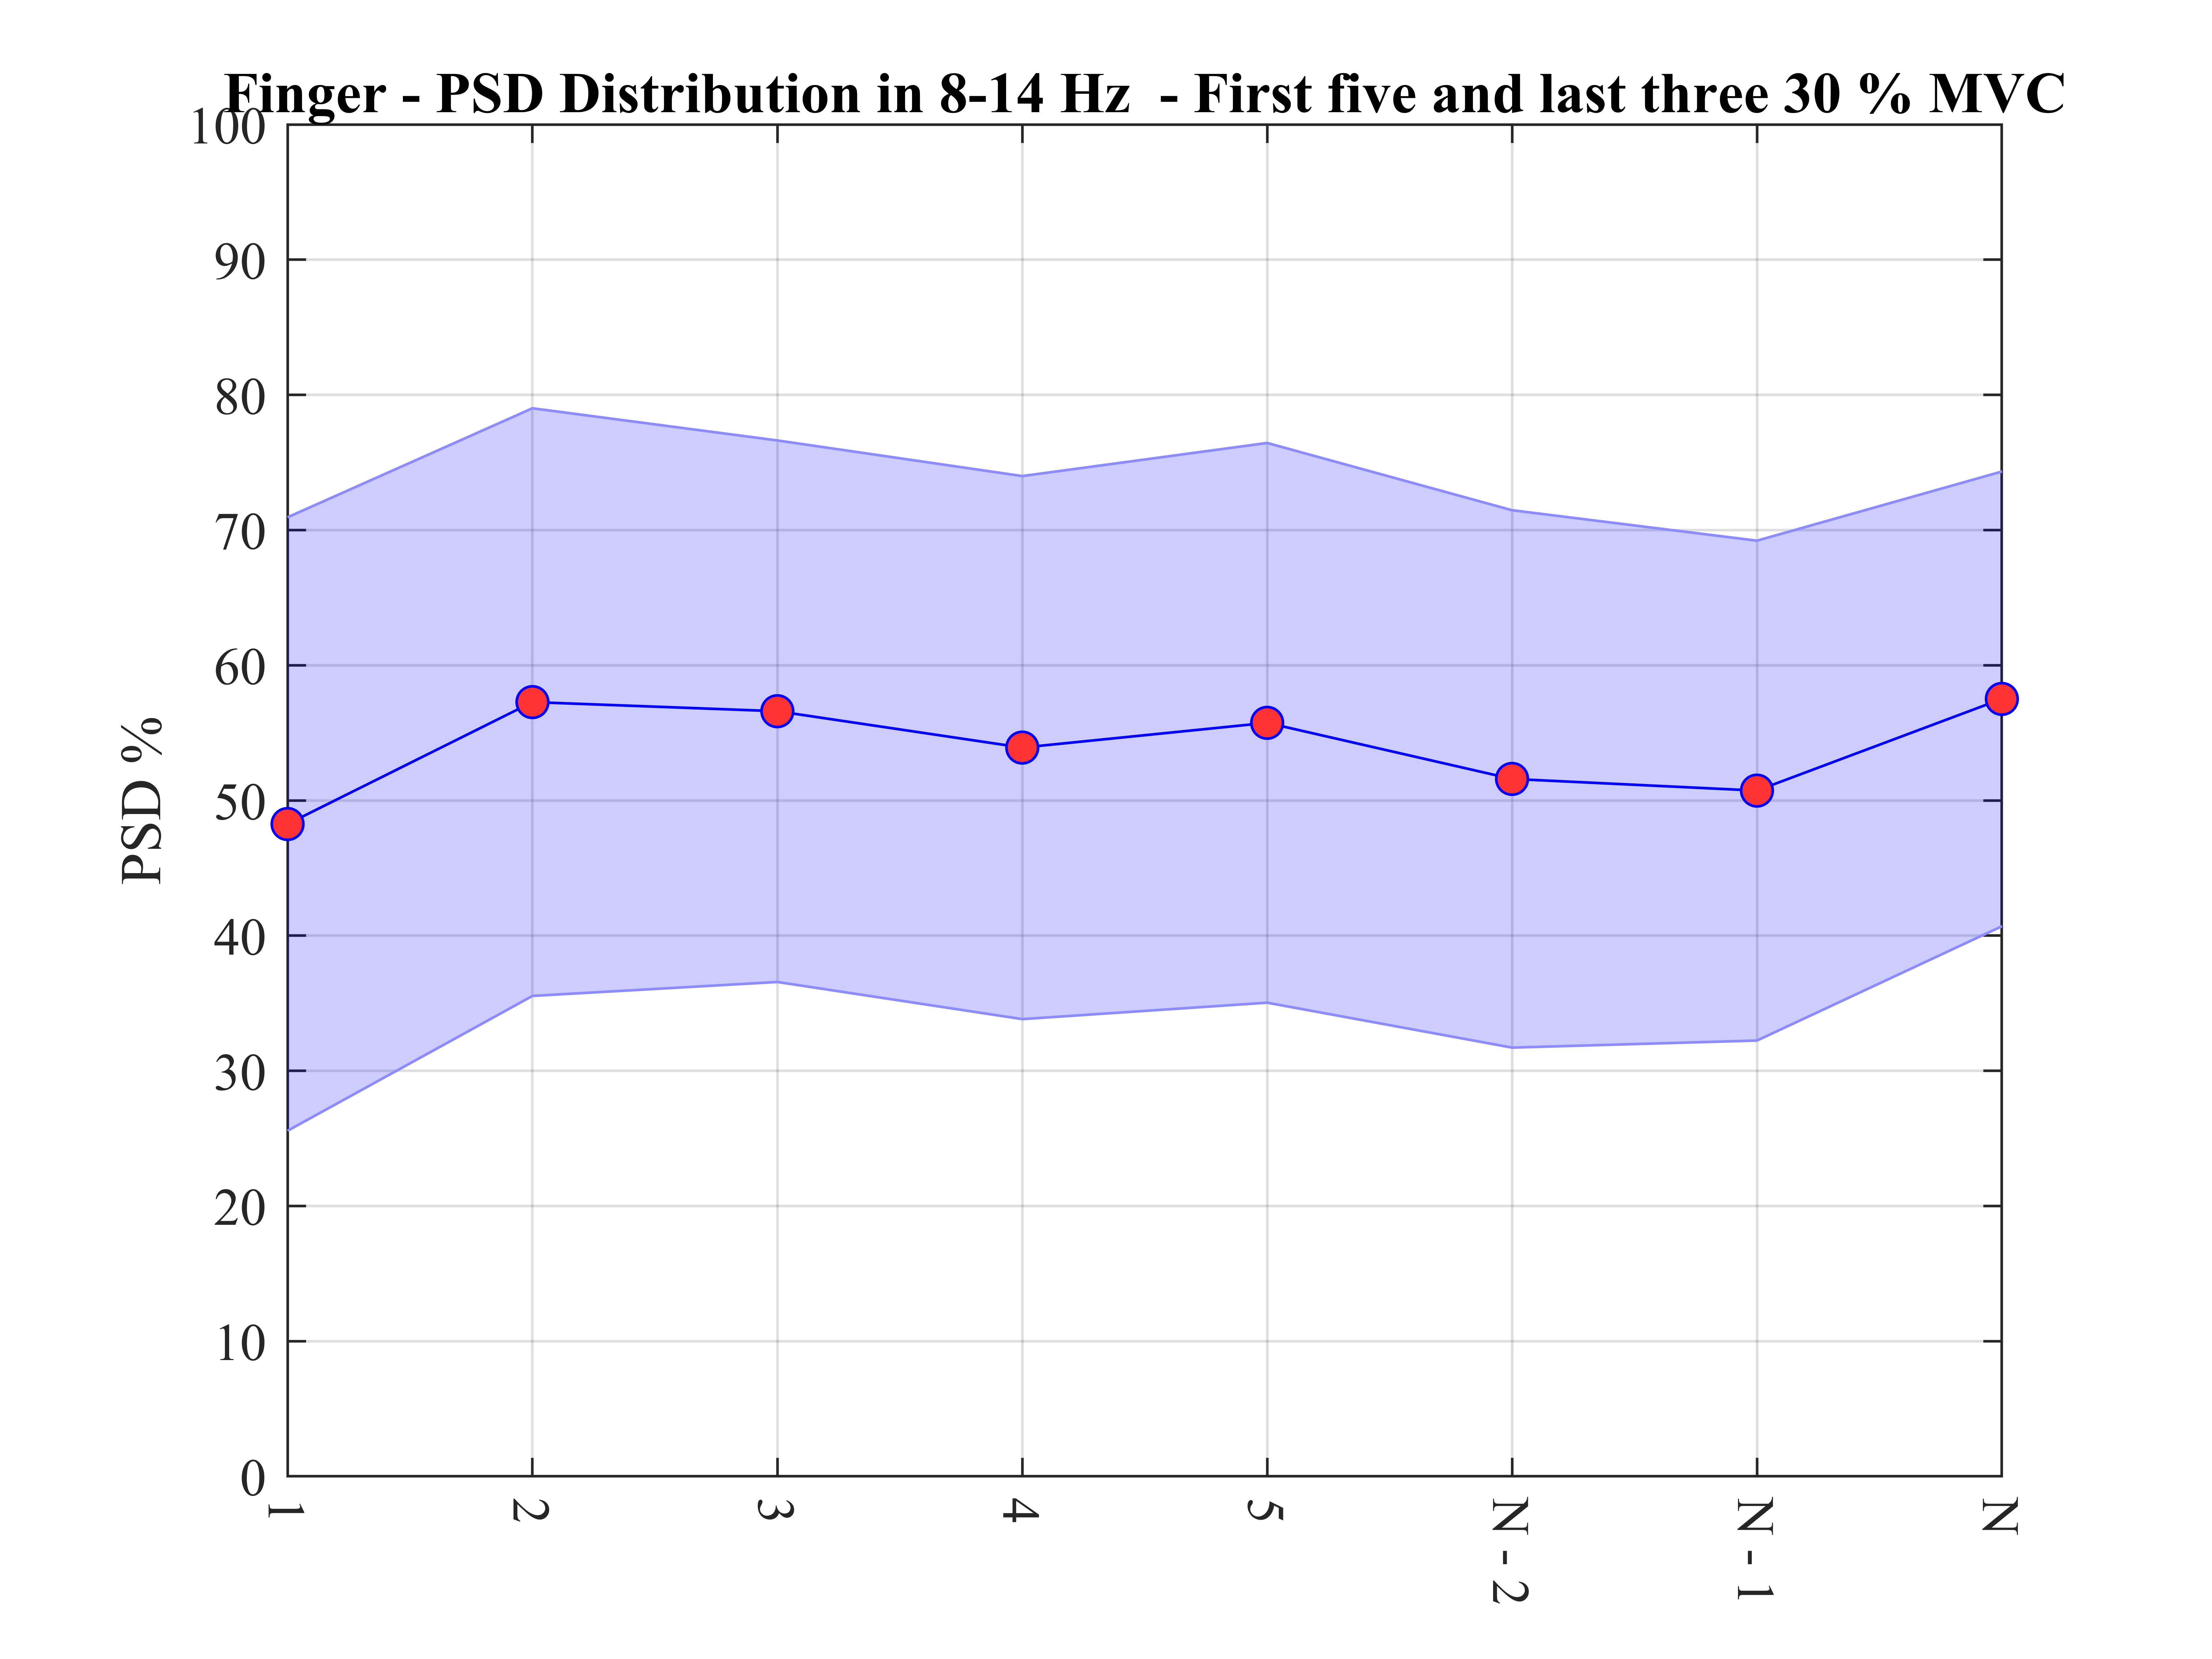
\includegraphics[width=0.31\textwidth]{Figures/finger_first_and_last_30_MVC-ept_shaded_8_14_fatigued.tex}}
	\label{fig:finger_first30MVC}
	\hfill
	\subfloat[Finger: 14 - 22 Hz]{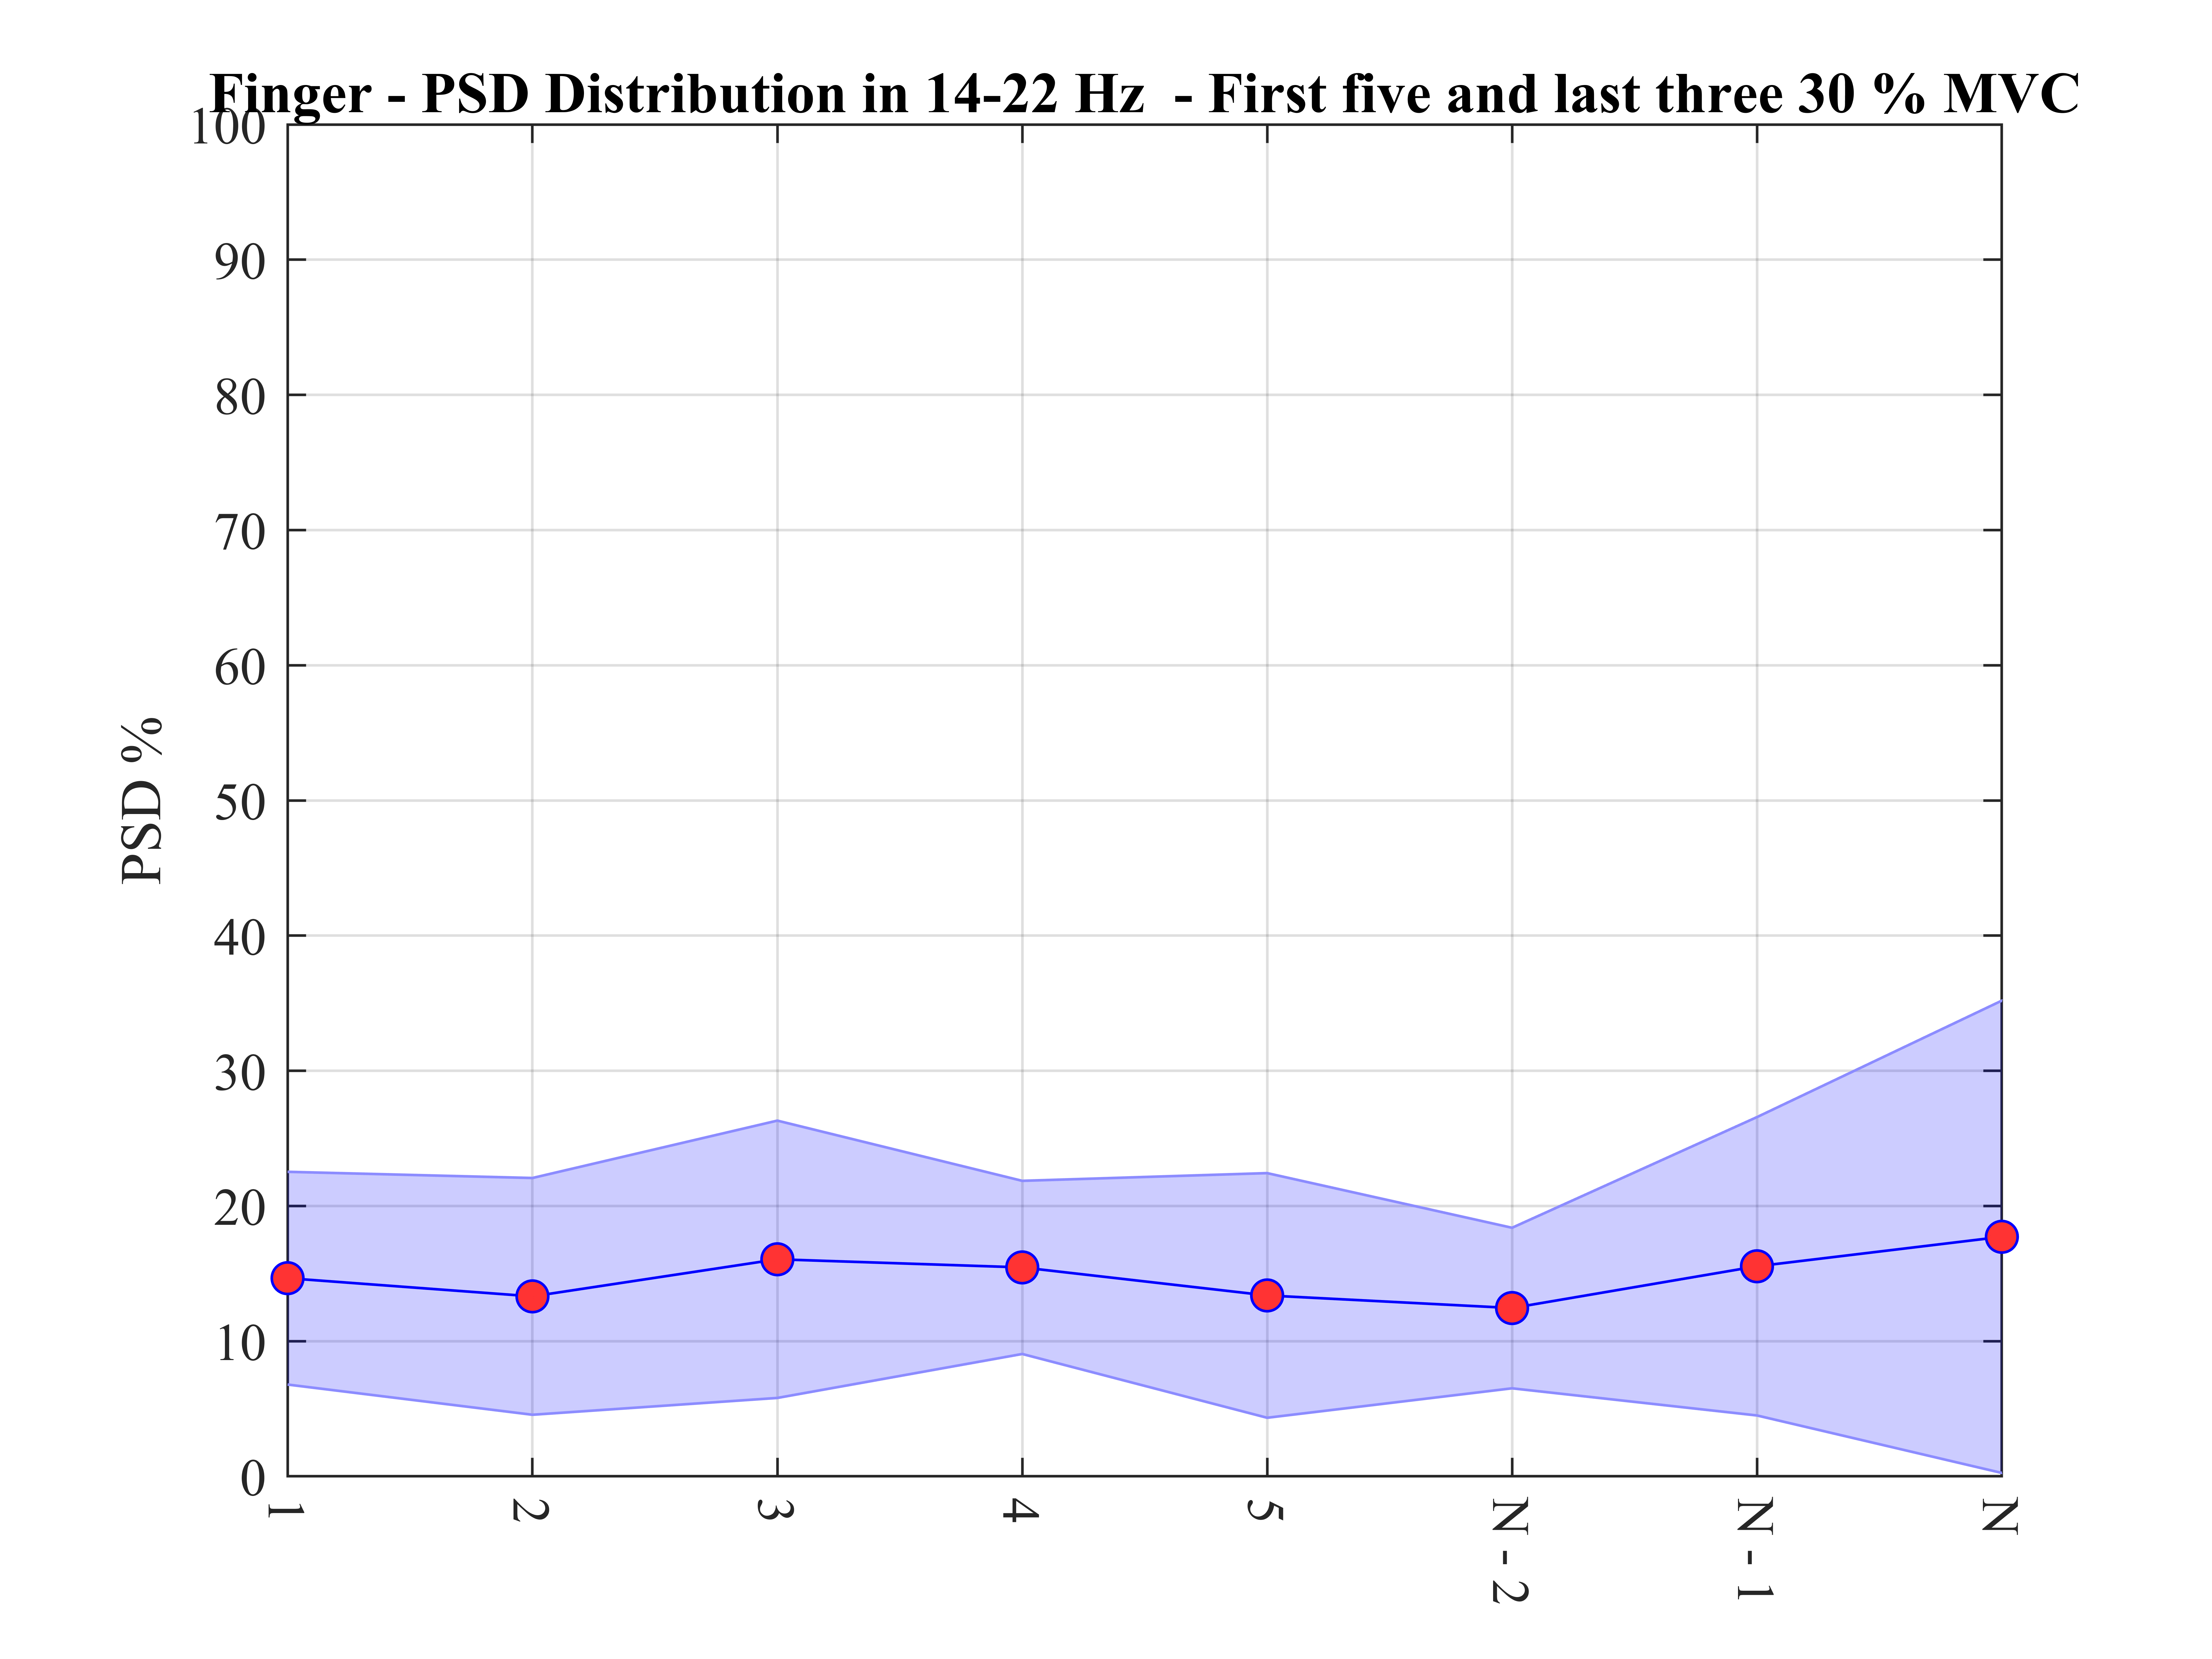
\includegraphics[width=0.31\textwidth]{Figures/finger_first_and_last_30_MVC-ept_shaded_14_22_fatigued.tex}}
	\label{fig:finger_first30MVC}	
	\caption{30\% MVC PSD distribution in different frequency ranges.}
	\label{fig:30_MVC}
\end{figure*}
% 
\subsection{Post Fatigue}

As each person has an individual level of fatigue the variance of the amplitude depends on personal physical condition. Exact after the exercises (0 min), the mean tremor's amplitude is almost the same as the pre-fatigue amplitude for finger and wrist in rest, posture and loaded posture conditions (Fig. \ref{fig:RMS}) but changes their mean PSD distribution.

As the participants continue with the exercises in posture and loaded posture condition, their fatigue increase. The rest time 1 min after the fatigue is 0 s. In posture condition case, the finger and wrist fatigue are most notable which is proved by the max variance of the tremor amplitude (Fig. \ref{fig:RMS}a,d) while the mean PSD distribution weakly decreases (Fig. \ref{fig:PSD}a).  The rests after the second and third post MVC are 120 and 240 s, respectively. This gives the opportunity of the participants to rest and the amplitude (Fig. \ref{fig:RMS}a,d) and mean PSD distribution and its variance (Fig. \ref{fig:PSD}) weakly decrease.
For PSD distribution in rest, posture and loaded posture conditions, the variance of the mean post-fatigue value is \SI{\pm 5}{\percent} compared with the pre-fatigue value (Fig. \ref{fig:PSD}). These small variances do not allow determining the fatigue influence on the PSD distribution.

For the finger tremor in rest and posture condition, the most notable changes of the post-fatigue mean PSD distribution and its variance are in the 3-8 Hz range.

%
\subsection{Maximum Voluntary Contraction}

In pre- and post-MVC case (Fig. \ref{fig:MVC}), the fatigue influence on the tremor amplitude is more notable on finger than on the wrist tremor as well as for the pre- and post-30\% MVC (Fig. \ref{fig:30_MVC}).
All participants do 3 cycles of pre-MVC with 60 s rest between them. Because of these rests the finger and wrist mean PSD distributions change weakly (Fig. \ref{fig:MVC}).
Observing the first five and last three 30\% MVC, the PSD distribution is more than 50\% for the finger and wrist in the frequency range 8-14 Hz (Fig. \ref{fig:30_MVC}b). For the rest two ranges, the values are between 20 and 30\%.

The post-MVC cycles include consecutive execution of rest, posture and loaded posture condition. The rest time increase from 0 to 4 min. From Fig. \ref{fig:MVC}, can be noticed that in the range 8-14 Hz mean PSD distribution increase between post-1min and post-5min as the fatigue increase. The decreasing in the interval post-5min to post-10min shows that the number of tremors with frequency 8-14 Hz also decrease at the expense of tremors in the 3-8 Hz range, which are typical for the rest condition. These changes are not so notable for wrist tremor. For the MVC and 30\% MVC conditions (Fig. \ref{fig:30_MVC}), the tremor can be detected better on the wrist because the mean PSD distribution values in the 8-14 Hz range are with almost 30\% bigger than values in the 3-8 and 14-22 Hz, i.e. the main part of the tremors is with frequency typical for PT.

We did not find any dependence between the rest and action tremor frequencies or amplitudes based on the gender, blood pressure, pulse, and age of the participants.
%
% \FloatBarrier
\section{Conclusion}
%
This paper presents the spectral analysis of hand tremors recorded from the finger and the wrist. For the study, a low-cost and wearable hand tremor sensing device was designed using a 3 axis accelerometer. It was observed that the physiologic tremor in the frequency range of 8-14 Hz was most noticeable during the fatigue inducing tasks involving maximum voluntary contraction. Moreover, the power spectral density showed a uniform distribution during the tasks that did not involve any physical exertion. The outcomes of this study provide motivation that physiological conditions, such as hypoglycemia that cause enhanced physiologic tremors, can be detected using the developed sensors.
%%%%%%%%%%%%
%%%%%%%%%%%%%%%%
%%%%%%%%%%%%%%%%
%%%%%%%%%%%%%%%%
%%%%%%%%%%%%%%%%
%%%%%%%%%%%%%%%%
%%%%%%%%%%%%%%%%
%%%%%%%%%%%%%%%%
\section{Acknowledgment}
%
This publication was made possible by NPRP grant number NPRP 10-1231-160071 from the Qatar National Research Fund (a member of Qatar Foundation). The statements made herein are solely the responsibility of the authors.
%
\bibliographystyle{IEEEtran}
% \atColsEnd{\vfil}
% argument is your BibTeX string definitions and bibliography database(s)
\bibliography{references}
\end{document}
